\documentclass[pdflatex,en,11pt]{aghdpl}
\usepackage[english]{babel}
\usepackage{polski}
\usepackage[utf8]{inputenc}

\usepackage[backend=bibtex,
style=numeric,
%bibencoding=ascii,
%style=reading
]{biblatex}

\addbibresource{bibliografia.bib}

\DeclareNameAlias{sortname}{last-first}
\DeclareNameAlias{default}{last-first}

% dodatkowe pakiety
\usepackage{enumerate}
\usepackage{listings}
\usepackage{float}
\usepackage{siunitx}
\usepackage{hyperref}
\usepackage[acronym,nomain,toc]{glossaries}

% \lstloadlanguages{TeX}

\lstset{
  literate={ą}{{\k{a}}}1
           {ć}{{\'c}}1
           {ę}{{\k{e}}}1
           {ó}{{\'o}}1
           {ń}{{\'n}}1
           {ł}{{\l{}}}1
           {ś}{{\'s}}1
           {ź}{{\'z}}1
           {ż}{{\.z}}1
           {Ą}{{\k{A}}}1
           {Ć}{{\'C}}1
           {Ę}{{\k{E}}}1
           {Ó}{{\'O}}1
           {Ń}{{\'N}}1
           {Ł}{{\L{}}}1
           {Ś}{{\'S}}1
           {Ź}{{\'Z}}1
           {Ż}{{\.Z}}1
}

\newcommand{\rad}{\radian}
\newcommand{\iic}{$I^2C$ }
\newcommand{\uA}{\micro\ampere}
\newcommand{\mA}{\milli\ampere}
\newcommand{\uV}{\micro\volt}
\newcommand{\mV}{\milli\volt}

\usepackage{array}
\newcolumntype{L}[1]{>{\raggedright\let\newline\\\arraybackslash\hspace{0pt}}m{#1}}
\newcolumntype{C}[1]{>{\centering\let\newline\\\arraybackslash\hspace{0pt}}m{#1}}
\newcolumntype{R}[1]{>{\raggedleft\let\newline\\\arraybackslash\hspace{0pt}}m{#1}}

\makeatletter
\let\ps@plain\ps@fancy
\makeatother

%---------------------------------------------------------------------------

\author{Grzegorz Gajoch}
\shortauthor{G. Gajoch}

\course{Electronics and Telecommunications}

\titlePL{Budowa sensora pochłoniętej dawki promieniowania jonizującego (TID) dla nano-satelitów typu CubeSat}
\titleEN{Total Ionizing Dose (TID) sensor for CubeSat~nano-satellites}

\shorttitlePL{Budowa sensora pochłoniętej dawki promieniowania jonizującego (TID) dla nano-satelitów typu CubeSat} % skrócona wersja tytułu jeśli jest bardzo długi
\shorttitleEN{Total Ionizing Dose (TID) sensor for CubeSat~nano-satellites}

\thesistypePL{Praca dyplomowa inżynierska}
\thesistypeEN{Engineering Thesis}

\supervisorPL{dr inż. Cezary Worek}
\supervisorEN{Cezary Worek Ph.D}

\date{2016}

\departmentPL{Katedra Elektroniki}
\departmentEN{Department of Electronics}

\facultyPL{Wydział Informatyki, Elektroniki i Telekomunikacji}
\facultyEN{Faculty of Computer Science, Electronics and Telecommunications}

\acknowledgements{}

\setlength{\cftsecnumwidth}{10mm}


%---------------------------------------------------------------------------

\begin{document}

\titlepages

\tableofcontents
\clearpage

\chapter{Terms, definitions and abbreviated terms}

    \section{Abbreviated terms}

    \section{Conventions}

\chapter{Introduction}
    Ionizing radiation is one of the major concerns during space mission development, both manned and unmanned. Just as the human body is affected by radiation, so are electronic components, which will fail under certain conditions.

    A special design methodology, radiation hardening, must be implemented for all satellite components, which dramatically increases mission costs. Some assumptions are made during satellite planning, such as radiation tolerance, above which the mission can fail. Absorbed dose can be predicted by simulations, but unusual events like solar flares can alter predictions to unacceptable levels. For monitoring the absorbed dose, most satellites have on-board Total Ionizing Dose (TID) sensors, allowing to deorbit or move satellite to graveyard orbit before it fails.

    Usually, these sensors are very expensive and it is hard to cut the cost due to custom ASIC design. They are also large and require a lot of power to operate. However, recent publications suggest that Commercial Off-The-Shelf (COTS) transistors can be used to assemble an absorbed dose sensor.

    To date, very few small student-satellites (e.g. CubeSats) have TID sensors on-board. This is mainly due to their cost, but also to limited time, space and power resources. At present, this sensor is not critical in Low Earth Orbit (LEO), when, following failure, a satellite will deorbit by means of atmospheric drag. In the near future, as a consequence of expanding CubeSat market beyond LEO, the possibility of satellite collisions is expected to grow significantly. This will force CubeSats to start implementing more radiation-hardening techniques, which, on pico- and nano-satellites, mainly consists of COTS components screening, radiation tests and real-time operation monitoring. This opens the need for CubeSat TID sensors, which are currently not available on the market.

    In this thesis, the design of an absorbed dose sensor is presented. The thesis aims at presenting design requirements and solutions, along with simulations and preliminary tests. The presented sensor is planned to be flown on-board PW-Sat2 student satellite, in Q4 2017.

\newpage
    Brief description of thesis chapters:
    \begin{itemize}
        \item Abbreviations, conventions - present abbreviations and conventions used within this thesis,
        \item Introduction - this chapter, description of the thesis aims,
        \item Principles - introduces reader to radiation related problems and explains the theory of operation,
        \item Requirements - presents design requirements for this particular sensor, because it is designed specifically for PW-Sat2 satellite,
        \item Sensor design - presents high-level sensor design phase, explaining its operation on block and system level,
        \item Engineering model - describes the sensor model developed during this thesis, its design and simulations,
        \item Tests - presents results of conducted sensor tests,
        \item Future work - briefly describes the required next steps until flight solution is ready,
        \item Summary - summarizes thesis, work and outcome.
    \end{itemize}

\chapter{Principles}

\section{Radiation effects on electronic devices}
    There are two basic effects of radiation on silicon components:
    \begin{itemize}
        \item ionizing effect
        \item displacement damage
    \end{itemize}

    Those two effect are responsible for changing parameters of semiconductor devices, which after some time can lead to failure of the device. Main source of this radiation are Gamma (ionization) and Neutron particles (displacement).

    In space electronics during analysis and design two major problems are considered - Single Event Effects (SEE) and Total Ionizing Dose (TID). Every silicon and silica device is susceptible to both of those - and both have to be considered during product design, development and testing.

    \subsection{Single Events Effects}
        Single Event Effects are connected with generation of electron-hole pair in semiconductor, when material is exposed to ionizing radiation. Amount of pairs generated is proportional to energy deposited. For semiconductor device parameter $LET_{th}$ (Linear Energy Transfer Threshold) is defined, being a measure of how susceptible the device is. For particles with Linear Energy Transfer (LET - normalized particle energy per mass of the absorbing material), below this threshold no effect will be observed.

        Single Event Effects are divided into two groups - non-destructive (fully recoverable, possibly after power cycle) and destructive (permanent damage) effects. Shortly those are described below, defined as in \cite{ECSS_Q_ST_60_15C}.

        \bigskip\textbf{Non-destructive effects}
        \begin{itemize}
            \item \textbf{Single Event Upset} - especially memory-based devices (like microprocessors, memories, Field Programmable Gate Array - FPGA) are vulnerable. This phenomenon will possibly alter the state of cell in memory - causing memory corruption. This can lead to complete failure of device if this is not corrected.

            \item \textbf{Single Event Functional Interrupt} - subset of SEU - this effect cause the system to latch in non-recoverable state (e.g. by switching to wrong state in state machine). Only option is to reset circuit to back to known state.

            \item \textbf{Single Event Transient} - are formed as a voltage/current spurious pulses generated by charge induced by striking particle. This can cause different problems - from disturbing analog electronics up to causing switch of digital circuit. This effect strongly depends on size of feature in silica.
        \end{itemize}

        \bigskip\textbf{Destructive effects}
        \begin{itemize}
            \item \textbf{Single Event Latch-up} - particle striking can cause turning on parasitic thyristor in CMOS structure. This will lead to effectively shorting voltage supply to ground, causing overheat and damage to the device.

            \item \textbf{Single Event Gate Rupture} - high energy particle comes through thin gate (especially in MOS transistors) can cause generation of electron-holes pairs in gate and substrate - causing high electric field across gate. When this effect is strong enough it can cause permanent damage to transistor.

            \item \textbf{Single Event Burnout} - ion that traverses the transistor structure (through the source) can induce a current flow that turns on the parasitic npn transistor. This leads to effective short circuit and damage to the device.
        \end{itemize}

        \bigskip\textbf{Mitigation techniques}

        Below recommended mitigation techniques for SEE were listed:
        \begin{itemize}
            \item SEU - redundancy, memory scrubbing,
            \item SEFI - watchdog, proper reset sequence,
            \item SET - use lower-integration scale devices, implement protection resistors etc.
            \item SEL - implement overcurrent circuits (like Latch-up Current Limiters),
            \item SEGR, SEB - use higher $LET_{th}$ devices
        \end{itemize}

    \subsection{Total Ionizing Dose}
        TID is defined as total energy absorbed during exposure. This can be caused by any kind of radiation, behaving differently in every semiconductor device. In general, TID successively degrades electronic device parameters in time, causing them to stop functioning when critical irradiation was reached. Effect in p-MOSFET transistor is described in section \ref{Radiation_effects_on_MOS_transistors}.

        Every qualified device for spacecraft system will have tested value of TID value, for example by MIL-STD-883G, Test Method 1019.7 \cite{MIL_STD_883}. For example, ADC128S102QML-SP have a guaranteed value of 100 kRad.

\section{Need for TID radiation dosimetry}
    During spacecraft mission accumulated radiation level should be monitored to not excess guaranteed values for components. For example, near end of its lifetime, spacecraft can be commanded to deorbit into atmosphere or move to parking orbit - before fail can occur, causing losing control of spacecraft.
    Absorbed dose simulation and estimation is possible, but results are averaged by long period of time. Constantly flying by South Atlantic Anomaly or Van Allen belts can cause radiation estimation to be inaccurate, so near all spacecrafts implement sensor which constantly monitor radiation level absorbed by its electronics.

\section{On-line TID radiation dosimetry}

\section{RadFET Theory}

    \subsection{Radiation effects on MOS transistors}
    \label{Radiation_effects_on_MOS_transistors}

    \subsection{Threshold voltage measurement}

    \subsection{Temperature dependencies}

\chapter{Design requirements}

In this chapter the requirement for the TID sensor will be presented.

Sensor is designed to be flown on-board of PW-Sat2 satellite. Therefore it should be designed for its particular requirements. In addition, it should be designed having in mind active space standard and launcher requirements.


\section{PW-Sat2}
    Presented sensor is scheduled to be launched on PW-Sat2 satellite \cite{PW-Sat2URL}. Therefore it should be designed especially for this particular type of mission. In this section PW-Sat2 mission will be presented. 

    On fig. \ref{PW-Sat_render_01} exploded render of PW-sat2 is presented.

    \begin{figure}[h]
        \centering
        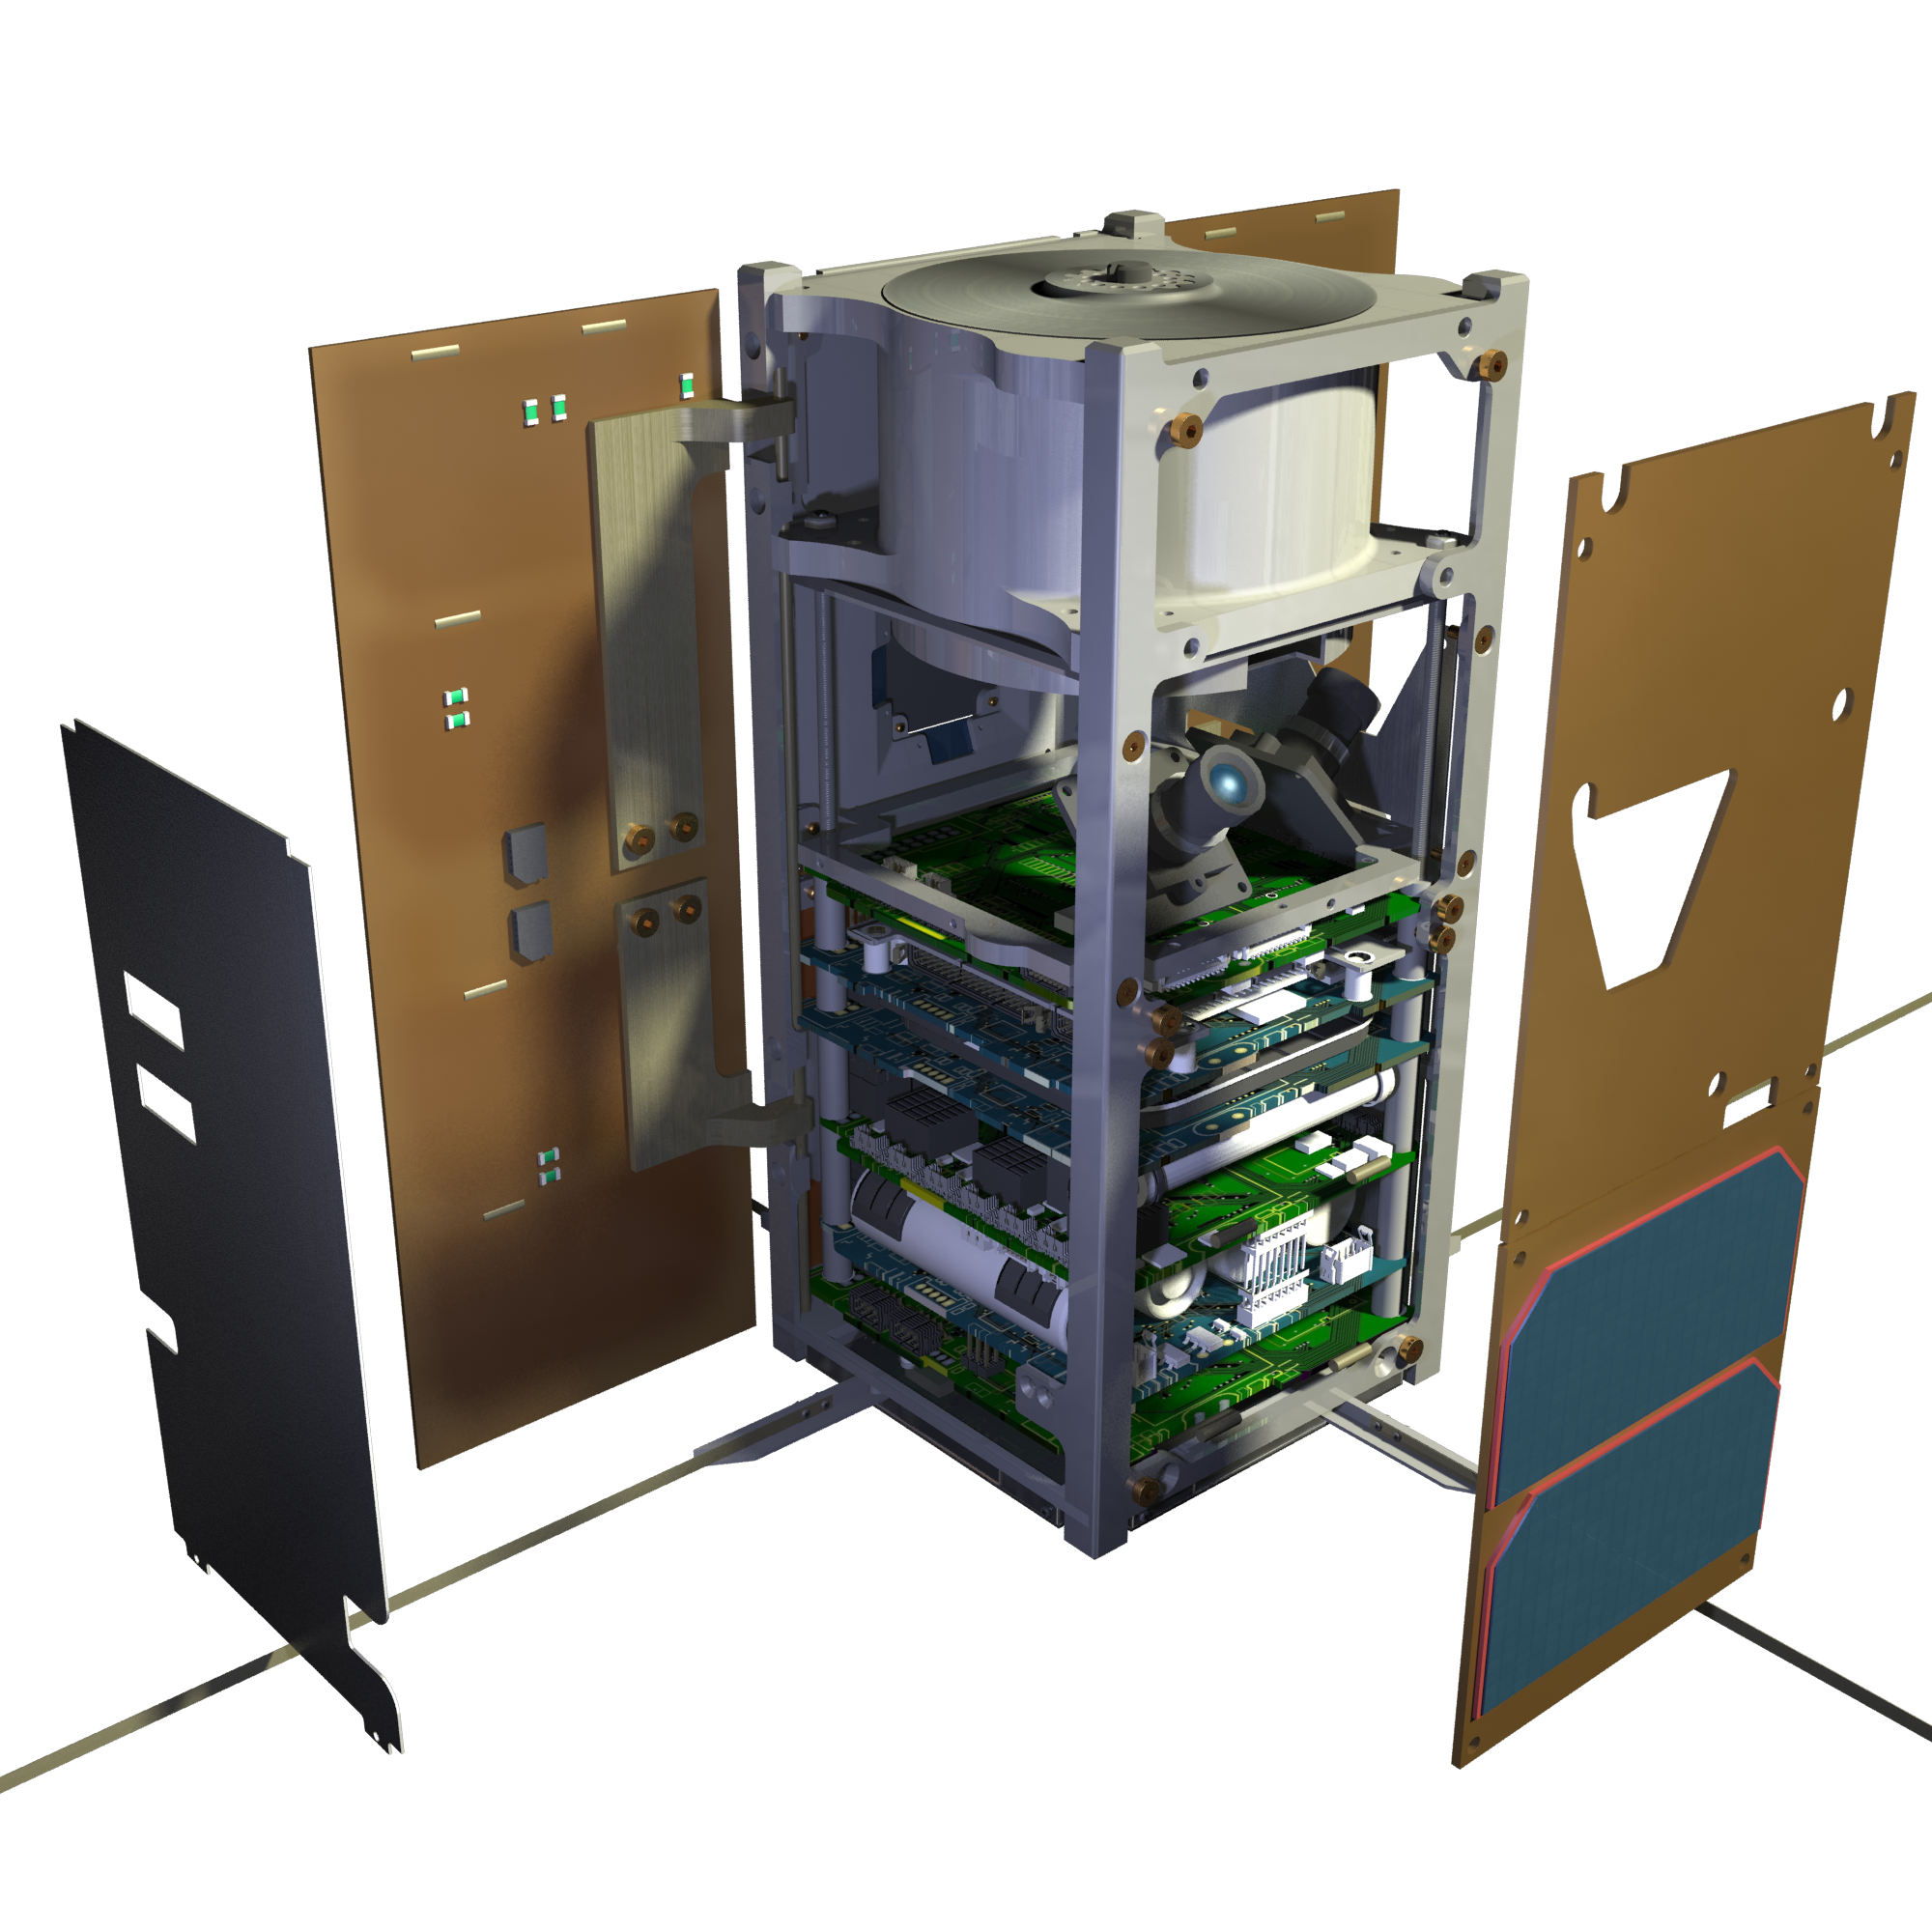
\includegraphics[width=0.5\paperwidth]{img/PW-Sat2_render_01.png}
        \caption{PW-Sat2 render (by M. Świetlik)}
        \label{PW-Sat_render_01}
    \end{figure}

    PW-Sat2 is scheduled to be launched on Falon9 rocket from SpaceX company in Q4 2017.

    \begin{figure}[H]
        \centering
           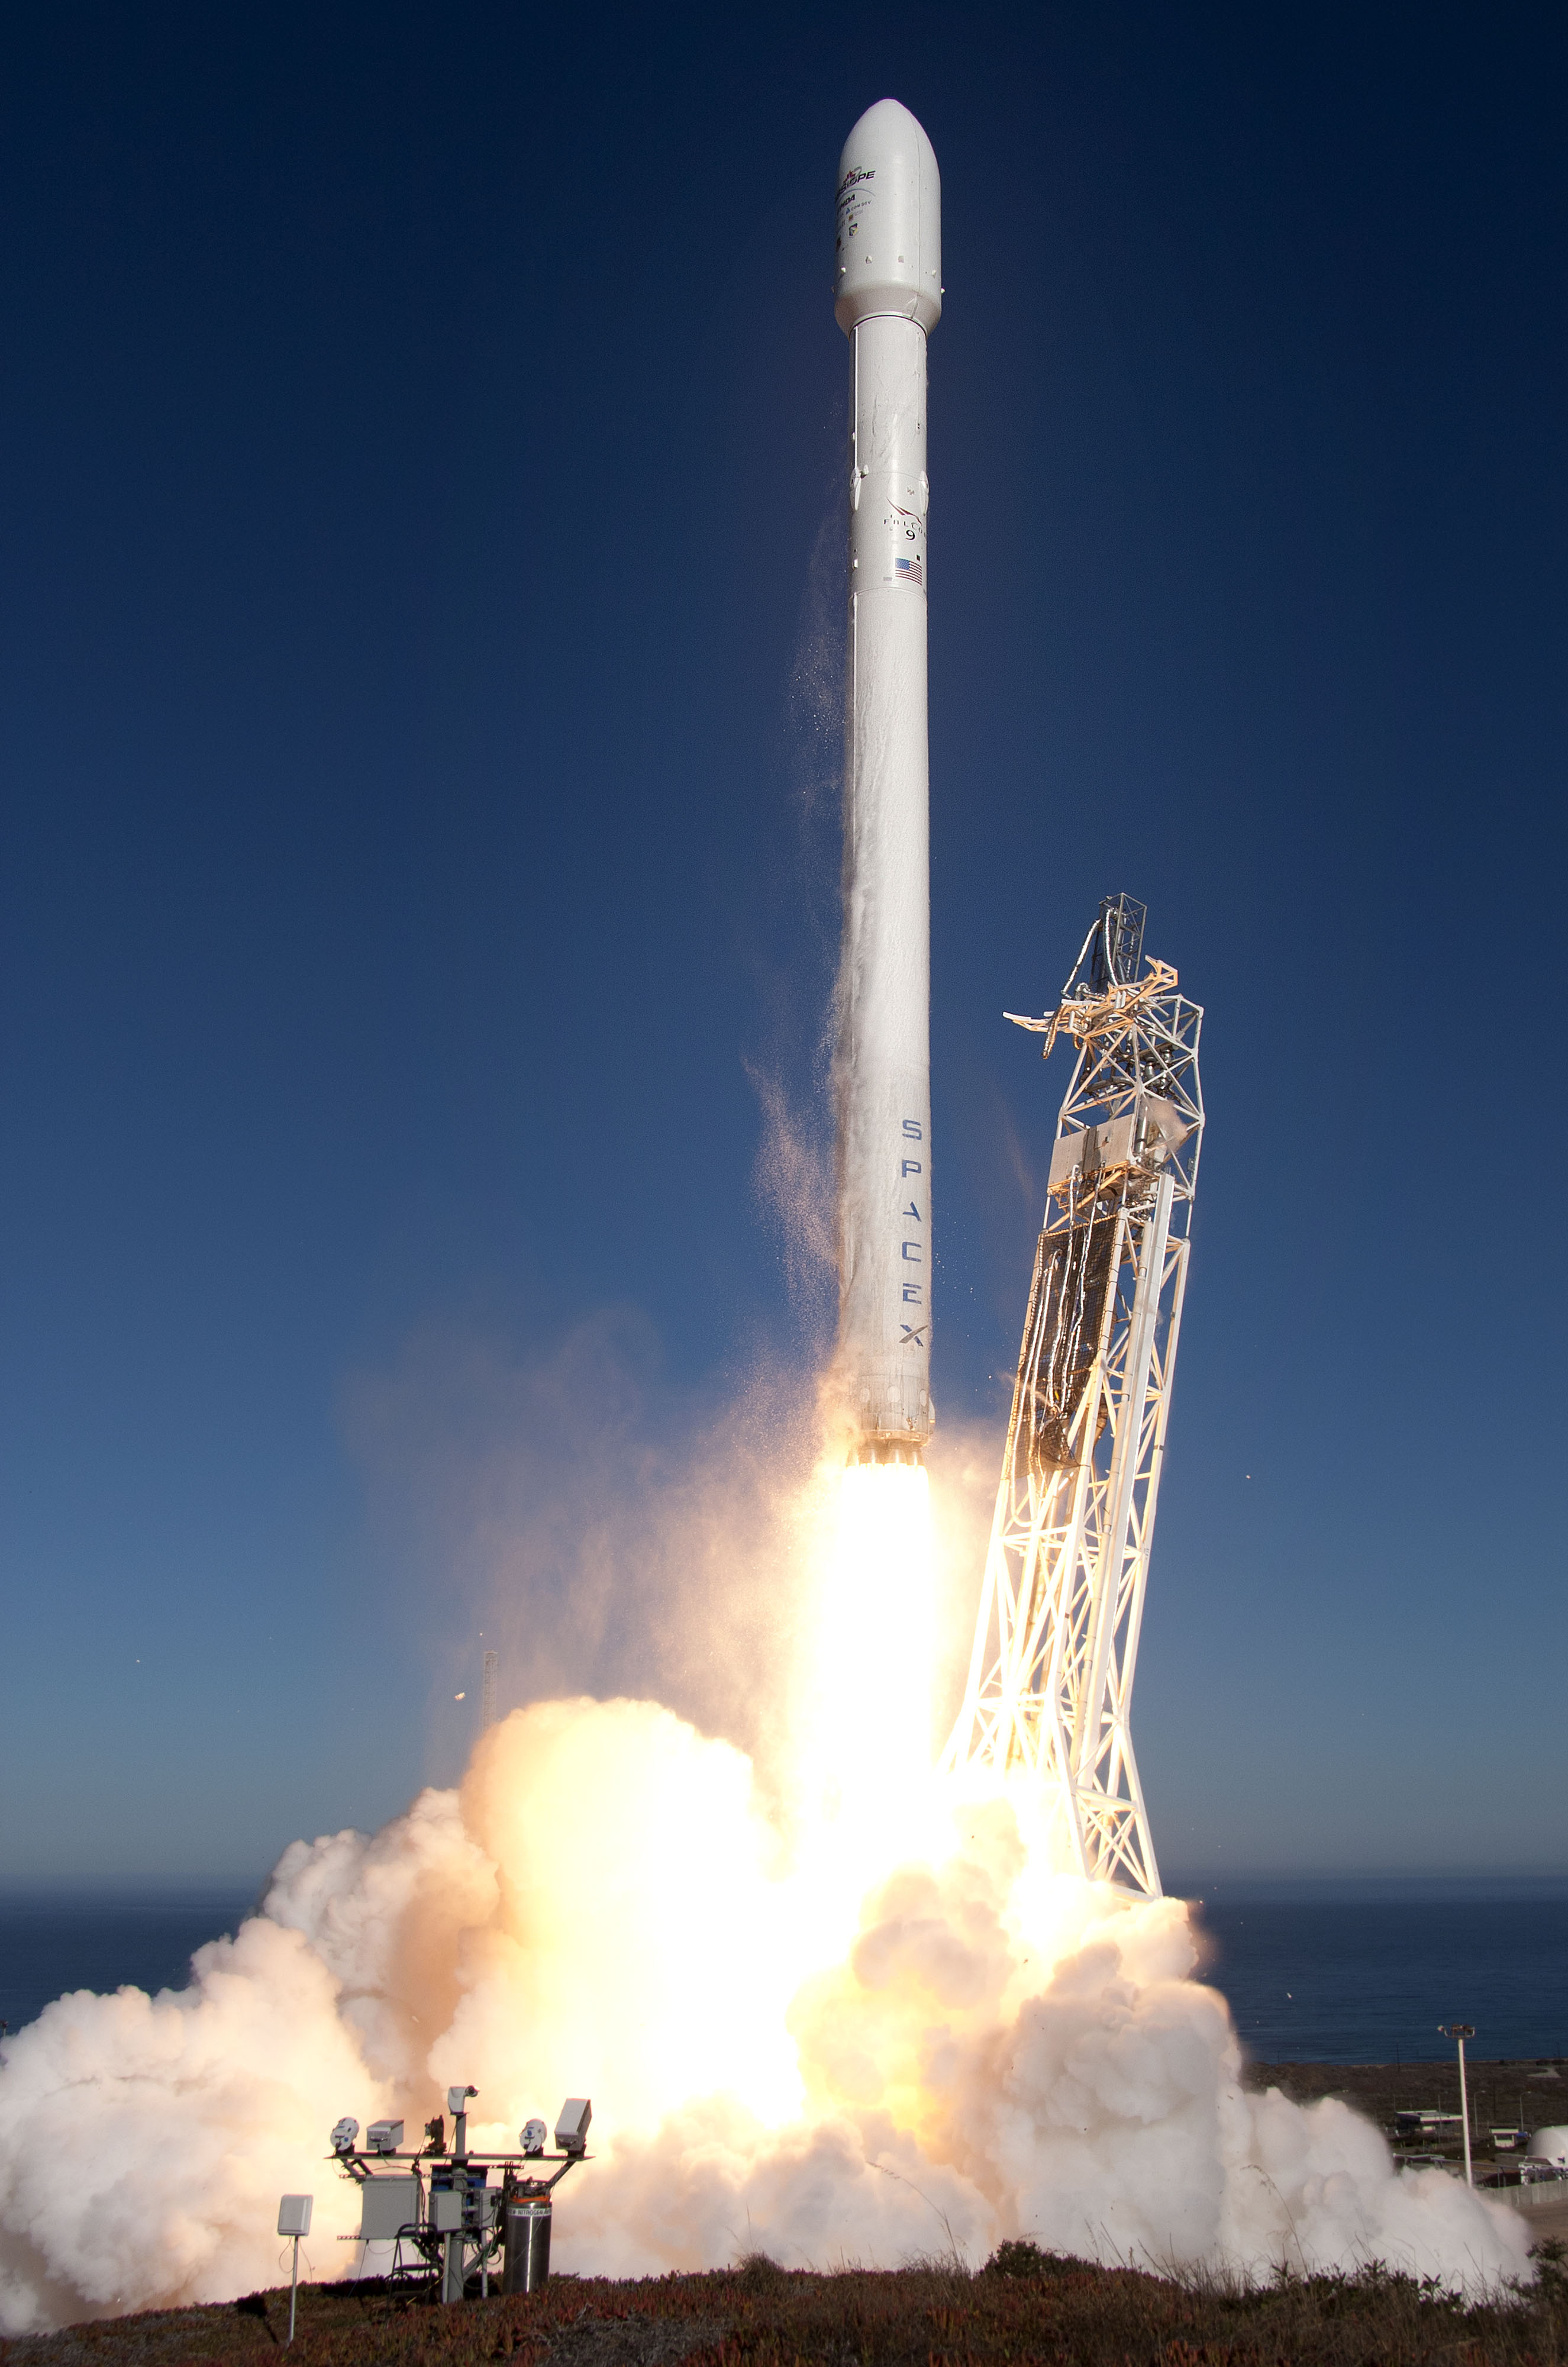
\includegraphics[width=0.3\paperwidth]{img/Falcon9.jpg}
        \caption{Falcon9 rocket. Source: \url{www.spacex.com}}
        \label{PW-Sat_render_01}
    \end{figure}


\subsection{Primary mission}
    Primary mission of PW-Sat2 is to test deorbit sail. Its purpose is to increase atmospheric drag and shorten satellite life. This method of deorbitation could be easy way to reduce space debris on LEO. Render of PW-Sat2 with opened sail is on \ref{PW-Sat_render_sail}.

    \begin{figure}[H]
        \centering
        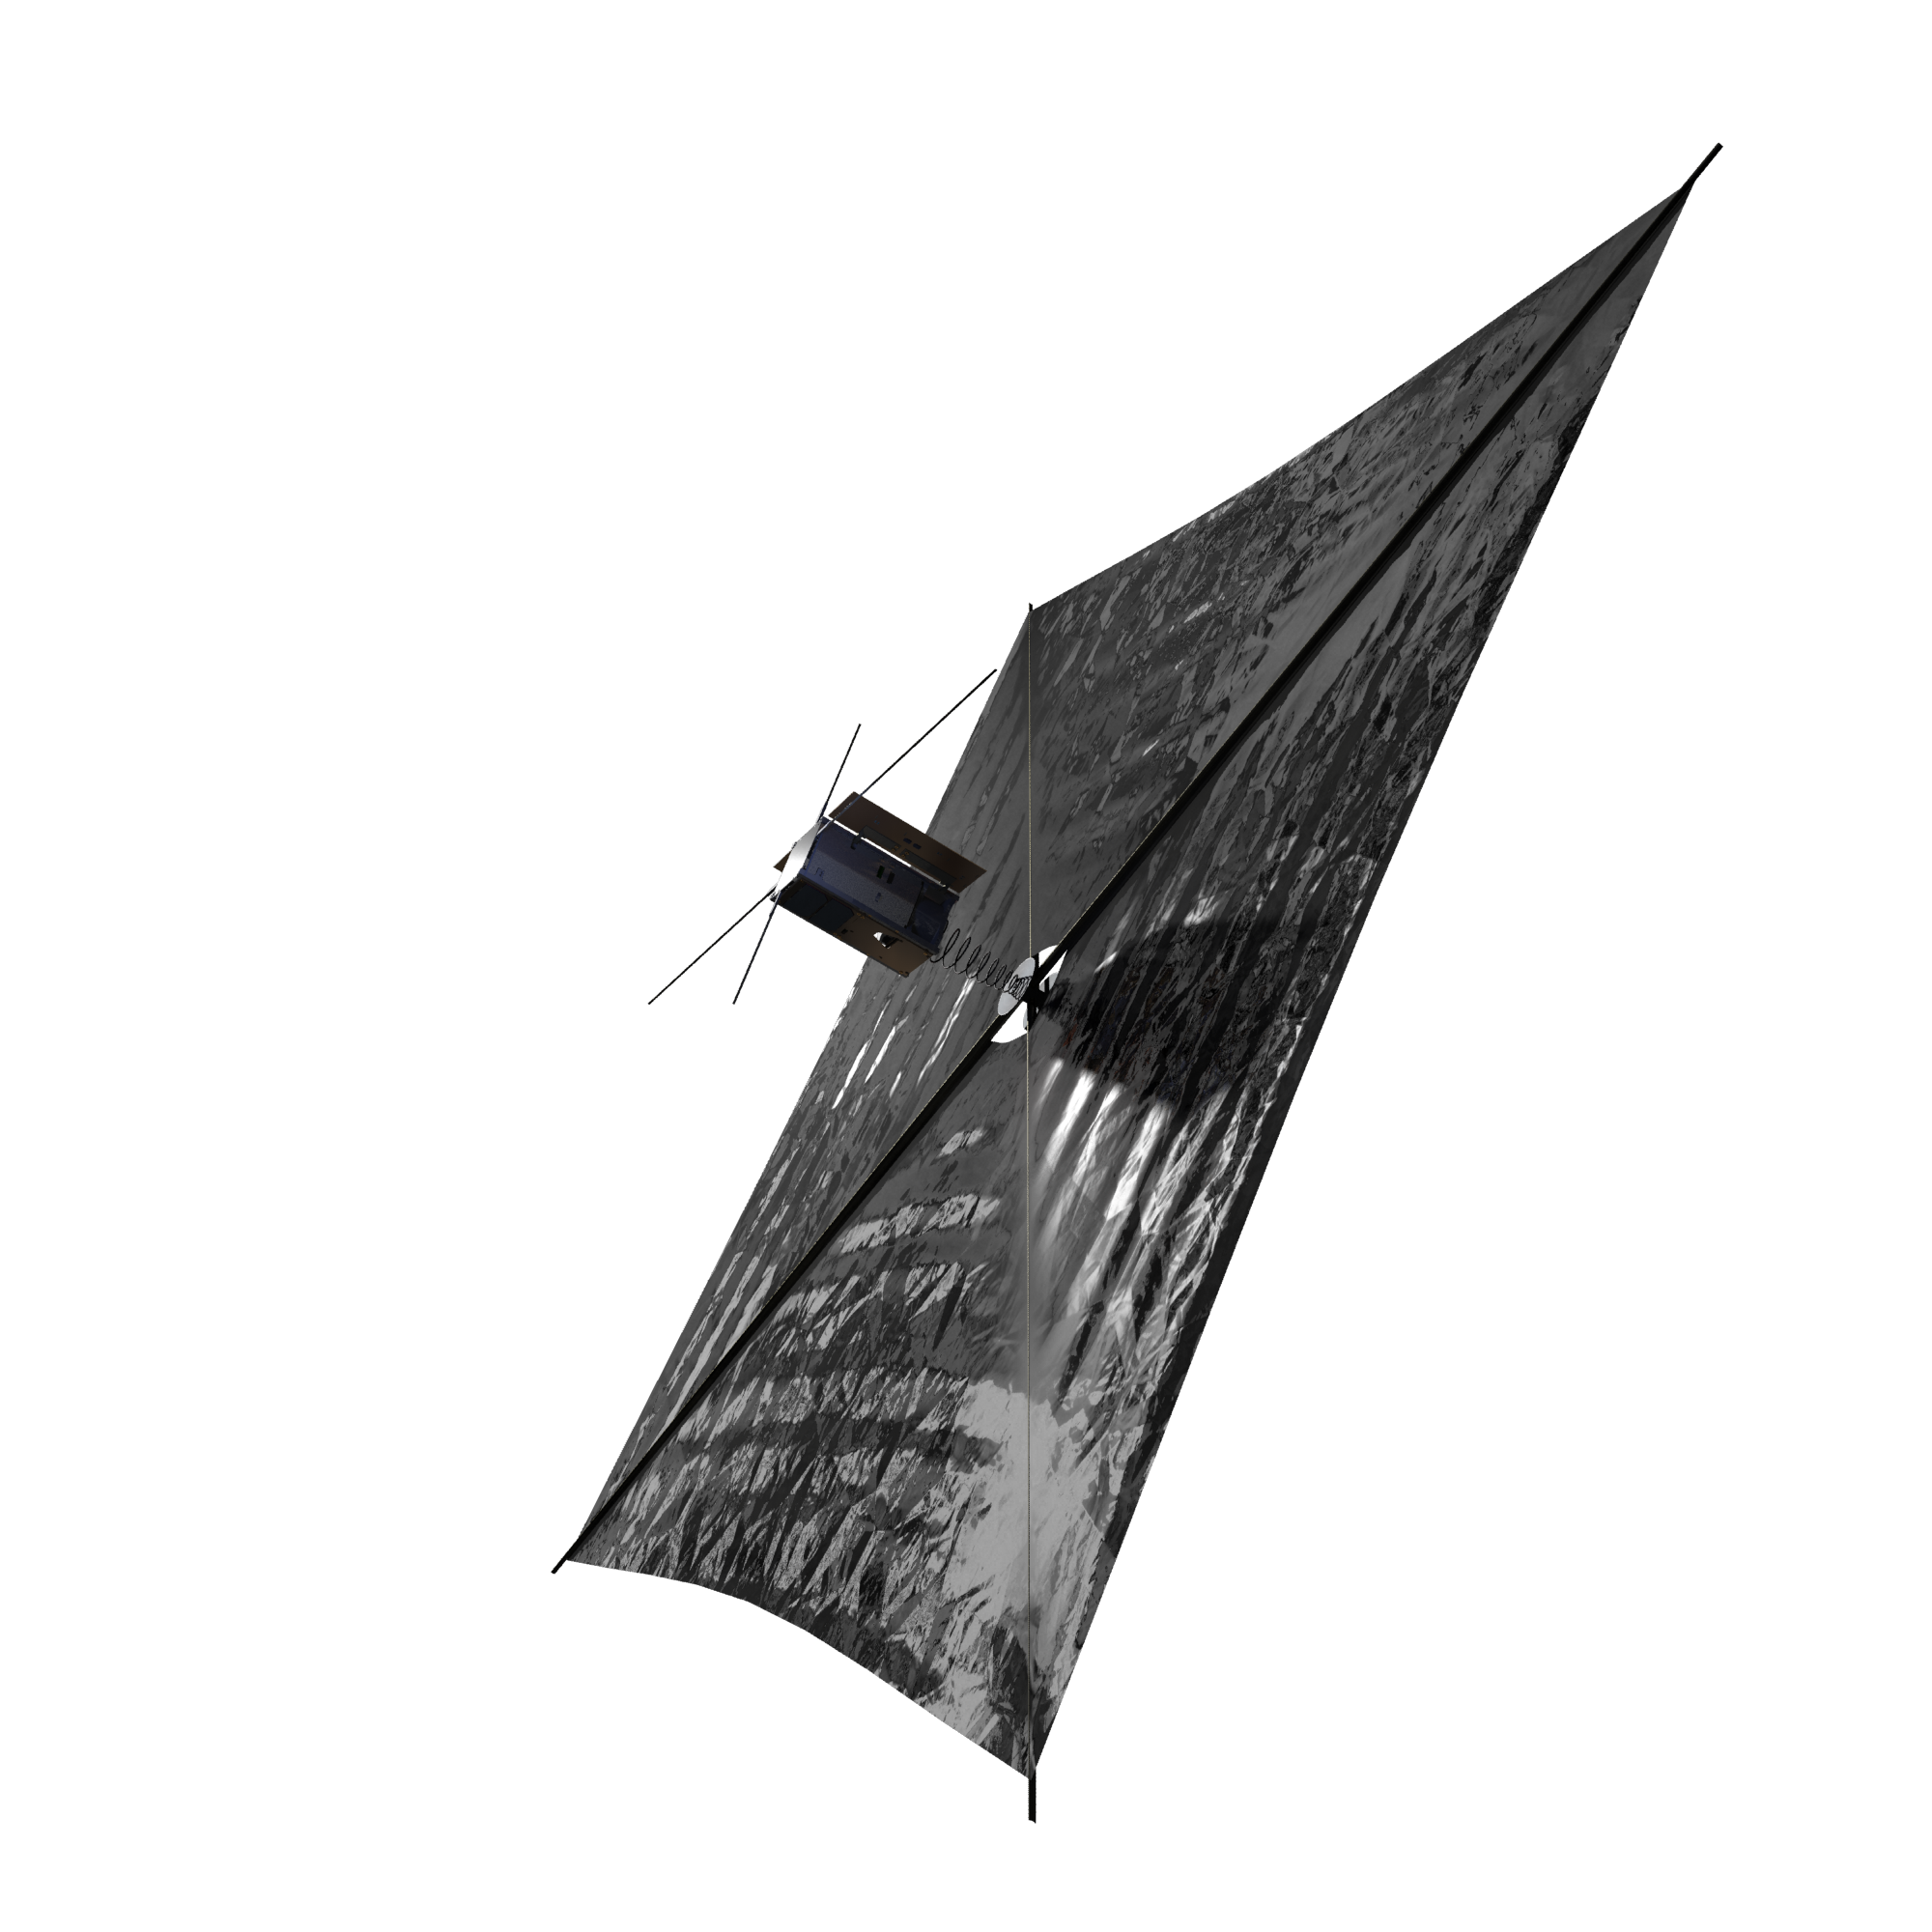
\includegraphics[width=0.7\paperwidth]{img/PW-Sat2_render_02.png}
        \caption{PW-Sat2 with opened sail (by M. Świetlik)}
        \label{PW-Sat_render_sail}
    \end{figure}

    More information about this experiment can be found in \cite{DDC_article}.

\subsection{Lifetime}
    Due to its primary mission PW-Sat2 lifetime is planned to be 40 days long. After this time deorbit sail will open, and orbit will slowly decrease. Deorbitation from nominal orbit is planned to take N days. Therefore sensor should be able to measure dose absorbed during full mission - N days.

\subsection{Orbit}
    PW-Sat2 in planned to be launched to sun-synchronous circular orbit of attitude \SI{575}{\kilo\meter}, with LTAN of $10:30$ \cite{PWSAT_MA_CDR}.


\subsection{Radiation analysis}
    Simulations in SPENVIS \cite{SPENVIS_URL} were performed to estimate TID accumulated during PW-Sat2 mission. On fig \ref{TIDvsSheilding} dose as a function of shielding thickness was plotted.

    \begin{figure}[H]
        \centering
        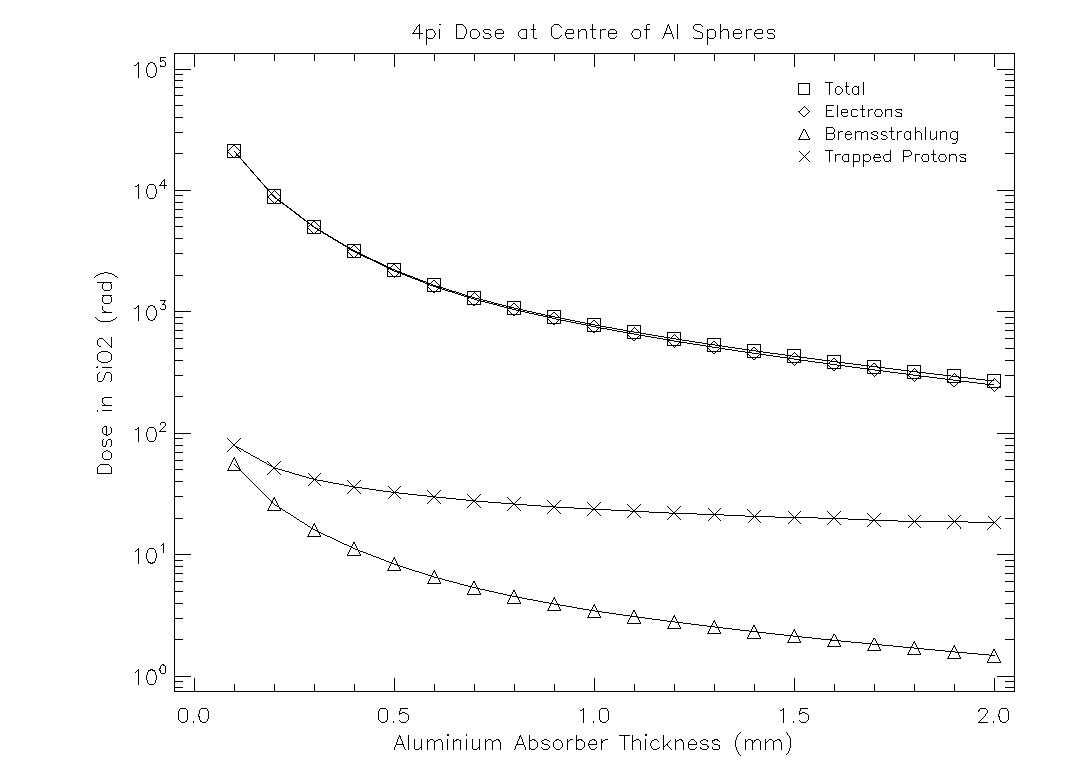
\includegraphics[width=0.7\paperwidth]{img/dose.eps}
        \caption{TID vs shielding}
        \label{TIDvsSheilding}
    \end{figure}

    Shielding of PW-Sat2 is about \SI{0.5}{\milli\meter} thick (aluminum sides as well as aluminum substrate for solar cells - \ref{PW-Sat_render_01}). Therefore predicted dose during PW-Sat2 mission is about \SI{10}{\kilo\rad}.


\section{Sensor requirements}
    Summing PW-Sat2 mission analysis, high-level sensor requirements were estimated:

    \begin{itemize}
        \item Total range of the sensor should be more than predicted dose. Derating this value gives range of about \SI{3}{\kilo\rad}.

        \item Resolution should be lower than \SI{0.1}{\kilo\rad}, 

        \item Total accuracy (across temperature \& component aging) should be less than \SI{0.5}{\kilo\rad}.
    \end{itemize}




\section{Applicable standards}
    The sensor should comply to ECSS \cite{ECSS_URL} standards. They are required by launch provider, as well as describing good practices during space product development.

    ESCIES \cite{ESCIES_URL} provide valuable knowledge about components qualifications, testing and verification.



\section{Electrical requirements}
    Sensor will be placed on-board of PW-Sat2. Therefore it should comply to its' standards - power supplies, communication interfaces etc.

\subsection{Electronics stack}
    Modules on PW-Sat2 are connected in PC-104 stack structure as shown on figure \ref{PW-Sat2_stack}. Is is placed inside structure and consists of (from the top):
    \begin{itemize}
        \item Payload module (PLD)
        \item On-Board Computer (OBC)
        \item Attitude Determination and Control Subsystem (ADCS)
        \item Electrical Power System (EPS)
        \item battery module (ACC)
        \item communication transceiver (COMM)
        \item antennas module (ANT)
    \end{itemize}

    \begin{figure}[H]
        \centering
        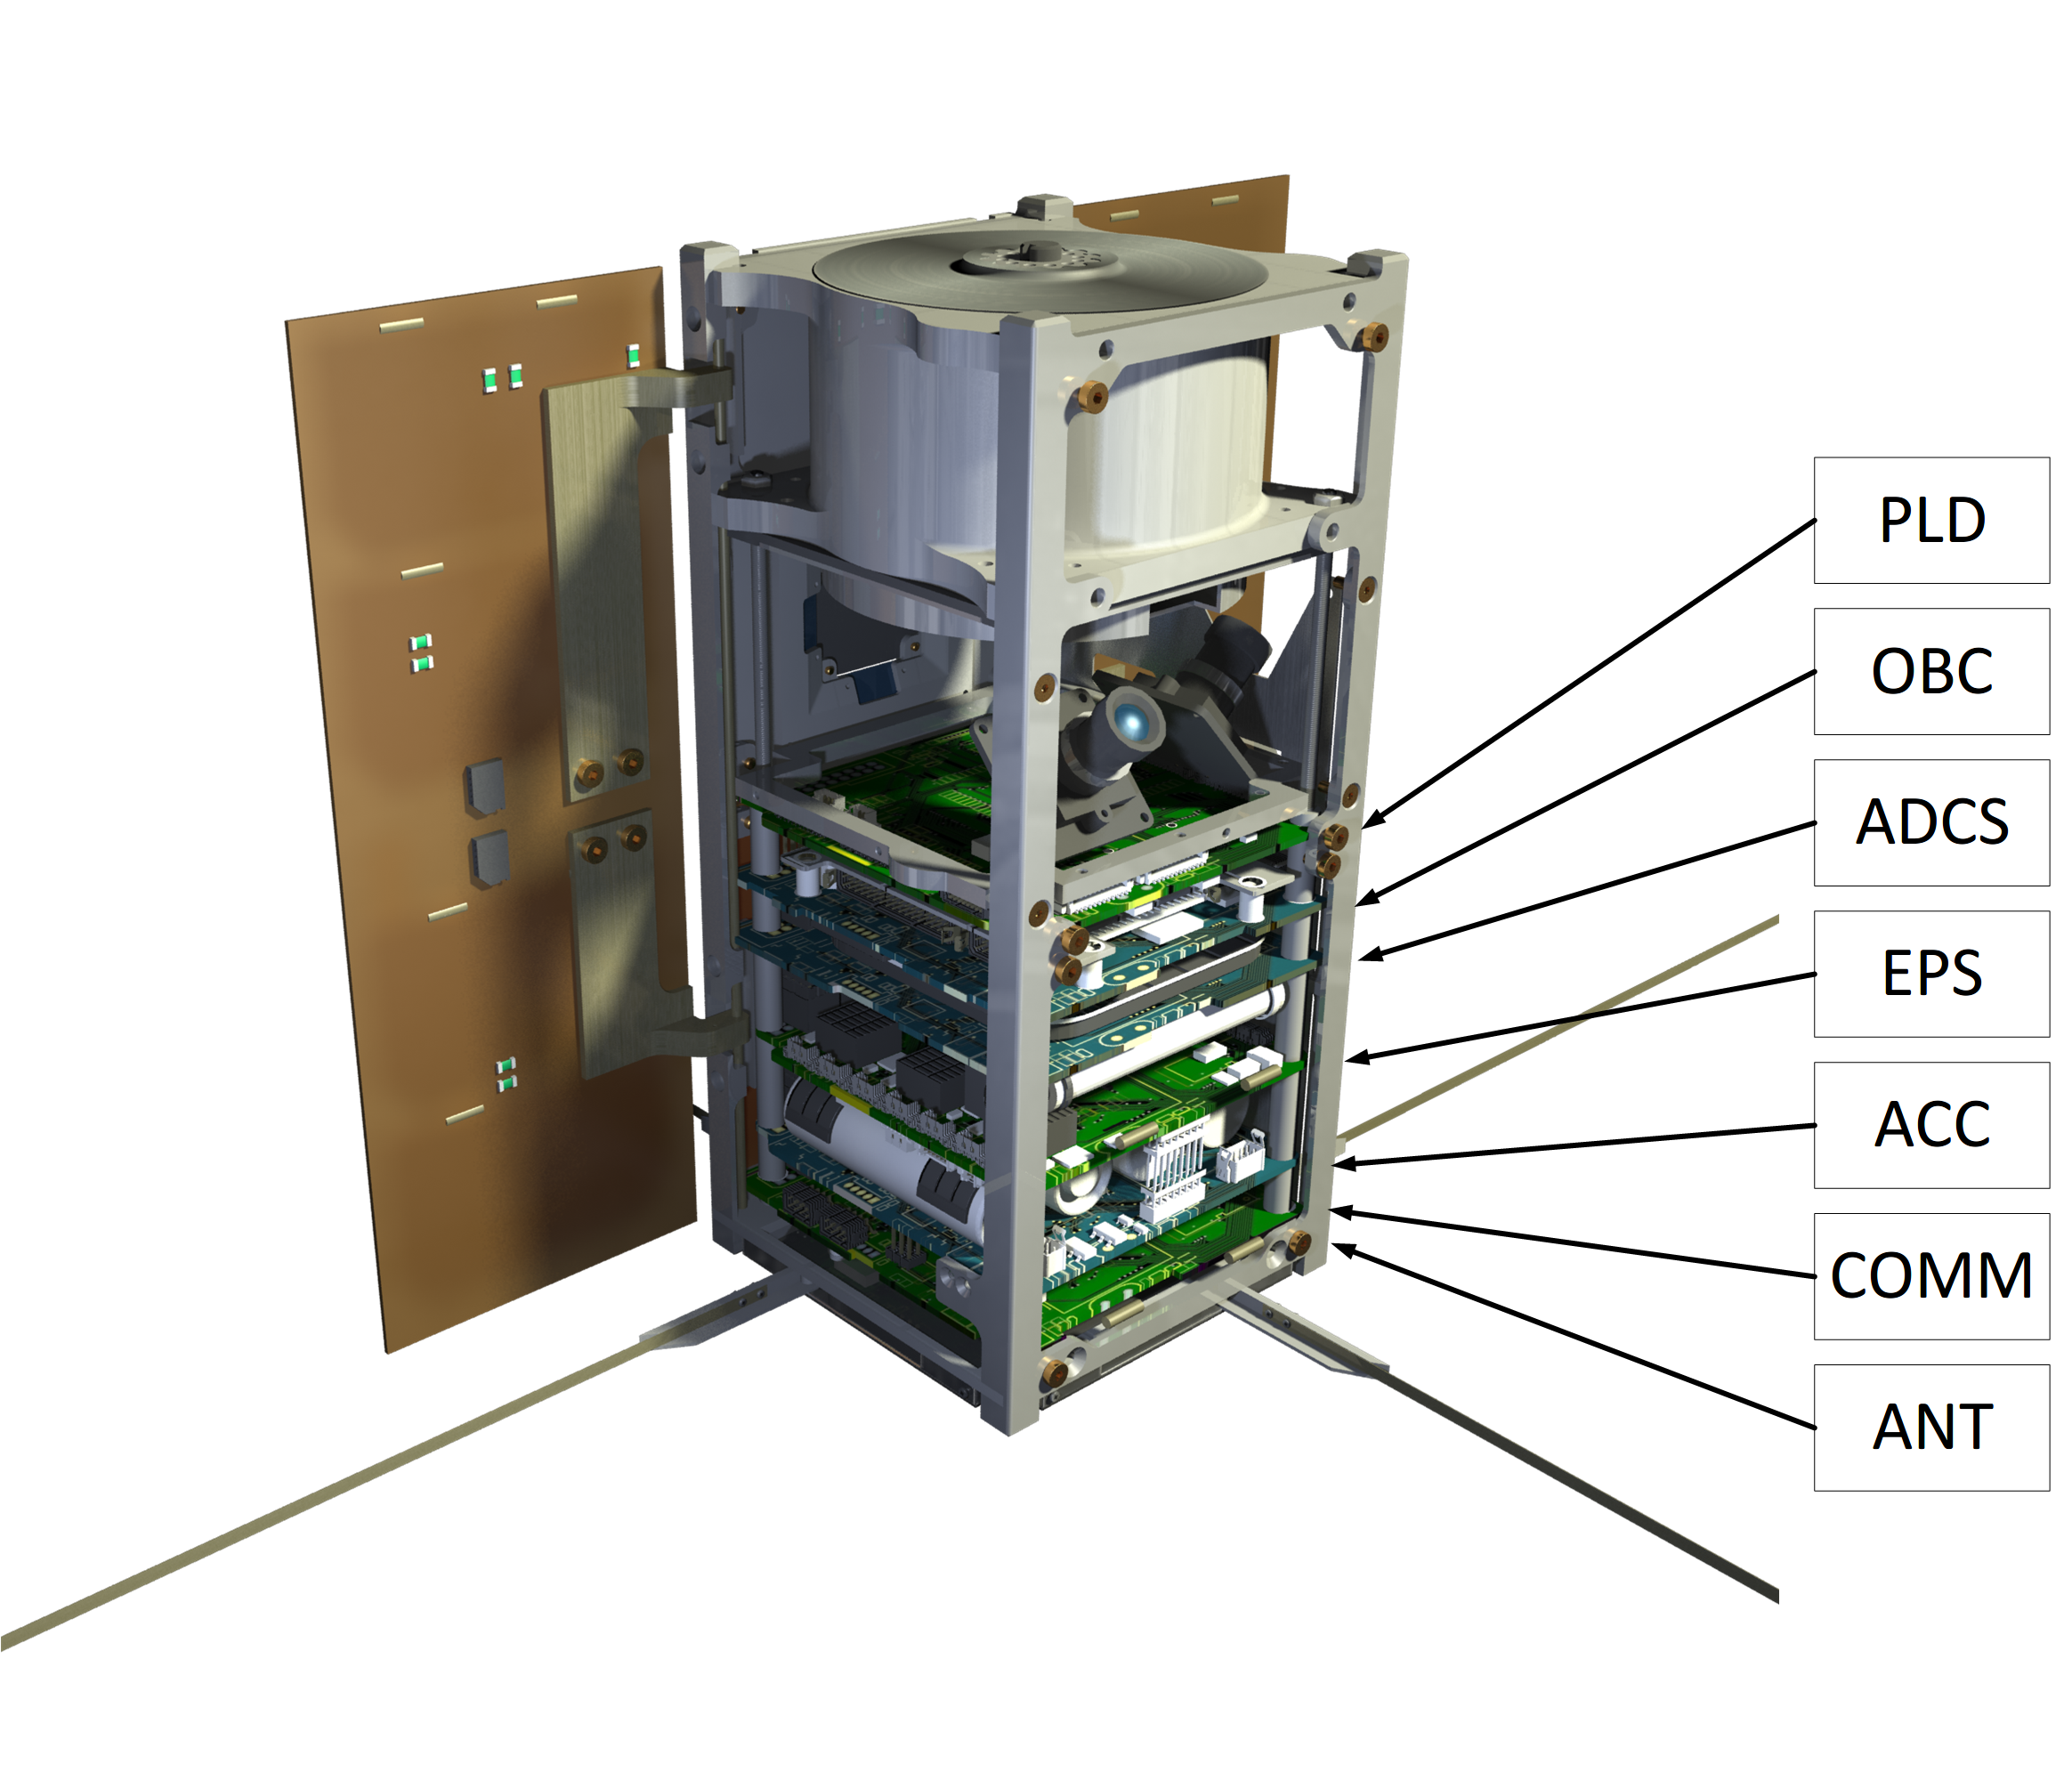
\includegraphics[width=0.7\paperwidth]{img/PW-Sat2-stack.png}
        \caption{PW-Sat2 electronics stack}
        \label{PW-Sat2_stack}
    \end{figure}


    Sensor will be placed on Payload board, on the top of PC-104 stack. It will be placed on its PCB, described in \ref{PCB_description}. It will be one of sensors on this board, connected to PC-104 stack.


\subsection{PC-104 connector}
    PLD board is connected to OBC with PC-104 connector. Pinout is shown on figure \ref{PC104_PLD}.

    \begin{figure}[H]
        \centering
        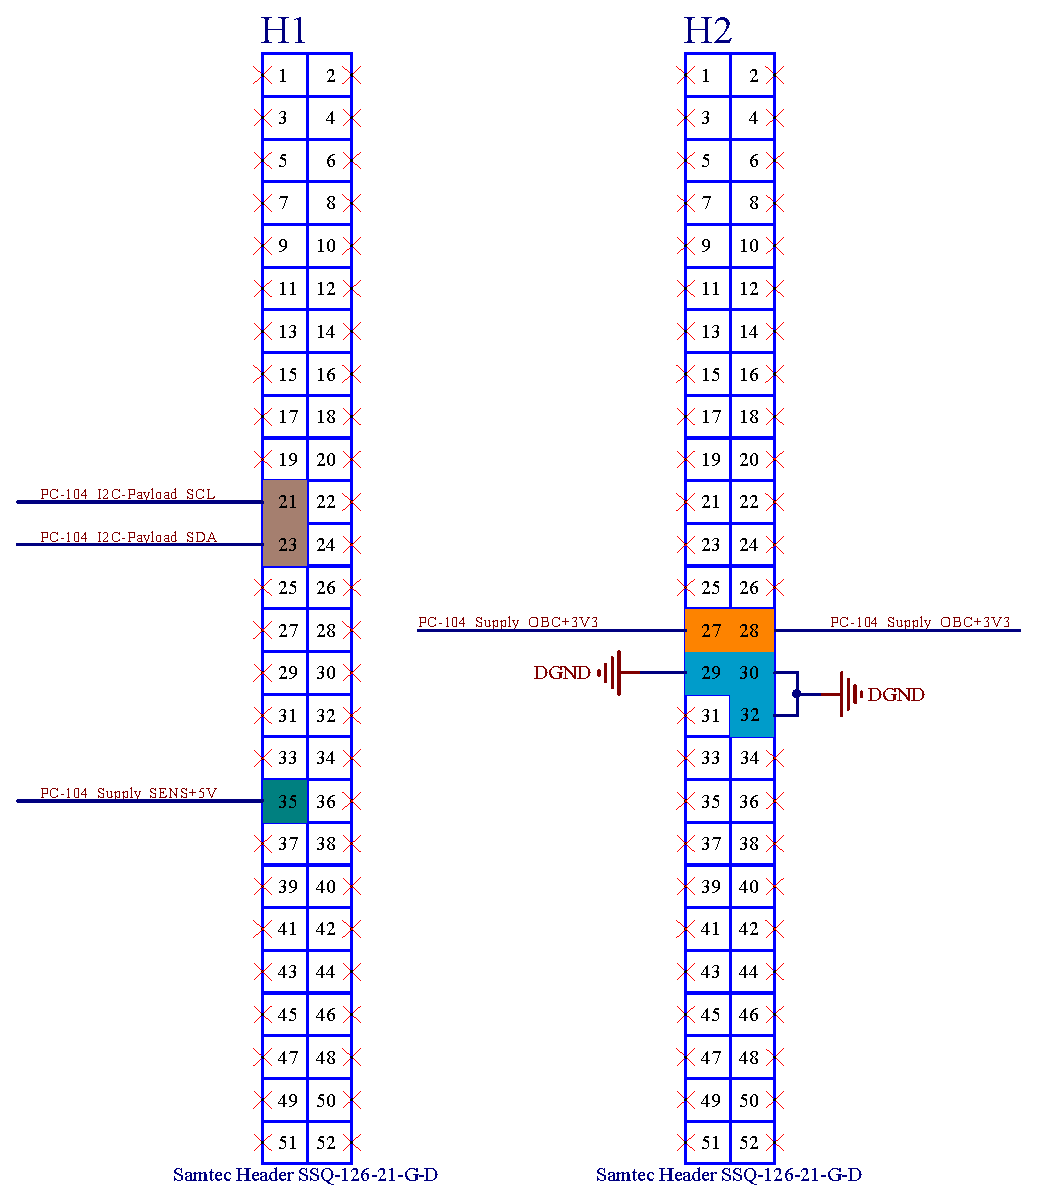
\includegraphics[width=0.5\paperwidth]{img/PC-104.eps}
        \caption{PC-104 connector to PLD board}
        \label{PC104_PLD}
    \end{figure}

    Connector consists of:
    \begin{itemize}
        \item $I^2C$ bus, connected directly to MCU on OBC
        \item SENS \SI{5}{\volt} line, powered when sensor is enabled by OBC
    \end{itemize}

\subsection{Power rail}
    As mentioned earlier, the power for the sensor is \SI{+5}{\volt}, activated whenever sensor should be accessed by OBC. 

    Power line is controlled and protected by Latchup-Current Limiter FPF2701MX placed on EPS board. Therefore additional latchup protection in not necessary in this design. However, this sensor will be not only one on PLD board and should have it's own power switch. PLD board is enabled and disabled by EPS on OBC command and sensor should be enabled only during TID readout. Having this in mind forces the design to be immune to immediate shutdowns. 

\subsection{Power consumption}
    During irradiation sensor should be completely turned off. It decreases possibility of radiation damage and increases overall system reliability.

    During readout required power should be less than \SI{1}{W}.

\subsection{Data interface}
    The sensor is connected to OBC via $I^2C$ interface. OBC on this bus is master - and sensor should be one of slaves. PLD board can be disabled, therefore it should provide isolation of $I^2C$ bus when it is powered off.

\subsection{Radiation immunity}
    Design should be itself immune to radiation. For PW-Sat2 threshold of \SI{10}{\kilo\rad} was chosen for all COTS components. Semiconductor components should have radiation as described in \cite{ESCIES_TID_test_method}.

\subsection{Electromagnetic compatibility}
    EMC requirements are described in \cite{ECSS_E_ST_20_07C}. This standard was tailored to PW-Sat2 because power rail is \SI{+5}{\volt}, other than on bigger S/C (\SI{+28}{\volt}).

    \begin{itemize}
        \item Conducted susceptibility is shown on figure \ref{EMC_conducted_susceptibility} . It was created by down-scaling figure A-4 from \cite{ECSS_E_ST_20_07C} by factor of $\SI{28}{\volt}/\SI{5}{\volt} = 5.6$. EMC limit on power line is defined as constant \SI{175}{\milli\volt} from \SI{30}{\hertz} to \SI{100}{\kilo\hertz}. Sensor should be able to filter this ripple to produce stable power for analog devices. In addition, it should be taken into account that output DC-DC converters on EPS runs on \SI{500}{\kilo\hertz}.

        \begin{figure}[H]
            \centering
            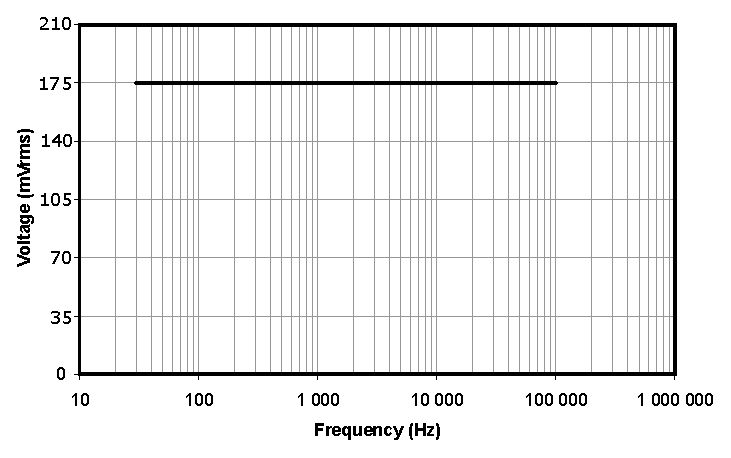
\includegraphics[width=0.5\paperwidth]{img/EMC_conducted_susceptibility.eps}
            \caption{Conducted susceptibility limit, frequency domain. Source: \cite{ECSS_E_ST_20_07C}}
            \label{EMC_conducted_susceptibility}
        \end{figure}


        \item Conducted emission is defined on figure \ref{EMC_conducted_emission}.

        \begin{figure}[H]
            \centering
            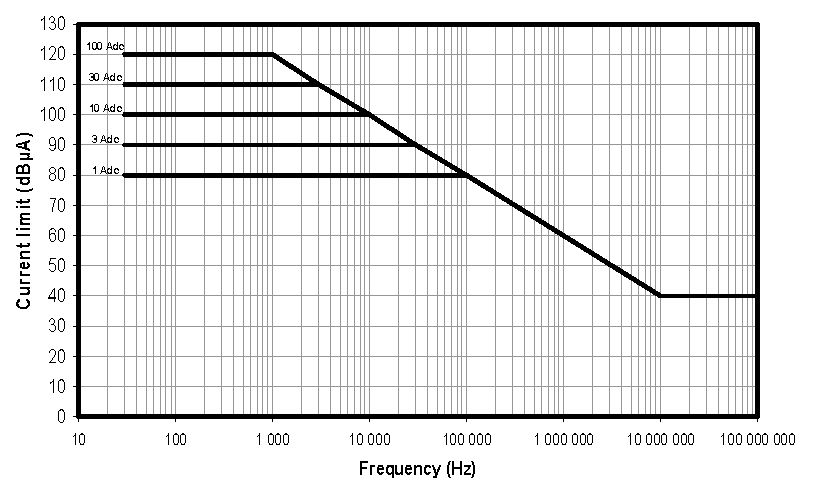
\includegraphics[width=0.5\paperwidth]{img/EMC_conducted_emission.eps}
            \caption{Conducted susceptibility limit, frequency domain. Source: \cite{ECSS_E_ST_20_07C}}
            \label{EMC_conducted_emission}
        \end{figure}    


        \item Radiated susceptibility.
            On board PW-Sat2 is a communication module transmitting \SI{0.5}{\watt} of power on frequency \SI{435.02}{\mega\hertz}. It is planned that during readout radio transmitter will be disabled, but proper tests should be conducted to check for possible errors and faults.

            PLD board is placed near OBC - so radiated emission from digital lines can couple to sensor elements causing noise and errors. Proper tests will be conducted and if necessary shielding will be implemented.

        \item Radiated emission.
            Sensor is not predicted to emit any kind of radio waves. In case of detected anomaly further design decisions would have to be made.

    \end{itemize}


\subsection{Inrush current}
    Inrush current have to be limited to maximum power consumption to not trigger LCL on EPS.

\subsection{Reliability of components}
    This sensor is not a critical part of the satellite. But, reliable components should be used to ensure proper results. 

    Every used component should have failure rate of $0.1\si{\percent}$ or lower. This is essential in capacitors and other passive components.


\section{Mechanical requirements}
    In this chapter design constrains and mechanical requirements of Falcon9 are presented. Launcher requirements were taken from \cite{Falcon9_user_manual}.

\subsection{PCB}
\label{PCB_description}
    PCB of PLD board is standard 4-layer FR4 board with stack shown on figure \ref{PLD_PCB_stack}. Its dimensions are shown on \ref{PLD_PCB_size}, but design is forced to take much less space. For this sensor limits are \SI{3x3}{\centi\meter} double sided.

    \begin{figure}[H]
        \centering
        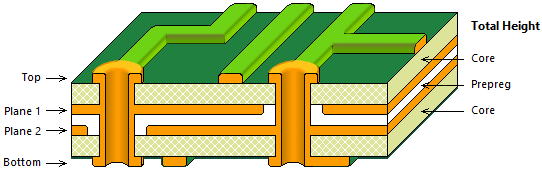
\includegraphics[width=0.5\paperwidth]{img/PLD_PCB_stack.png}
        \caption{PLD board PCB stack}
        \label{PLD_PCB_stack}
    \end{figure}    

    \begin{figure}[H]
        \centering
        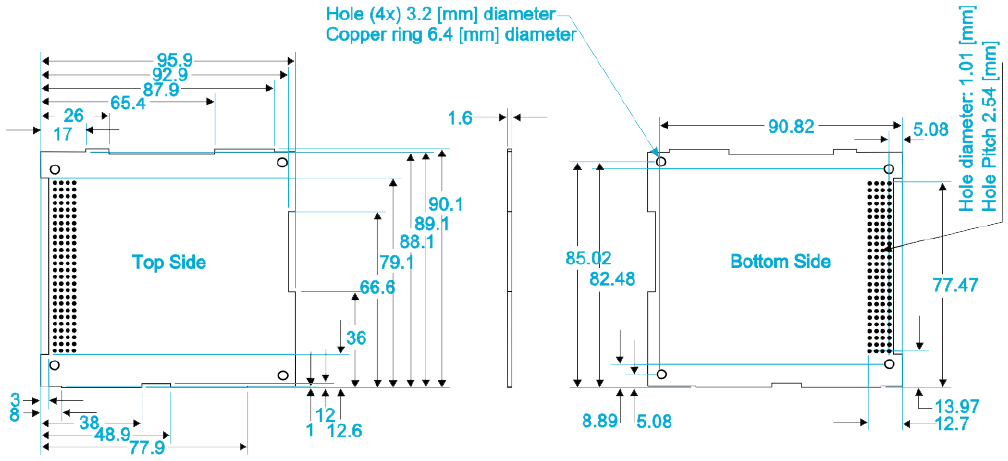
\includegraphics[width=0.7\paperwidth]{img/PC104_PLD_size.png}
        \caption{PC-104 size}
        \label{PLD_PCB_size}
    \end{figure}    



\subsection{Outgassing}
    Every used component should be able to work in vacuum. Outgassing of components should be known to conduct required vacuum tests before launch.

\subsection{Vibration}
    During rocket launch large vibrations occur on payload, therefore it should be immune to it. In case of any heavy electronic components appropriate glue should be applied to prevent joint cracks.
    \begin{figure}[H]
        \centering
        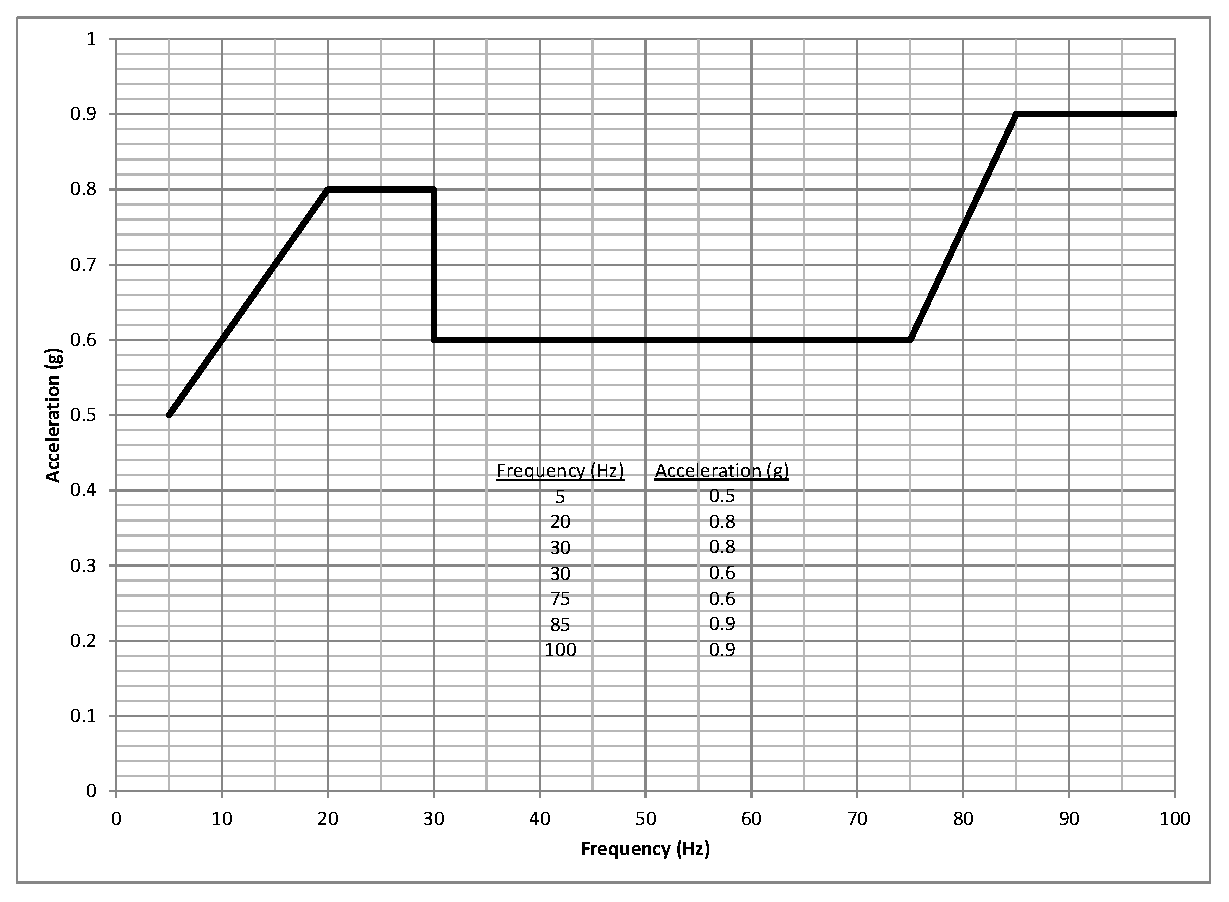
\includegraphics[width=0.5\paperwidth]{img/Falcon9_vibration.eps}
        \caption{Falcon9 maximum axial equivalent sine environment. Source: \cite{Falcon9_user_manual}}
        \label{Falcon9_vibration}
    \end{figure}    


\subsection{Operation temperature}
    The sensor should work in every operational case satellite can be. Simulations were performed to find bounds of possible temperature range inside satellite.    In \cite{PWSAT_TCS_CDR} results are presented. 

    For PLD board operation range is $\SI{0}{\degreeCelsius}$ to $\SI{60}{\degreeCelsius}$. If the measured temperature will be outside this region, sensor will not be enabled.


\subsection{Thermal cycles}
    Or PW-Sat2 orbit sun illumination is changing every $\approx \SI{90}{\minute}$. Therefore large number of thermal cycles are applied to On-Board electronics, which can cause joint cracks as well as component failures. Proper soldering and component selection will be made, according to ECSS.

    As described in \cite{ECSS_Q_ST_70_04C} the sensor should pass thermal cycle tests: $100$ times from $- (100 \pm 5)$\si{\degreeCelsius} to $(100 \pm 5)$\si{\degreeCelsius} in vacuum environment. Test procedure is shown on \ref{thermal_tests}.

    \begin{figure}[H]
        \centering
        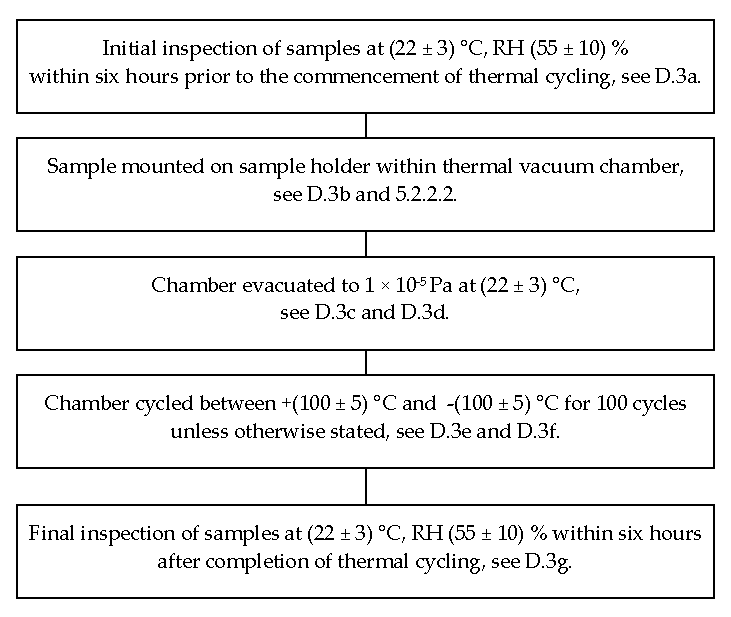
\includegraphics[width=0.5\paperwidth]{img/thermal_cycles.eps}
        \caption{Thermal cycles test procedure. Source: \cite{ECSS_Q_ST_70_04C}}
        \label{thermal_tests}
    \end{figure}

\chapter{Sensor design}
This chapter will cover sensor basics, sensing element selection and theory of operation. The design will be presented at a system-level view. For a more detailed description of the electronics, please skip to chapter \ref{Engineering_model_chapter}.

\section{Review of commercially available RadFETs}
    Commercial solutions are based on a modified MOS structure (with thicker gate region). Example silicon structure is shown in the figure \ref{Tyndall_radfet_silicon}. Different companies produce their own RadFET devices, by designing individual structures fitted to particular requirements. Researched companies only produce the RadFET sensors, leaving the readout circuit design for the customer to realise. A physical schematic and description for RadFET sensors is found in section \ref{Radiation_effects_on_MOS_transistors}. In the table \ref{commercial_radfet_comparison} commercially available RadFETs are compared.

    \begin{figure}[H]
        \centering
        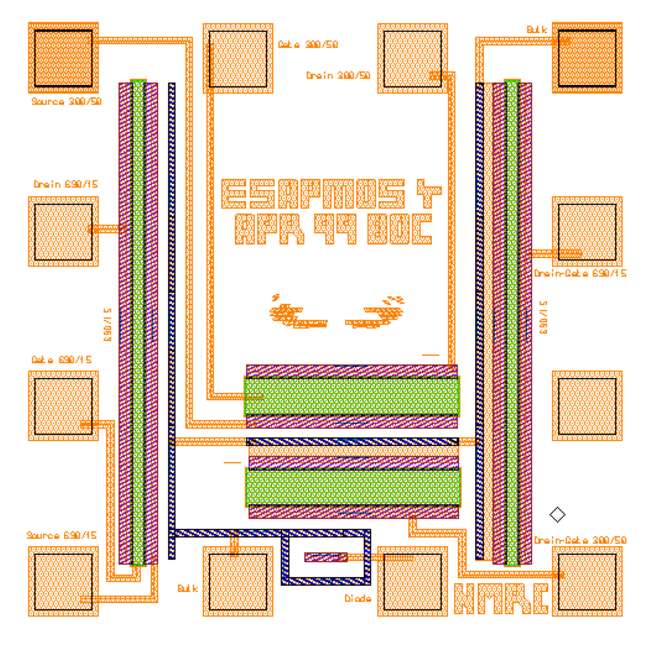
\includegraphics[width=0.45\paperwidth]{img/05/radfet-silicon.eps}
        \caption{4x RadFET silicon structure by Tyndall. Source: \cite{Tyndall_Radfet}}
        \label{Tyndall_radfet_silicon}
    \end{figure}

    \begin{table}[H]
    \caption{Commercial RadFET comparison}
    \label{commercial_radfet_comparison}
    \begin{tabular}{| L{3.5cm} | C{3.5cm} | C{3.5cm} | C{3.5cm} |}
        \hline
        Type: & REM RFT300 & Tyndall TY1003 & Tyndall TY1004 \\ \hline

        Image: &
        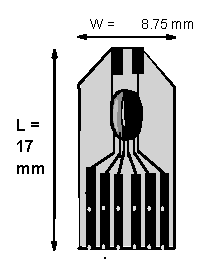
\includegraphics[width=0.10\paperwidth]{img/05/rem.eps} &
        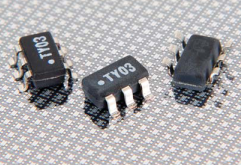
\includegraphics[width=0.15\paperwidth]{img/05/TY1003.png} &
        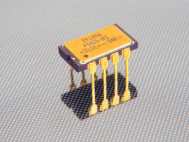
\includegraphics[width=0.15\paperwidth]{img/05/TY1004.png} \\ \hline

        Package: & custom & SOT23-6 & 8-pin ceramic DIL \\ \hline

        \# of transistors: & 2 & 2 & 2 \\  \hline

        Recommended readout current: & $10$ - \SI{500}{\micro\ampere} & \multicolumn{2}{c|}{\SI{10}{\micro\ampere}} \\ \hline

        TID dependency: & $n = 1$, $A~=~0.117$~\si{\milli\volt/\rad} & $n = 0.46$, $A~=~29.5$~\si{\milli\volt/\rad} & $n = 0.41$, $A~=~65.6$~\si{\milli\volt/\rad} \\ \hline
        Temperature readout: & diode & diode & diode \\ \hline
    \end{tabular}
    \end{table}


\section{COTS MOSFET as RadFET}
    RadFETs are specifically designed MOSFETs that act as radiation sensors. However, the parameters of COTS MOSFET transistors also depend on total absorbed dose. They are much cheaper, but require proper calibration and testing in order to be considered as a flight solution.

    Many articles and papers prove that COTS MOSFETs can be used reliably as TID sensors. A number of available transistors were tested, their basic characteristics are compared in the table \ref{cots_mosfet_comparison}. Parameters are taken at unbiased gate.

    \begin{table}[H]
    \caption{COTS MOSFET comparison}
    \label{cots_mosfet_comparison}
    \begin{tabular}{| L{2cm} | C{2.4cm} | C{2.4cm} | C{2.4cm} | C{2.4cm} | C{2.4cm} |}
        \hline
        Type: & 3N163 & ZVP3306 & ZVP4525 & BS250F & CD4007 \\ \hline
        Reference: & \cite{3N163_article} & \cite{COTSMosfetsGarcia} & \cite{COTSMosfetsGarcia} & \cite{COTSMosfetsGarcia} & \cite{COTSMosfetsGarcia} \\ \hline

        Package: & TO-72 & TO-92 & SOT-223 & SOT-23 & TSSOP-14 \\ \hline

        $I_{ZTC}$ [\si{\micro\ampere}]: & 225 & - & - & - & 145 \\ \hline

        Sensitivity [\si{\milli\volt/\gray}]: & $24.3\pm 1.8$ & $3.7\pm 0.3$ & $3.4\pm 0.4$ & $3.1\pm 0.4$ & $4.6\pm 0.1$ \\ \hline

        $V_{TH_0} [\si{\volt}]$: & $2.0 - 3.0$ & $2.0 - 3.0$ & $1.5 - 2.5$ & $2.5 - 3.5$ & $1.9 - 2.5$ \\ \hline

        $V_{TH}$ @ \SI{100}{\gray} [\si{\volt}]: & $5.61$ & $3.4$ & $2.88$ & $3.85$ & $2.97$ \\ \hline
    \end{tabular}
    \end{table}

    3N163 type have the greatest sensitivity - but bearing in mind the \SI{5}{\volt} supply for the sensor, it was discarded for too small range. The second best type is CD4007, which was selected for testing. Its parameters are suitable for the use under discussion, as shown in the table \ref{CD4007_parameters}.

    Other advantages of CD4007 are:
    \begin{itemize}
        \item 3 P-MOS in one package - averaging/redundancy,
        \item additional diodes and transistors in device - possible temperature measurement
        \item small, vibration and thermally resistant package
    \end{itemize}

\section{Selected MOSFET - CD4007}
    The CD4007 consists of three complementary pairs of N- and P-channel enhancement mode MOS transistors. Internal connection diagram is shown below in the figure \ref{CD4007_internal_diagram}. Predicted parameters of those transistors are collected in the table \ref{CD4007_parameters}.

    \begin{figure}[H]
        \centering
        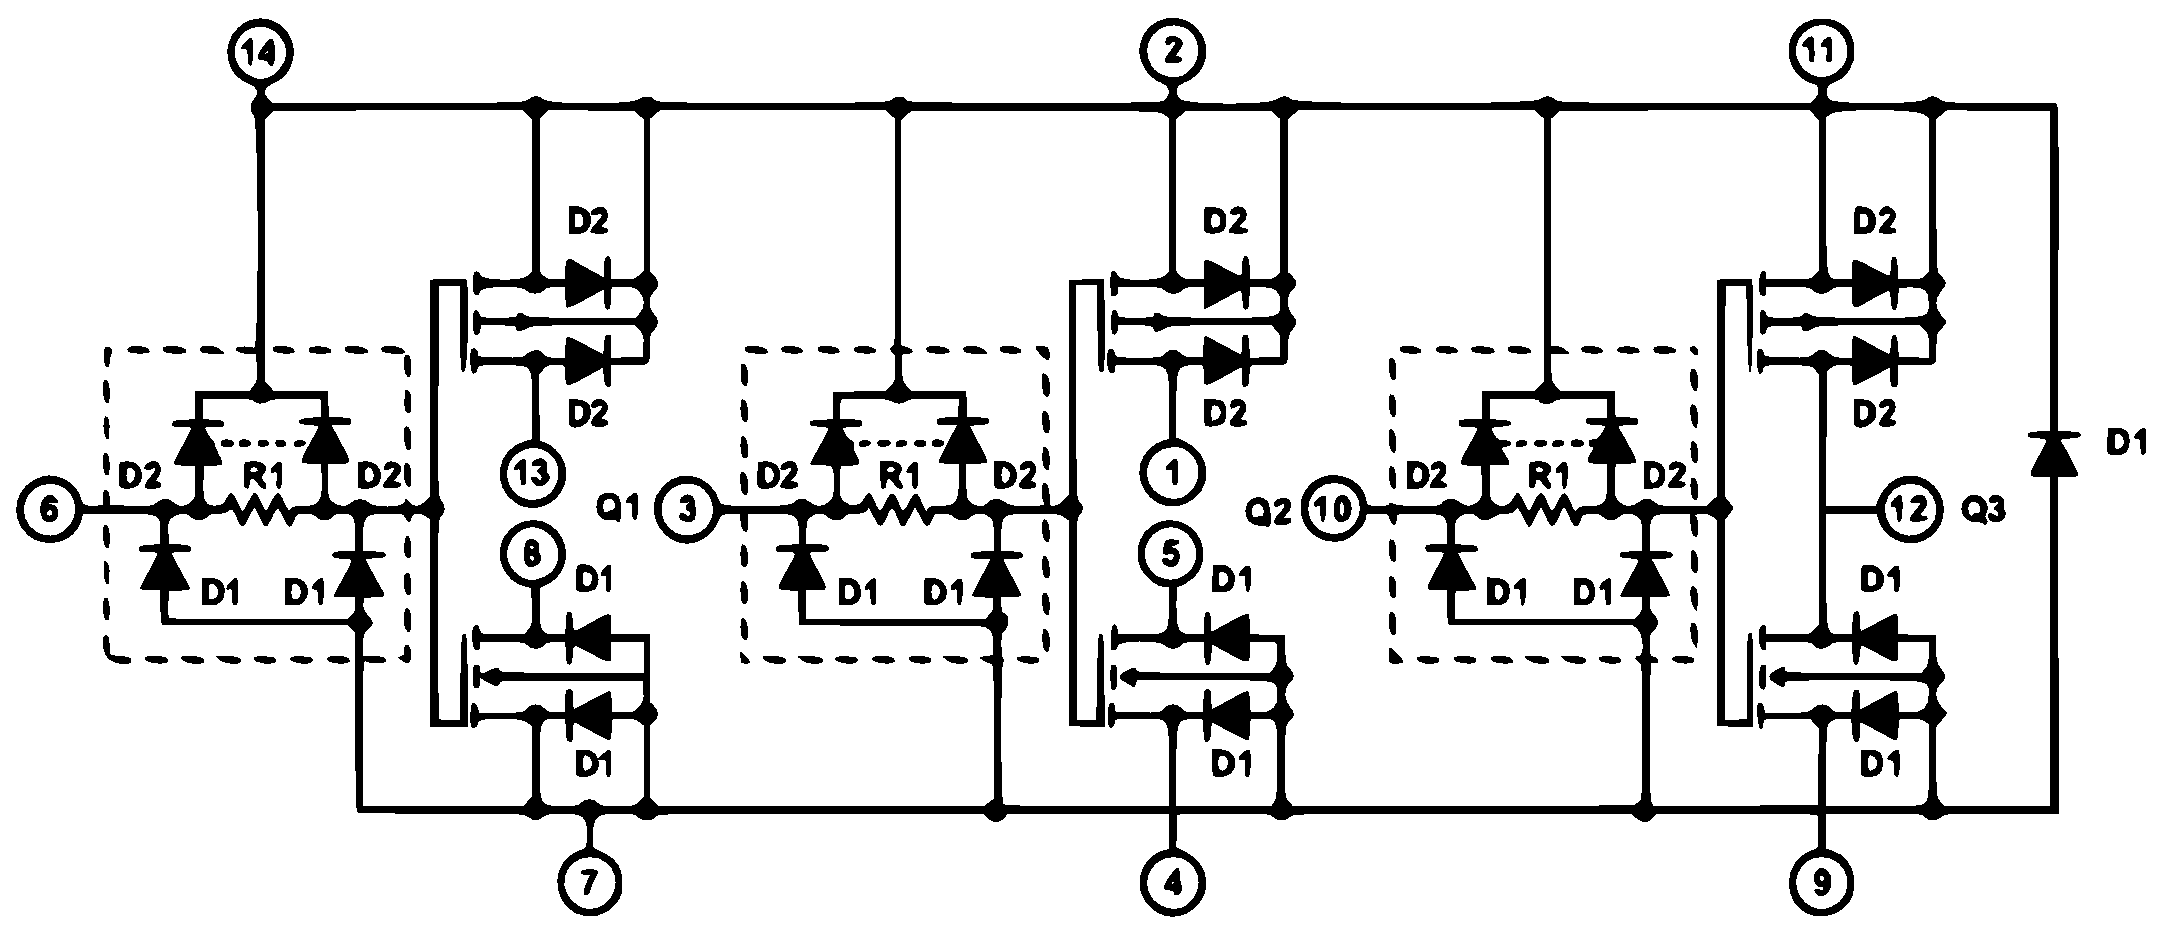
\includegraphics[width=0.7\paperwidth]{img/05/cd4007.eps}
        \caption{CD4007 internal diagram. Source: \cite{CD4007_schematic_functional}}
        \label{CD4007_internal_diagram}
    \end{figure}

    \begin{table}[H]
    \caption{CD4007 parameters}
    \label{CD4007_parameters}
    \begin{tabular}{R{7cm} | L{7cm} }
        Transistor type: & 3x P-MOS and 3x N-MOS \\ \hline
        Supply voltage: & 3-18~\si{\volt} \\ \hline
        Threshold voltage: & \SI{1.8}{\volt} @ \SI{100}{\micro\ampere} \\ \hline
        Temperature range: & \SI{-55}{\degreeCelsius} - \SI{125}{\degreeCelsius} \\ \hline
        Zero-temperature coefficient current: & \SI{140}{\micro\ampere} \\ \hline
        Predicted sensitivity: & \SI{4.6}{\milli\volt/\gray}
    \end{tabular}
    \end{table}

\section{Threshold voltage measurement}
    Threshold voltage changes with TID accumulated. The easiest method to measure change of this parameter is to connect the MOSFET in diode configuration, forcing constant drain current. A block diagram of this method is shown in the figure \ref{Vth_readout_block_diagram}.

    \begin{figure}[H]
        \centering
        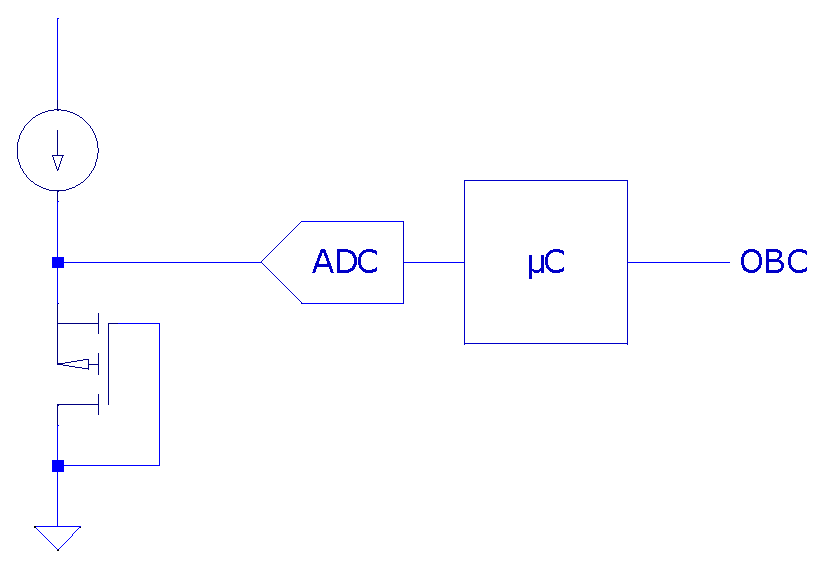
\includegraphics[width=0.3\paperwidth]{img/05/conceptual_block_diagram.eps}
        \caption{Threshold voltage readout block diagram}
        \label{Vth_readout_block_diagram}
    \end{figure}

    In saturation region, drain current is described by the following equation (body effect is negligible):

    $$I_D = A \cdot (V_{GS} - V_{th})^2$$
    Where:

    \begin{tabular}{lcl}
        $I_D$ & - & drain current \\
        $A = \frac{\mu_n C_{ox}}{2} \frac{W}{L}$ & - & constant for partuicular transistor \\
        $V_{GS}$ & - & gate-source voltage \\
        $V_{th}$ & - & threshold voltage \\
    \end{tabular}
    \bigskip

    Because only the threshold voltage change is of interest, measuring $V_{GS}$ has the same effect:
    $$I_D = A \cdot (V_{GS_1} - V_{th_1})^2 = A \cdot (V_{GS_2} - V_{th_2})^2$$
    $$\Delta V_{GS} = \Delta V_{th}$$

    The sensor should be shut down during irradiation - therefore no-bias method was used. It allows for complete isolation of supply power to the sensor, enabling it only for readout.

\section{Temperature measurement}
    Because threshold voltage strongly depends on die temperature, this effect has to be compensated for. The flight MOSFET will be calibrated in a thermal chamber prior to launch, thus obtaining characteristic curves.

    A number of possible temperature measurement techniques were considered during this thesis:
    \begin{table}[H]
    \caption{Temperature readout methods}
    \begin{tabular}{C{4.5cm} | C{5cm} | C{5cm} }
        \textbf{Method} & \textbf{Pros} & \textbf{Cons} \\ \hline

        PT-1000 sensor glued to MOSFET & accurate reading & large thermal resistance, difficult assembly, low reliability \\ \hline

        ESD diode measurement in CD4007 & no additional sensor & complicated current, multiplexing circuit, unknown characteristics \\ \hline

        body diode in N-MOSFET in CD4007  & simple setup, reliable, known characteristics, low thermal resistance & no possibility of simultaneous readout of threshold and temperature (short thermal lag)
    \end{tabular}
    \end{table}

    The chosen solution: to measure temperature of silicon die using body diode in complementary N-MOS transistor. A block diagram of this proposed solution is presented in the figure \ref{Temperature_measurement_block_diagram}.

    \begin{figure}[H]
        \centering
        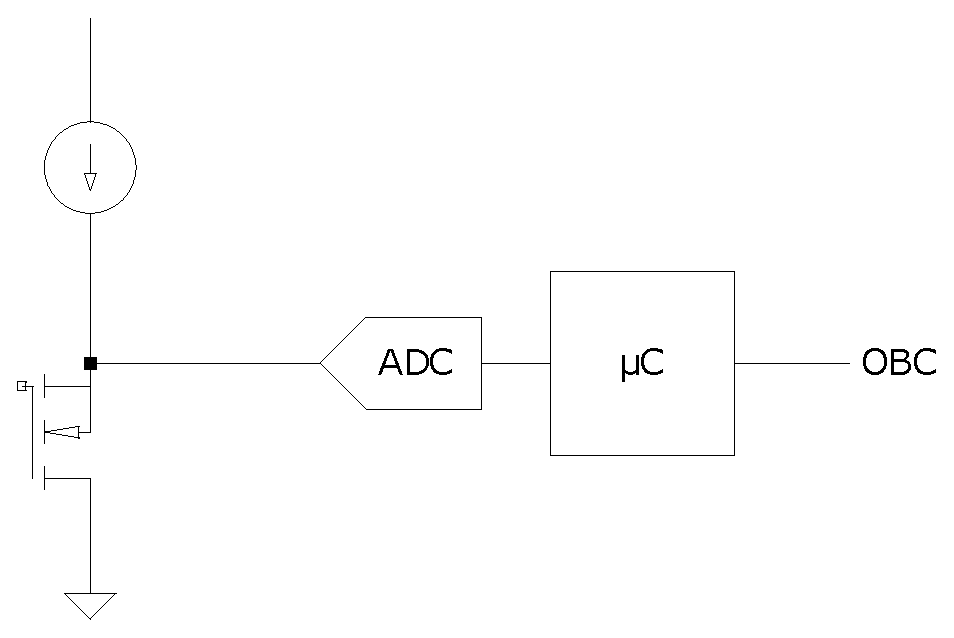
\includegraphics[width=0.5\paperwidth]{img/05/n-mos-temperature.eps}
        \caption{Temperature measurement block diagram}
        \label{Temperature_measurement_block_diagram}
    \end{figure}

    During calibration, both the temperature characteristics of the diode and the p-MOS threshold voltage will be obtained. They will be used to compensate for the threshold voltage shift associated with temperature. An individual flight component will be placed in a thermal chamber, and a proper look-up table will be created, with possible polynomial approximation.

\newpage
\section{Characteristic curves}
\label{Characteristic_curves}

    During M. Gumiela's thesis, \cite{MGThesis} a calibration stand for CD4007 was developed. As an outcome of that project, rough calibration curves were obtained, which are presented below.

    \bigskip \textbf{p-MOSFET transfer characteristics}
    \begin{figure}[H]
        \centering
        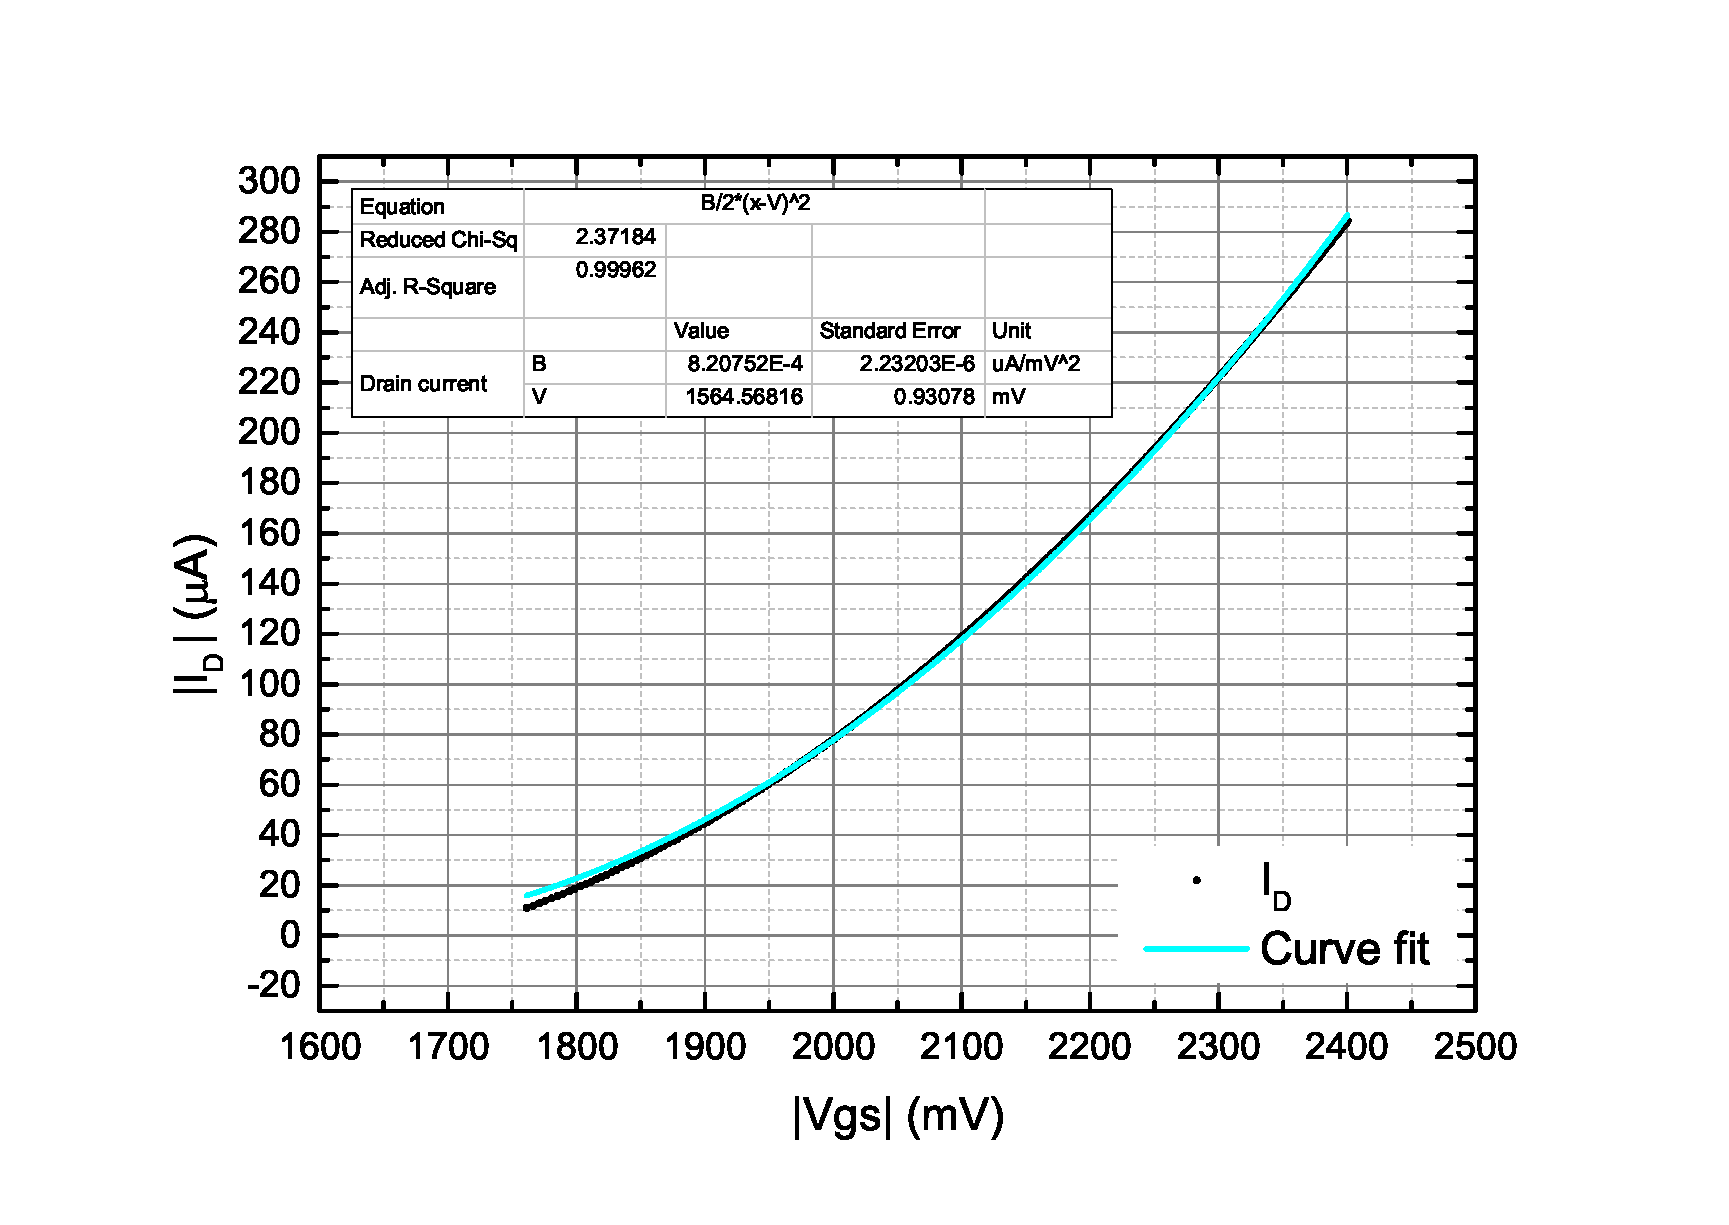
\includegraphics[width=0.56\paperwidth]{img/05/mg_iv_mosfet.eps}
        \caption{CD4007 p-MOSFET transfer characteristics. Source: \cite{MGThesis}}
        \label{CD4007_p-MOSFET_transfer}
    \end{figure}

    \bigskip \textbf{Linearized temperature coefficient of threshold voltage}
    \begin{figure}[H]
        \centering
        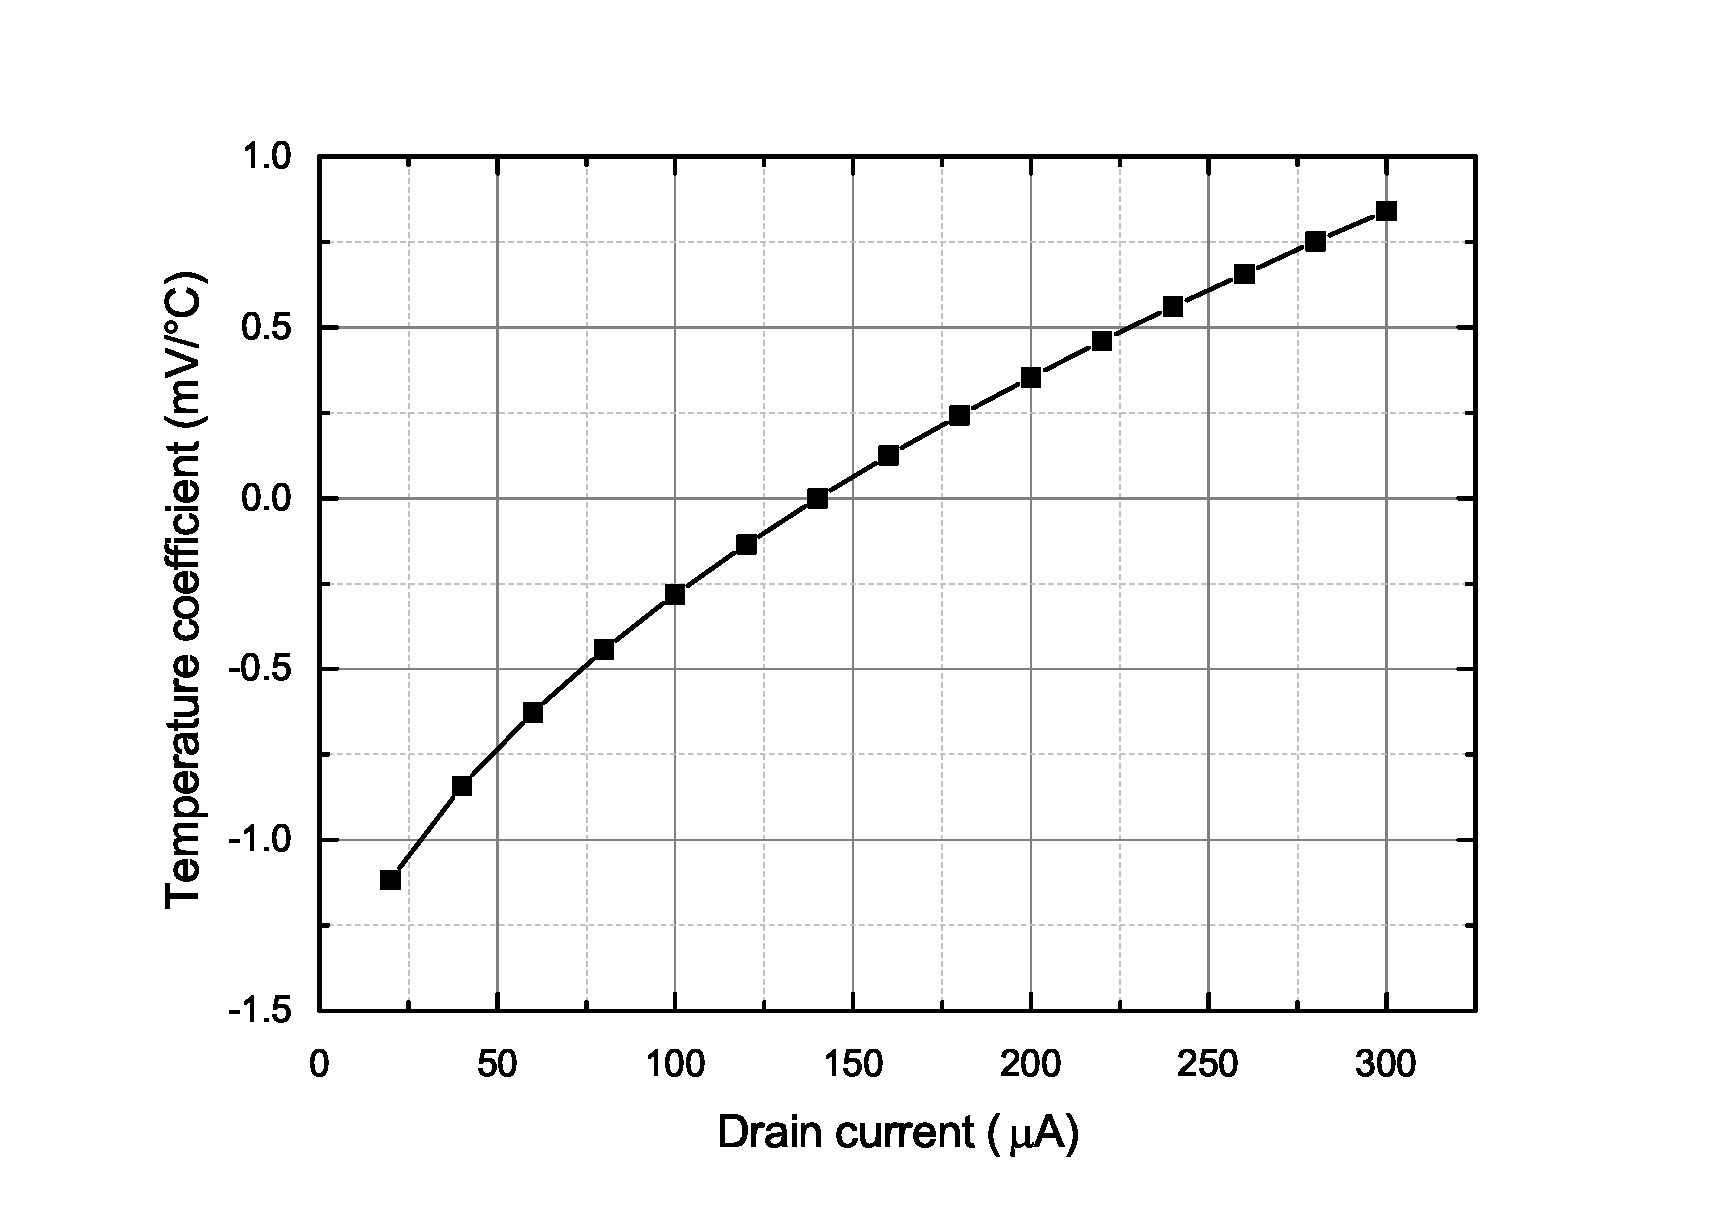
\includegraphics[width=0.56\paperwidth]{img/05/mg_tc_coefficients.eps}
        \caption{Linearized temperature coefficient of threshold voltage. Source: \cite{MGThesis}}
    \end{figure}

    \bigskip \textbf{Body diode forward voltage temperature calibration}
    \begin{figure}[H]
        \centering
        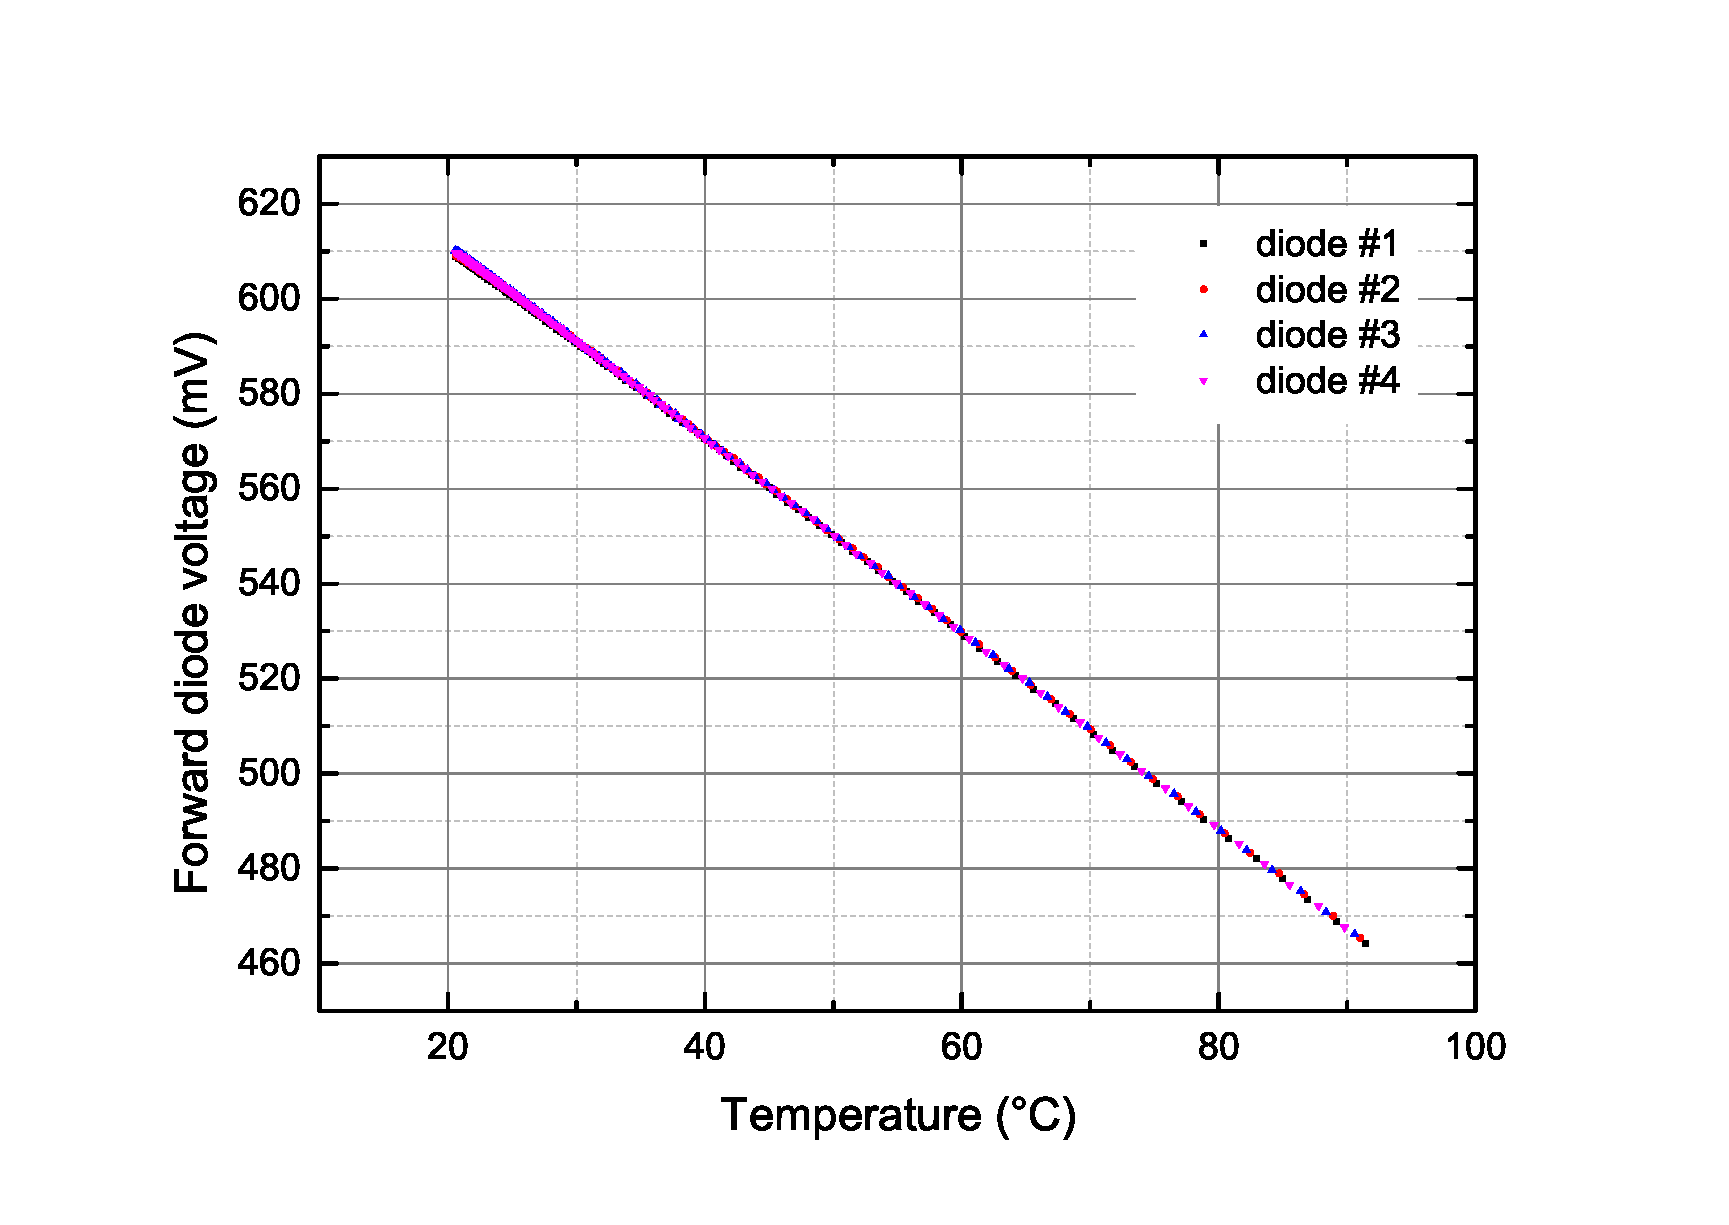
\includegraphics[width=0.7\paperwidth]{img/05/mg_diode_temp.eps}
        \caption{Body diode temperature calibration. Source: \cite{MGThesis}}
    \end{figure}

\section{Operating point selection}
    A current source value had to be chosen, keeping in mind the requirements and working conditions.

    In theory, a zero-temperature coefficient current would be optimal, but after irradiation it could shift slightly, causing a significant error. Additionally, due to limited availability of elements on the market and slight differences between devices, this operating point would be very difficult to achieve.

    As a tradeoff between low temperature coefficient and low starting threshold voltage, (to increase sensor range) the current value of \SI{125}{\micro\ampere} was chosen.

\chapter{Engineering model}
\label{Engineering_model_chapter}
This chapter will describe engineering model developed during this thesis.

This model should be as close to flight model as possible - but it could be e.g. on separate board, which is this case.

This model was developed as flight-ready version for sensor calibration \& tests along with developing \& testing flight software.

\section{Background - calibration stand}
    During development of the system previous model was developed to test and calibrate MOSFET transistors to use as a radiation dosimeters. Calibration stand was developed by M. Gumiela in his engineering thesis \cite{MGThesis}. The basic goal was to develop measurement device which can be used to determine final operational point, calibrate radiation response and to perform temperature calibration of flight sensor.

    The test and calibration stand allows to carry out simultatenous investigation of parameters of multiple MOSFETs (i.e. 18) and diodes (i.e. 6). It is possible to obtaing transfer characteristics of the DUT (I-V) utilizing adjustable constant current source, thermal calibration (Vth(T), Vd(T)) thanks to precise reference thermometers, Iztc investigation and finally TID on-line calibration.


\section{Block diagram}
    Block diagram of proposed system based on CD4007 is presented in the figure \ref{sensor_block_diagram}.

    It was designed having in mind miniaturization of sensor - to fit on PW-Sat2 PLD board. Because CD4007 has 3 complementary MOS pairs it was proposed to use 3 p-MOS transistors as TID sensors - to improve fidelity of the measurements. One n-MOS is used as a temperature sensor. Current source and ADC are multiplexed between 4 channels - this reduces board footprint and increases sensor reliability \& accuracy. Having in mind readout fidelity 3-wire method on multiplexer was implemented.

    System consists of few basic building blocks, each of them will be detailed in this chapter:
    \begin{itemize}
        \item \SI{125}{\uA} constant current source,
        \item CD4007 sensing element (3x p-MOS \& 1x n-MOS),
        \item differential ADC,
        \item multiplexer
    \end{itemize}


    \begin{figure}[H]
        \centering
        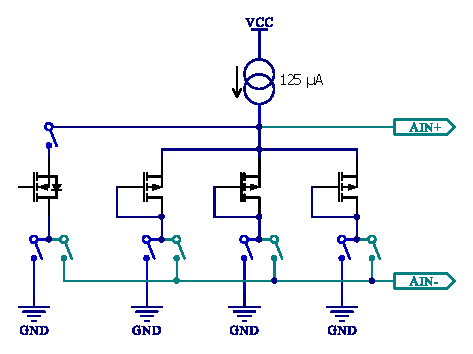
\includegraphics[width=0.7\paperwidth]{img/06/CD4007_mux_schematic.eps}
        \caption{Block diagram}
        \label{sensor_block_diagram}
    \end{figure}

\section{Low-level requirements}
    Using design requirements \ref{Design_requirements} and characteristic curves from \ref{Characteristic_curves} low-level specifications were listed:
    \begin{itemize}
        \item operating temperature range: $0 \div 60 \si{\degreeCelsius}$,
        \item compensated threshold voltage stability: \SI{\pm 0.5}{\milli\volt},
        \item current source value: $\SI{125}{\micro\ampere} \pm \SI{50}{\nano\ampere}$,
        \item ADC resolution: \SI{0.1}{\milli\volt} @ \SI{5}{\volt} reference = \SI{16}{bit}
    \end{itemize}


\section{Analog front-end}
    In this section decision and schematic diagrams of building blocks are presented.

    \subsection{SPICE models}
        Design should be validated by simulation. In this thesis, LTSpice XVII was used.

        Models used during simulation:
        \begin{itemize}
            \item CD4007 - model RIT4007P7 from Rochester Institute of Technology \cite{RIT_FULLER},
            \item Linear Technology components are embedded in LTSpice,
            \item other devices were modelled by hand using datasheets
        \end{itemize}

    \subsection{Linear regulator}
        Positive rail $+\SI{5}{V}$ on PC-104 stack comes from EPS, more specifically, this voltage is generated by DC-DC converter (with \SI{500}{\kilo\hertz} switching frequency). Because of low noise requirements analog supply voltage have to be very well regulated and filtered. Because $V_{TH}$ of transistor will increase with absorbed dose, dropout from \SI{5}{\volt} should be as low as possible. As a tradeoff between this requirement and available solutions on market analog rail voltage was chosen to be \SI{4.7}{\volt}.

        As an LDO regulator LT3042 was selected. It is ultralow noise, ultrahigh PSRR RF linear regulator by Linear Technology. Key specs \cite{LT3042_datasheet}:
        \begin{itemize}
            \item ultralow noise \SI{0.8}{\micro\volt RMS} (\SI{10}{\hertz} to \SI{100}{\kilo\hertz}),
            \item output current \SI{200}{\milli\ampere}
            \item input range \SI{1.8}{\volt} to \SI{20}{\volt}, output range \SI{0}{\volt} to \SI{15}{\volt}
            \item ultrahigh PSRR \SI{79}{\decibel} at \SI{500}{\kilo\hertz}, more detailed graph is shown in the figure \ref{LT3042_PSRR}.
            \item low dropout voltage of \SI{200}{\mV}
        \end{itemize}

        \begin{figure}[H]
            \centering
            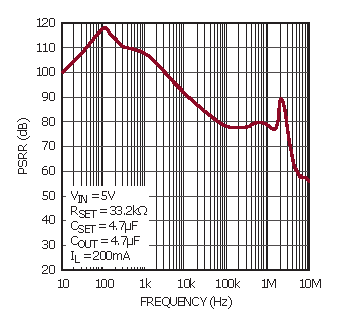
\includegraphics[width=0.4\paperwidth]{img/06/LT3042_PSRR.eps}
            \caption{LT3042 PSRR. Source: \cite{LT3042_datasheet}}
            \label{LT3042_PSRR}
        \end{figure}

        Thanks to this regulator, conducted susceptibility requirement was met (\SI{175}{\mV} input ripple is cut down to \SI{19}{\uV}, which is enough for ADC to filter).

    \subsection{RadFET power switch}
        Because main PLD microcontroller is also controlling other sensors (photodiodes, temperature sensors) RadFET analog front-end have to have a possibility to be turned off. For this purpose, TPS2551DBVx current-limited power-distribution switch was implemented in the design.

        More accurately, two of them - one to disable digital part of ADC and second to disable all analog part of the design.

        Apart from possibility of disabling RadFET they provide point-of-load latch-up current limitation, allowing to cut down power in case of SEE even faster.

    \subsection{Current source}
        Current source have to be the most accurate part of the design, because measured voltage depends in square of its variation. It was assumed that $\SI{50}{\nano\ampere}$ current stability across temperature and aging range will be sufficient. Current source have to supply both MOSFET (static resistance in operating point of about $20-25$~\si{\kilo\ohm}) and body diode temperature sensor (static resistance in operating point of about     $3-7$~\si{\kilo\ohm})

        Main concept of current source is based on Burr-Brown application note \cite{Make_a_precision_current_source_or_sink}. Idea schematic is shown in the figure \ref{current_source_schematic}.

        \begin{figure}[H]
            \centering
            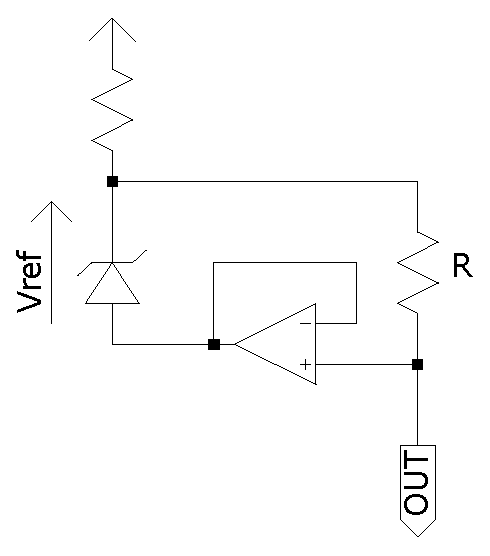
\includegraphics[width=0.3\paperwidth]{img/06/current_source_schematic.eps}
            \caption{Threshold voltage readout block diagram}
            \label{current_source_schematic}
        \end{figure}

        Output current is set by shunt voltage reference and resistor $R$, given by equation:
        $$I_{OUT} = V_{ref}/R$$

        Therefore, stability of output current depends on reference voltage and resistor accuracy.

        \bigskip \textbf{Shunt reference}

        After irradiation MOSFET $V_{DS}$ is planned to be no more than \SI{2.5}{\volt}, so reference voltage have to be lower than \SI{2}{\volt}.

        Linear Technology LT1634-1.25 shunt voltage reference was chosen. It is one of the best shunt references from Linear Technology. Basic specification:
        \begin{itemize}
            \item \SI{0.05}{\percent} initial accuracy,
            \item \SI{10}{ppm/\degreeCelsius} maximum temperature drift,
            \item $< \SI{1}{\ohm}$ dynamic resistance,
            \item \SI{10}{\uA} minimal regulation current
        \end{itemize}

        Shunt resistance was chosen to make minimal current flowing through shunt reference large enough for specified loads - final value of \SI{5}{\kilo\ohm}.

        \bigskip \textbf{Series resistor}

        Value of this resistor reflects required current flowing through MOSFET. Nominal value selected was \SI{10}{\kilo\ohm}.

        Stability of this resistor across temperature is critical because it directly changes output current. To achieve specified requirement \SI{10}{\kilo\ohm} / \SI{5}{ppm} resistor was chosen (APC0603T10K0Z).

        Manufacturer does not specify exact value and profile of the temperature coefficient - so both worst cases was simulated (\SI{-5}{ppm} and \SI{5}{ppm}).

        \bigskip \textbf{Operational amplifier}

        Operational amplifier in this circuit should have very low bandwidth (noise limitation), low offset voltage (precision) and small footprint. LTC2054 was selected - key characteristics:
        \begin{itemize}
            \item \SI{3}{\micro\volt} offset voltage,
            \item common mode $\pm \SI{0.5}{\volt}$ input/output range,
            \item \SI{500}{\kilo\hertz} gain-bandwidth product,
            \item device in Military Plastic package (temperature range $-55 \div \SI{150}{\degreeCelsius}$)
        \end{itemize}

        \bigskip \textbf{Simulation}
        Behavioral simulations were performed to found all possible problems with circuit:
        \begin{itemize}
            \item temperature dependency,
            \item output resistance range,
            \item noise and stability
        \end{itemize}

        MOSFET/diode was replaced by resistor emulating its static resistance ($\SI{2}{\volt}/\SI{125}{\micro\ampere} = \SI{16}{\kilo\ohm}$, $\SI{0.6}{\volt}/\SI{125}{\micro\ampere} = \SI{5}{\kilo\ohm}$, respectively). Simulation view is shown in the figure \ref{current_source_simulation}.

        \begin{figure}[H]
            \centering
            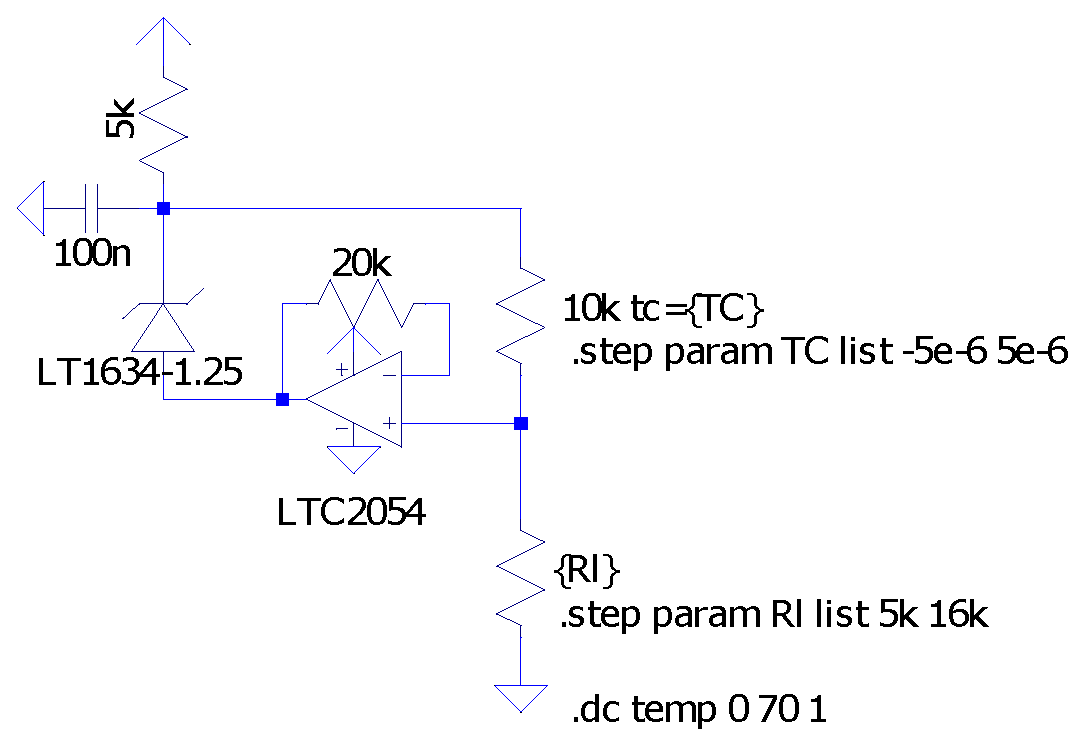
\includegraphics[width=0.5\paperwidth]{img/06/current_source.eps}
            \caption{Current source simulation}
            \label{current_source_simulation}
        \end{figure}

        \bigskip\textbf{Temperature dependency}
        Output current is shown in the figure \ref{current_source_simulation_result}, simulation was performed on two different loads and resistor temperature coefficients.
        \begin{figure}[H]
            \centering
            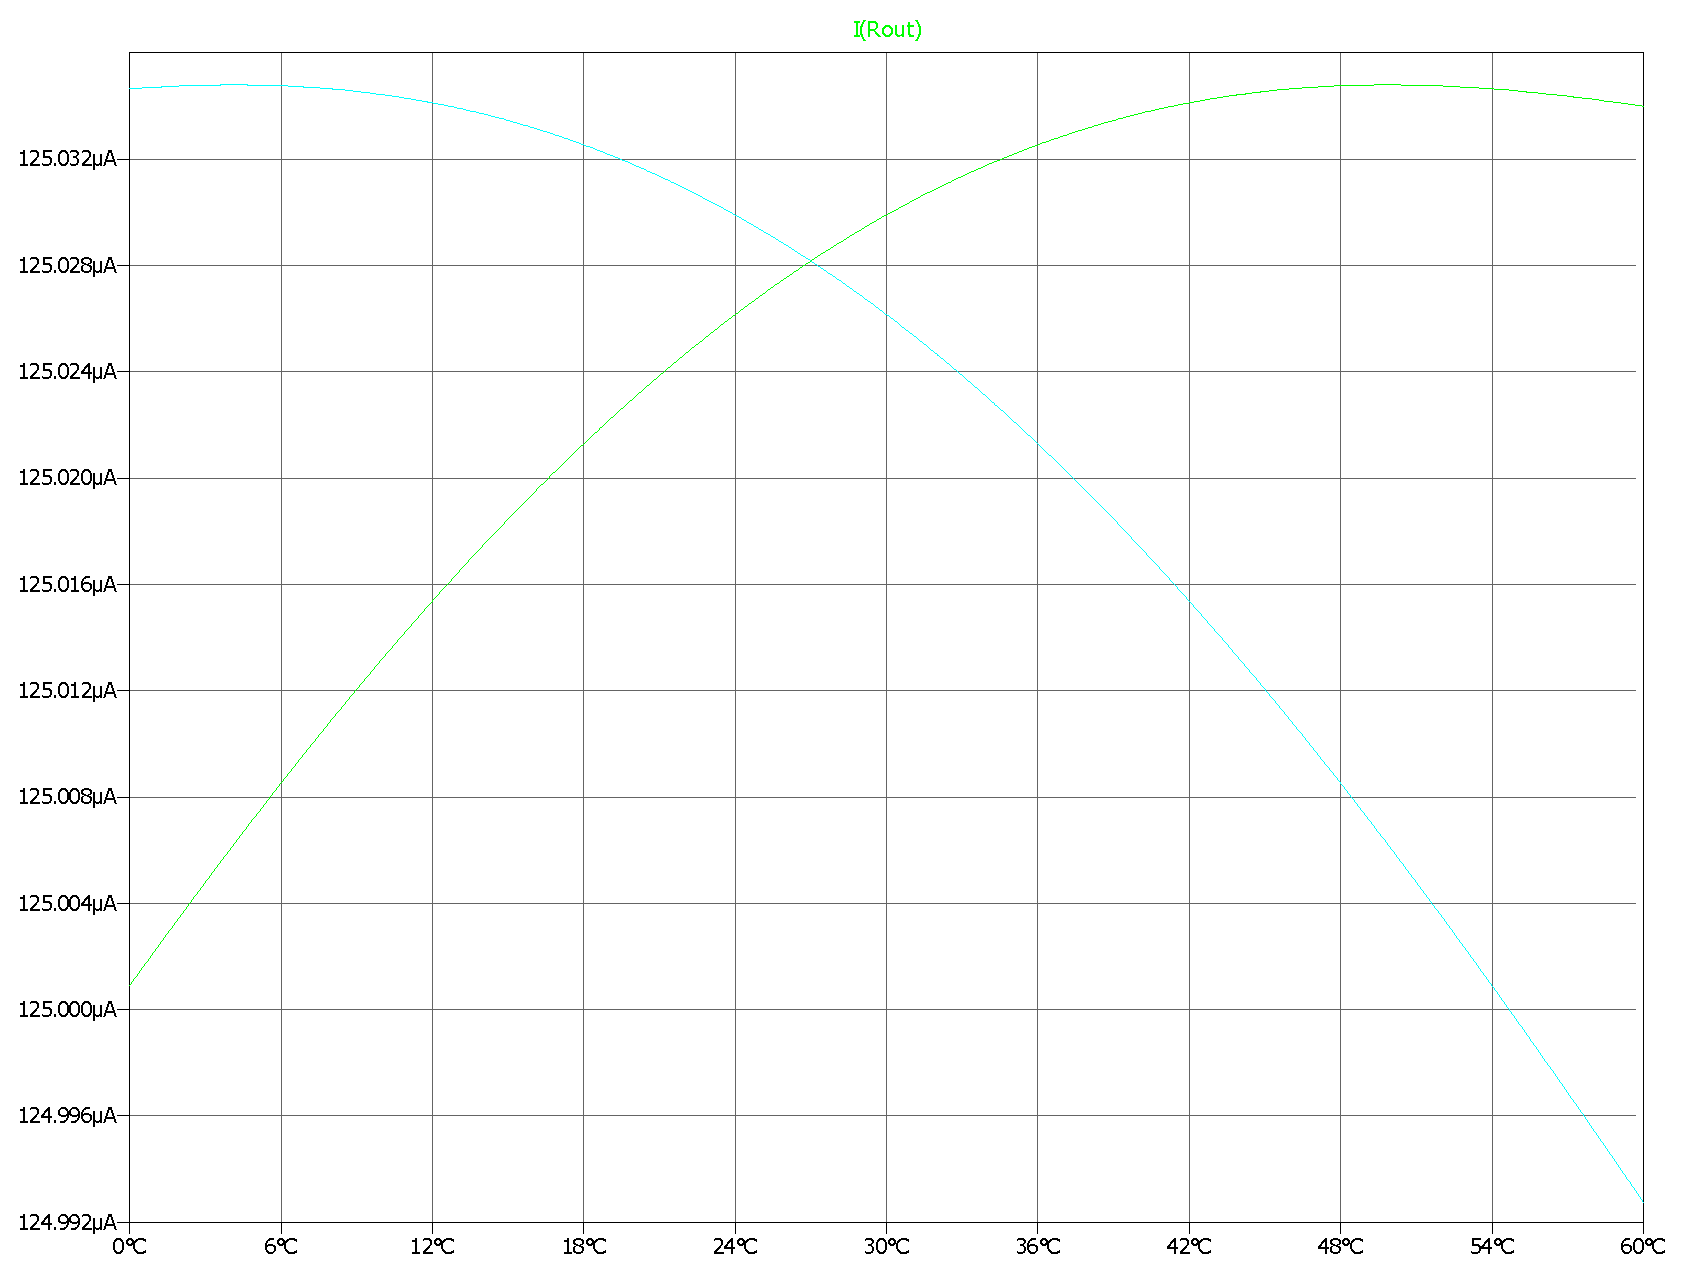
\includegraphics[width=0.8\paperwidth]{img/06/current_source_result.eps}
            \caption{Current source simulation result - output current}
            \label{current_source_simulation_result}
        \end{figure}

        In both cases current change across temperature range does not exceed \SI{40}{\nano\ampere}.

        \bigskip\textbf{Output resistance range}
        \bigskip\textbf{Noise density}
        \bigskip\textbf{Stability}

    \subsection{Analog to digital converter}
        Analog to digital converter is responsible for reading $V_{DS}$ voltage across transistor and voltage across diode. Due to very low changes, high accuracy and resolution is required. Additionally, complex mixed signal element like ADC should have radiation tests to prove its long term reliability. To achieve at least \SI{0.1}{\milli\volt} resolution ADC has to be at least \SI{16}{bits}.

        Due to constrain on system and reliability the AD7714 from Analog Devices was chosen. Radiation tests shown that it fails between \SI{10}{\kilo\rad} and \SI{20}{\kilo\rad}, with no degradation up to \SI{10}{\kilo\rad} \cite{ADC_radiation_tests}.

        Internal diagram can be found in the figure \ref{AD7714}. Key specs:
        \begin{itemize}
            \item \SI{24}{bits},
            \item \SI{0.0015}{\percent} nonlinearity,
            \item programmable gain ($1 \div 128$),
            \item 3 fully differential or 5 pseudo-differential input channels
            \item \SI{3}{\volt} or \SI{5}{\volt} operation
            \item separated digital and analog supply and grounds,
            \item SPI interface
            \item \SI{0.25}{\hertz} sampling frequency for strongest filter,
        \end{itemize}

        \begin{figure}[H]
            \centering
            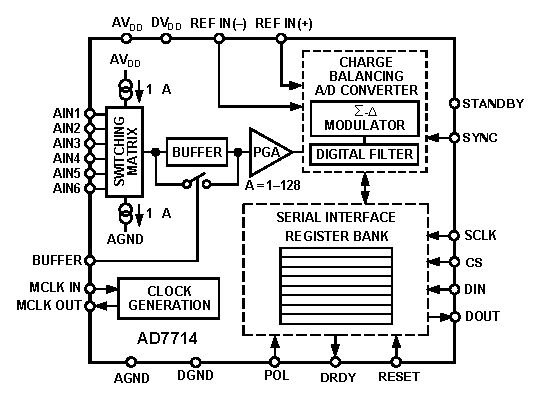
\includegraphics[width=0.5\paperwidth]{img/06/AD7714.eps}
            \caption{AD7714 internal block diagram. Source: \cite{AD7714_datasheet}}
            \label{AD7714}
        \end{figure}

        AD7714 requires external crystal or clock oscillator in frequency range \SI{1}{\mega\hertz} to \SI{2.54}{\mega\hertz}. Crystal oscillators for these frequencies are large and susceptible for shocks and damages because of large, delicate internal structure. \SI{1}{\mega\hertz} ceramic oscillator ISM95-3351AH was selected for operation. Comparison of solution in shown in the figure \ref{crystal_oscillator_difference}.

        \begin{figure}[H]
            \centering
            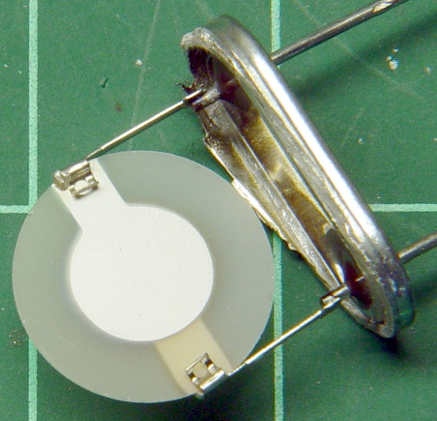
\includegraphics[width=0.35\paperwidth]{img/06/crystal.png}
                        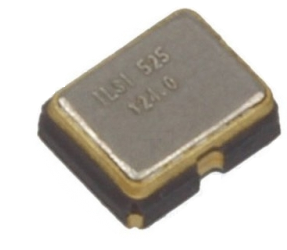
\includegraphics[width=0.35\paperwidth]{img/06/ISM95.png}
            \caption{Low frequency crystal oscillator internals. Source: \cite{Opening_a_Quartz_Crystal_Can_Effects_Thereof}, ISM95-3351AH-1.0000 ceramic oscillator package. Source: \cite{ISM95_series_datasheet}}
            \label{crystal_oscillator_difference}
        \end{figure}

    \subsection{Multiplexer}
        Multiplexer have two purposes: to multiplex current and voltage lines (3-wire readout).

        As an analog multiplexer ADG709 was chosen. Its radiation tests can be found in \cite{IEEE_radiation_tests_1992_2009}. It is double 1:4 mux, allowing simultaneous current and voltage multiplexing. Internal block diagram is shown in the figure \ref{ADG709_block}

        \begin{figure}[H]
            \centering
            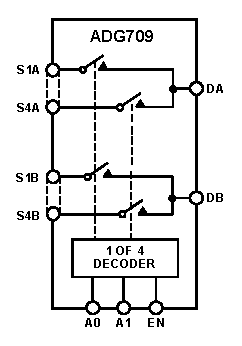
\includegraphics[width=0.3\paperwidth]{img/06/ADG709.eps}
            \caption{ADG709 internal block diagram. Source: \cite{ADG709_datasheet}}
            \label{ADG709_block}
        \end{figure}

        Due to ESD diodes id CD4007 additional current switch had to be added to cut off potential from from n-MOS body diode. For this purpose simple 1-channel analog switch ADG849YKSZ was implemented.

    \subsection{Differential \& common mode filter}
        Internal sampling frequency of ADC (for GAIN = 1 and $f_{clk} = \SI{1}{\mega\hertz})$ is about \SI{15.6}{\kilo\hertz}. To eliminate aliasing and reduce readout noise low-pass differential filter should be implemented on ADC input.

        Simple one-pole RC filter was selected. Its schematic can be found in the figure \ref{low_pass_filter}.

        \begin{figure}[H]
            \centering
            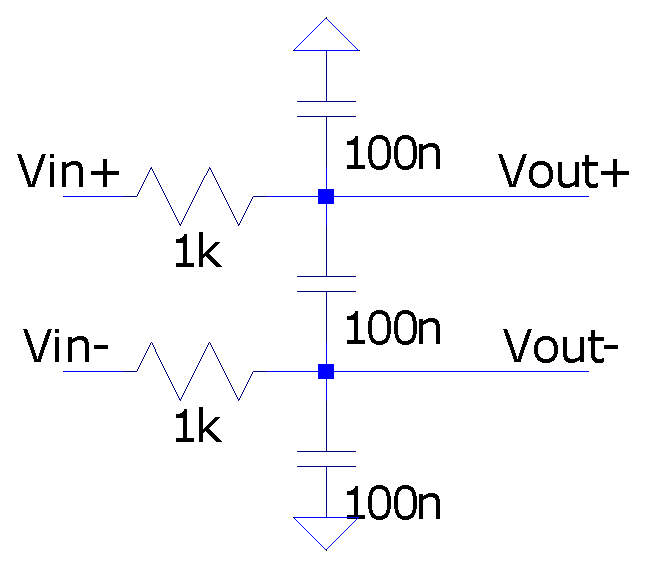
\includegraphics[width=0.3\paperwidth]{img/06/low_pass_filter.eps}
            \caption{Low pass filter schematic.}
            \label{low_pass_filter}
        \end{figure}

        Using AC analysis its frequency characteristic was obtained - figure \ref{low_pass_filter_output}. At half of sampling frequency attenuation is about \SI{22}{\decibel}.

        \begin{figure}[H]
            \centering
            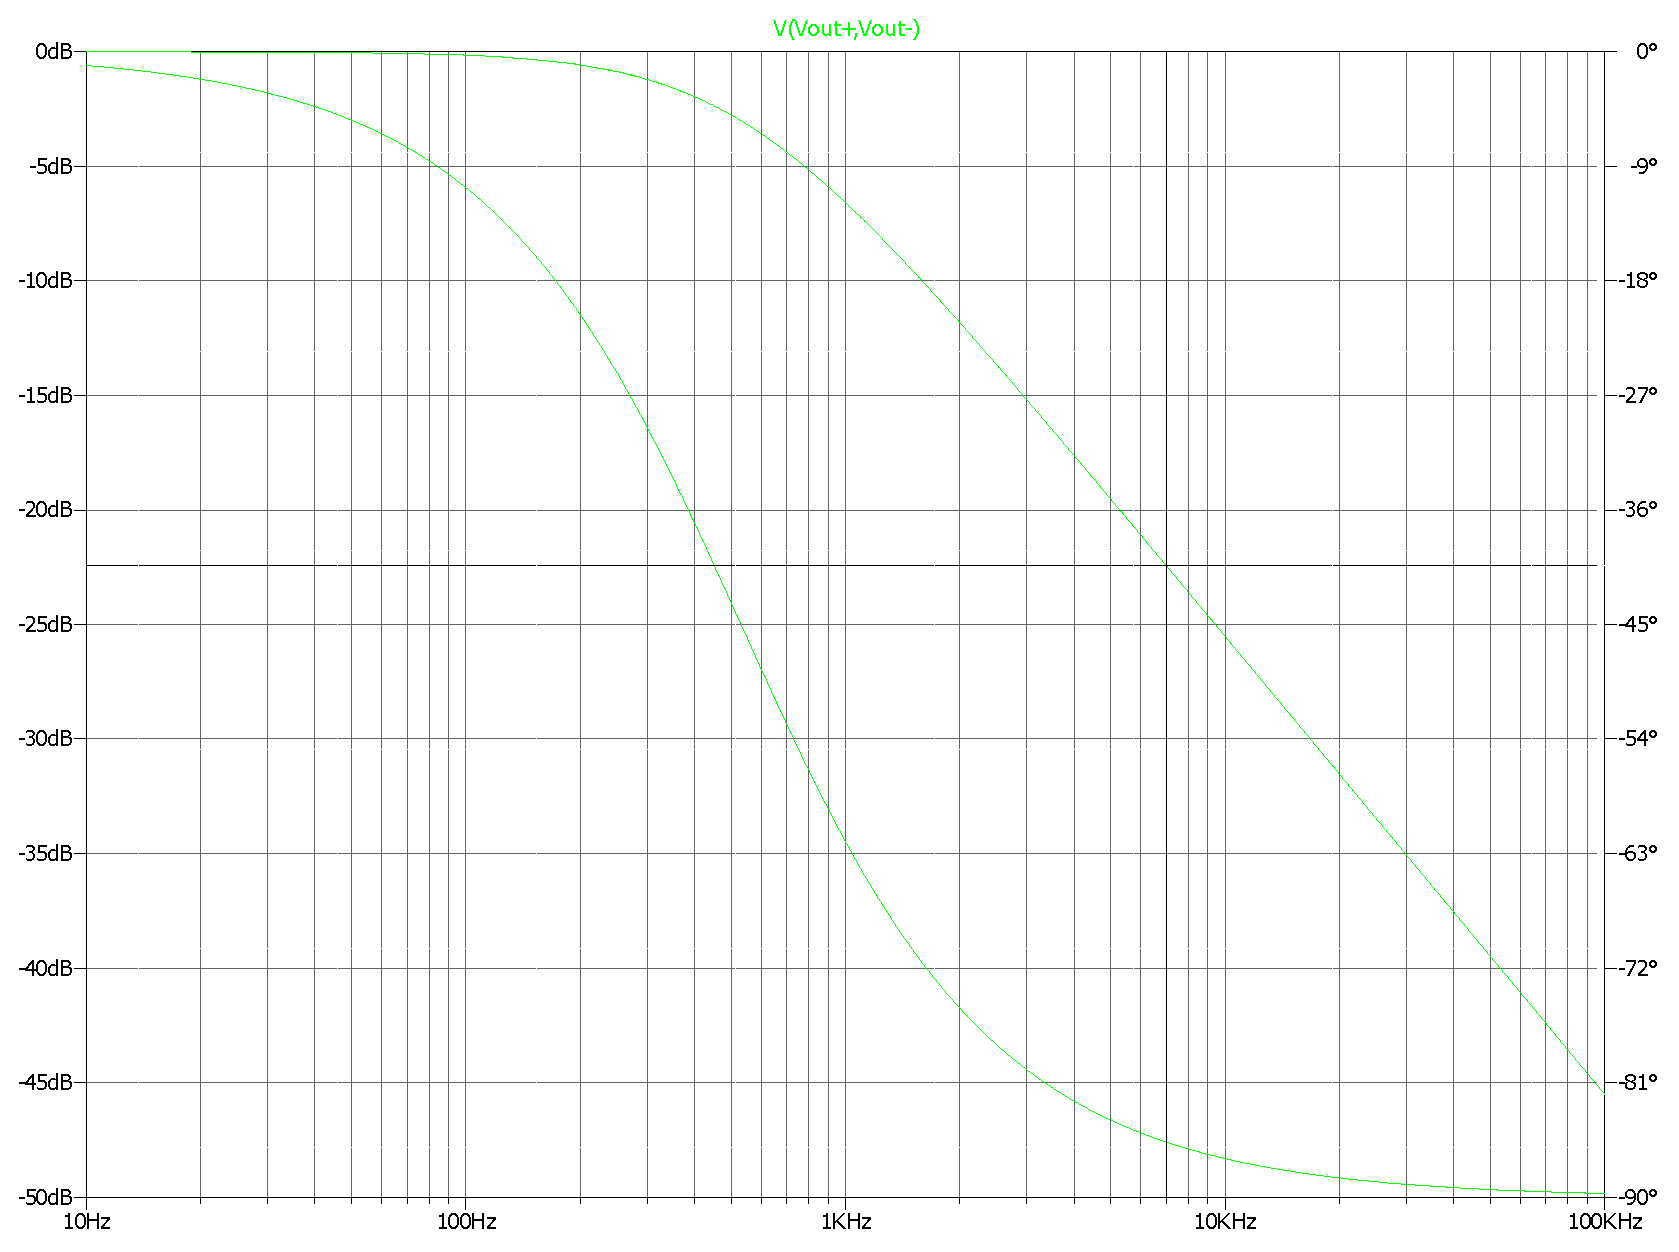
\includegraphics[width=0.6\paperwidth]{img/06/low_pass_filter_output.eps}
            \caption{Low pass filter frequency characteristics.}
            \label{low_pass_filter_output}
        \end{figure}

    \subsection{Shielding}
        Because of noise requirements and near proximity of \SI{0.5}{\watt} radio transmitter, EMI shielding was tested.

        Proper pads for EMI shielding were placed on PCB. Its size depends on PCB layout, after routing it was decided to use BMI-S-203 shield (figure \ref{BMI-S-203}). This shield should provide attenuation of about \SI{50}{\decibel} on transmitter frequency.

        \begin{figure}[H]
            \centering
            
\includegraphics[width=0.7\paperwidth]{img/06/BMI-S-203.eps}
            \caption{BMI-S-203 shield. Source: \cite{EMI_shieldings_catalog}}
            \label{BMI-S-203}
        \end{figure}


\section{Digital}
    RadFET is mainly analog sensor. But, LDO, MUX and ADC has to be controlled from on-board microcontroller. On other hand, RadFET have to be accessible from OBC, to retrieve data and send them to the ground station.

    \subsection{Microcontroller}
        Main digital part of the design is microcontroller. It will be responsible for:
        \begin{itemize}
            \item controlling analog part of the sensor,
            \item implementing FDIR in case of any failure,
            \item communicating with OBC to retrieve data.
        \end{itemize}

        Couple of options were considered, and the final choose was ATmega164PV-10AQ. More detailed comparison can be found in \cite{PWSAT_EPS_CDR}.

        AVR devices are known from their simplicity, reliability and very little bugs. Radiation tests were performed for ATmega series, showing their performance for up to \SI{14}{\kilo\rad} \cite{ATMEGA128_radiation_tests}.

        Features of this particular device:
        \begin{itemize}
            \item \SI{1.8}{\volt} - \SI{5.5}{\volt} supply voltage,
            \item \SI{4}{\mega\hertz} clock,
            \item TQFP-44 package,
            \item \SI{16}{\kilo B} program memory,
            \item \SI{1}{\kilo B} SRAM
        \end{itemize}

    \subsection{On-Board Computer interface}
        Interface to OBC is $I^2C$ bus. Because sensor can be turned off by cutting its voltage proper buffering had to be implemented. For this purpose $I^2C$ repeater PCA9517 was placed between OBC and in-sensor microcontroller. Its functional diagram can be seen in the figure \ref{PCA9517}. From its datasheet: "The SDA and SCL pins are over voltage tolerant and are high-impedance when the PCA9517 is unpowered." \cite{PCA9517_datasheet}. Thanks to it OBC can completely disable the sensor, by simply cutting it a power.

        \begin{figure}[H]
            \centering
            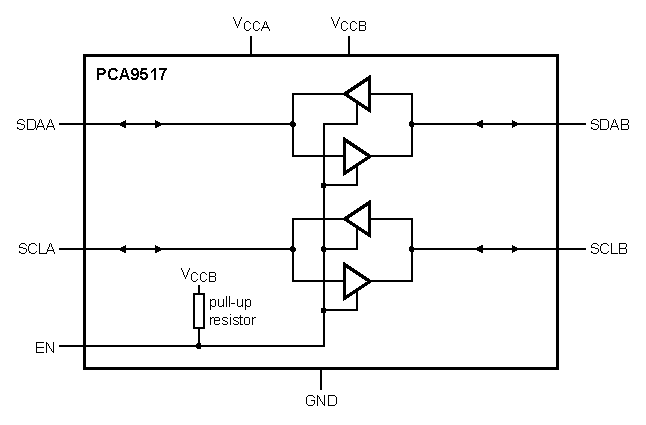
\includegraphics[width=0.7\paperwidth]{img/06/PCA9517.eps}
            \caption{PCA9517 internal block diagram. Source: \cite{PCA9517_datasheet}}
            \label{PCA9517}
        \end{figure}


\section{Final schematic}
    Top level schematic file can be seen in the figure \ref{top_level_schematic}. Ports represents physical connectors - to satellite bus and debug socket.

    \begin{figure}[H]
        \centering
        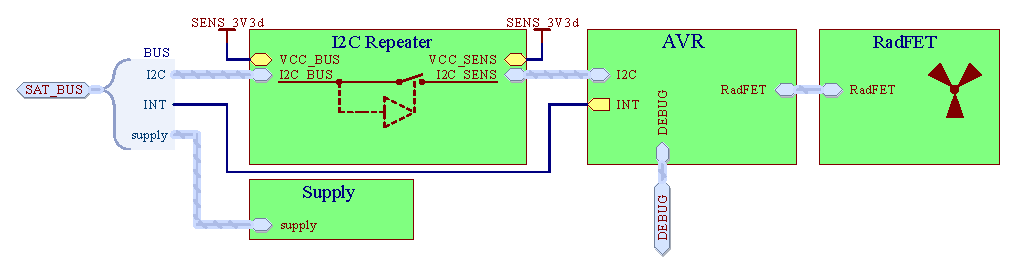
\includegraphics[width=0.8\paperwidth]{img/06/final_schematic_top.eps}
        \caption{Top level schematic}
        \label{top_level_schematic}
    \end{figure}

    "RadFET" consists analog part of the design. Its block diagram can be seen in the figure \ref{analog_schematic}.

    \begin{figure}[H]
        \centering
        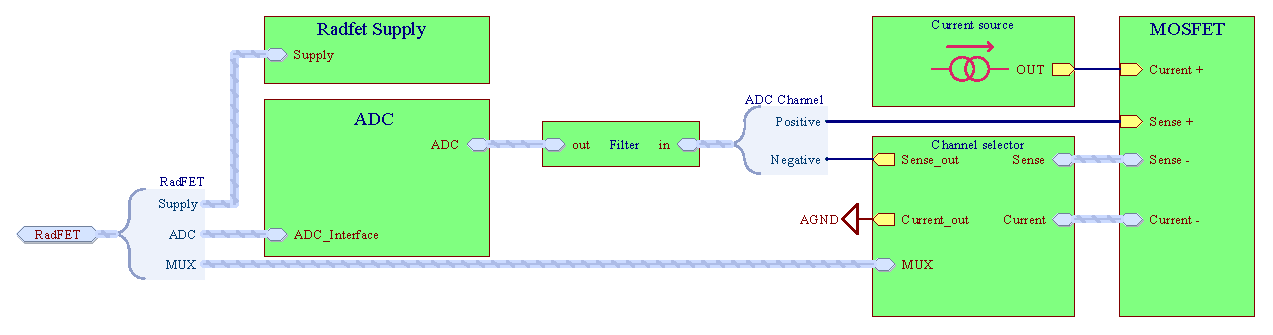
\includegraphics[width=0.8\paperwidth]{img/06/final_schematic_radfet.eps}
        \caption{Sensor final schematic - analog part}
        \label{analog_schematic}
    \end{figure}


\section{PCB}
    Engineering model of the sensor was manufactured on similar board to the flight model. It should represent space required for this sensor, noise coupling and performance.

    For schematic capture, PCB layout \& DRC Altium Designer EDA software was used.

    \subsection{PCB materials}
        During initial phase of PW-Sat2 project it was decided that all self-made board will be manufactured on FR4 laminate. Despite most space-qualified PCBs are made of polimide, it will be very hard (and expensive) to manufacture them. Despite higher glass transition temperature they do not provide much advantages.

        But, careful should be taken to check for:
        \begin{itemize}
            \item vibration tolerance,
            \item gluing quality of multiple layer boards,
            \item outgassing coefficient.
        \end{itemize}

        Having this in mind manufacturer of PCB was selected - Technoservice S.A.

    \subsection{PCB stack}
        Because outgassing of devices can be dangerous for turbomolecular pumps, it have to be limited as much as possible. Therefore soldermask and overlay layers are not present in the design, and packages of used components have known outgassing coefficients.

        For this prototype board have 4 layers, on flight model board will be 6-layered. PCB stack generated from Altium Designer is shown in the figure \ref{PCB_Altium_stack}.

        \begin{figure}[H]
            \centering
            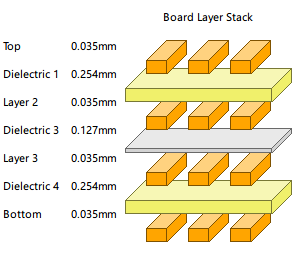
\includegraphics[width=0.3\paperwidth]{img/06/stack.png}
            \caption{Sensor PCB stack}
            \label{PCB_Altium_stack}
        \end{figure}

    \subsection{PCB layout}
        PCB layout in mixed signal board is very important. Ground potential shifts, induced noise, coupling between ground planes - all those effects were considered during layout process.

        \bigskip \textbf{Top \& bottom layers}

        On top and bottom layers only components should be placed, every net should be connected on internal layers. But, because of having only 4-layer board this design recommendation is not fulfilled - this will be forced on Flight Model. Final layout is shown in the figure \ref{top_bottom_layer_layout}.

        \begin{figure}[H]
            \centering
            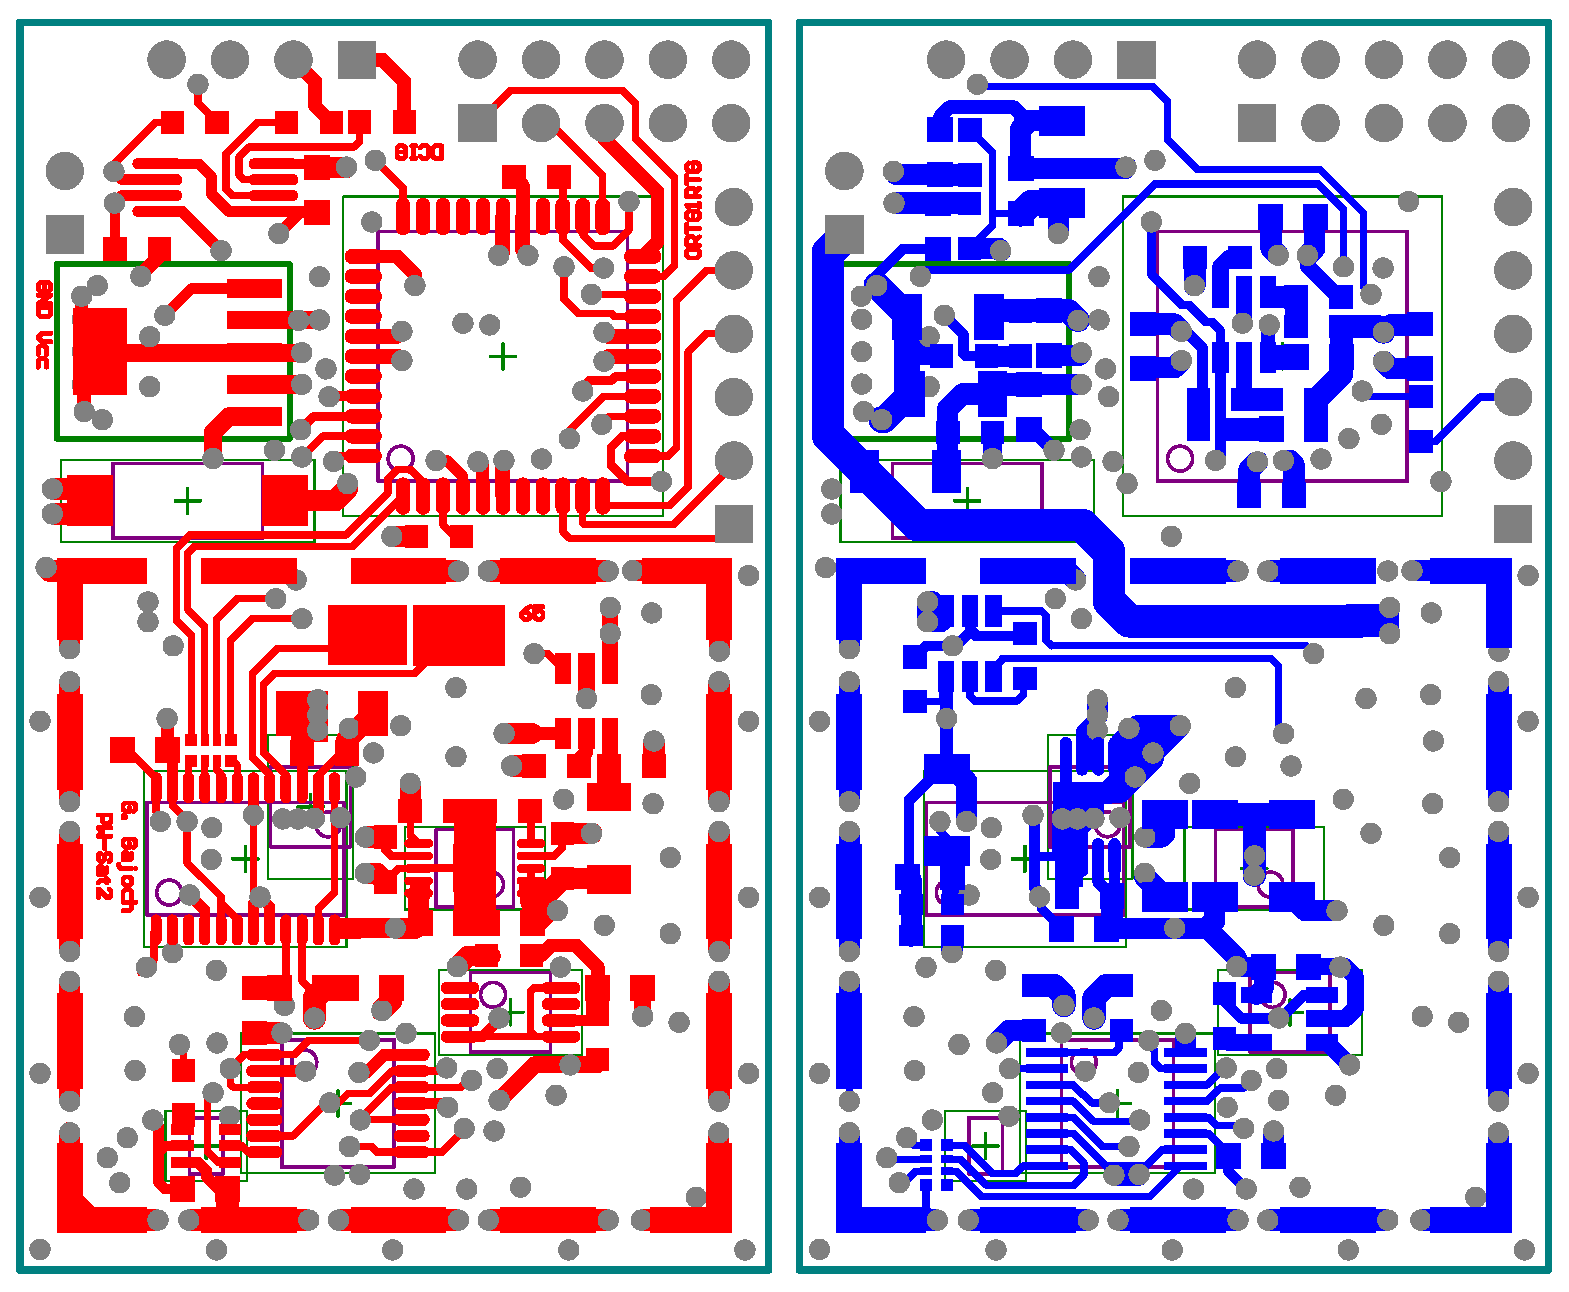
\includegraphics[width=0.5\paperwidth]{img/06/top_bottom_layer_layout.eps}
            \caption{Top and bottom layer layout}
            \label{top_bottom_layer_layout}
        \end{figure}

        \bigskip \textbf{Internal layers}

        One layer of board was designed to be completely a ground plane. More specifically, two ground planes - analog and digital one, connected under ADC. Second internal layer provides routing space, but also have ground planes on it (due to PCB temperature bending PCB cannot have only one ground plane). Layout is shown in the figure \ref{internal_layers_layout}.

        \begin{figure}[H]
            \centering
            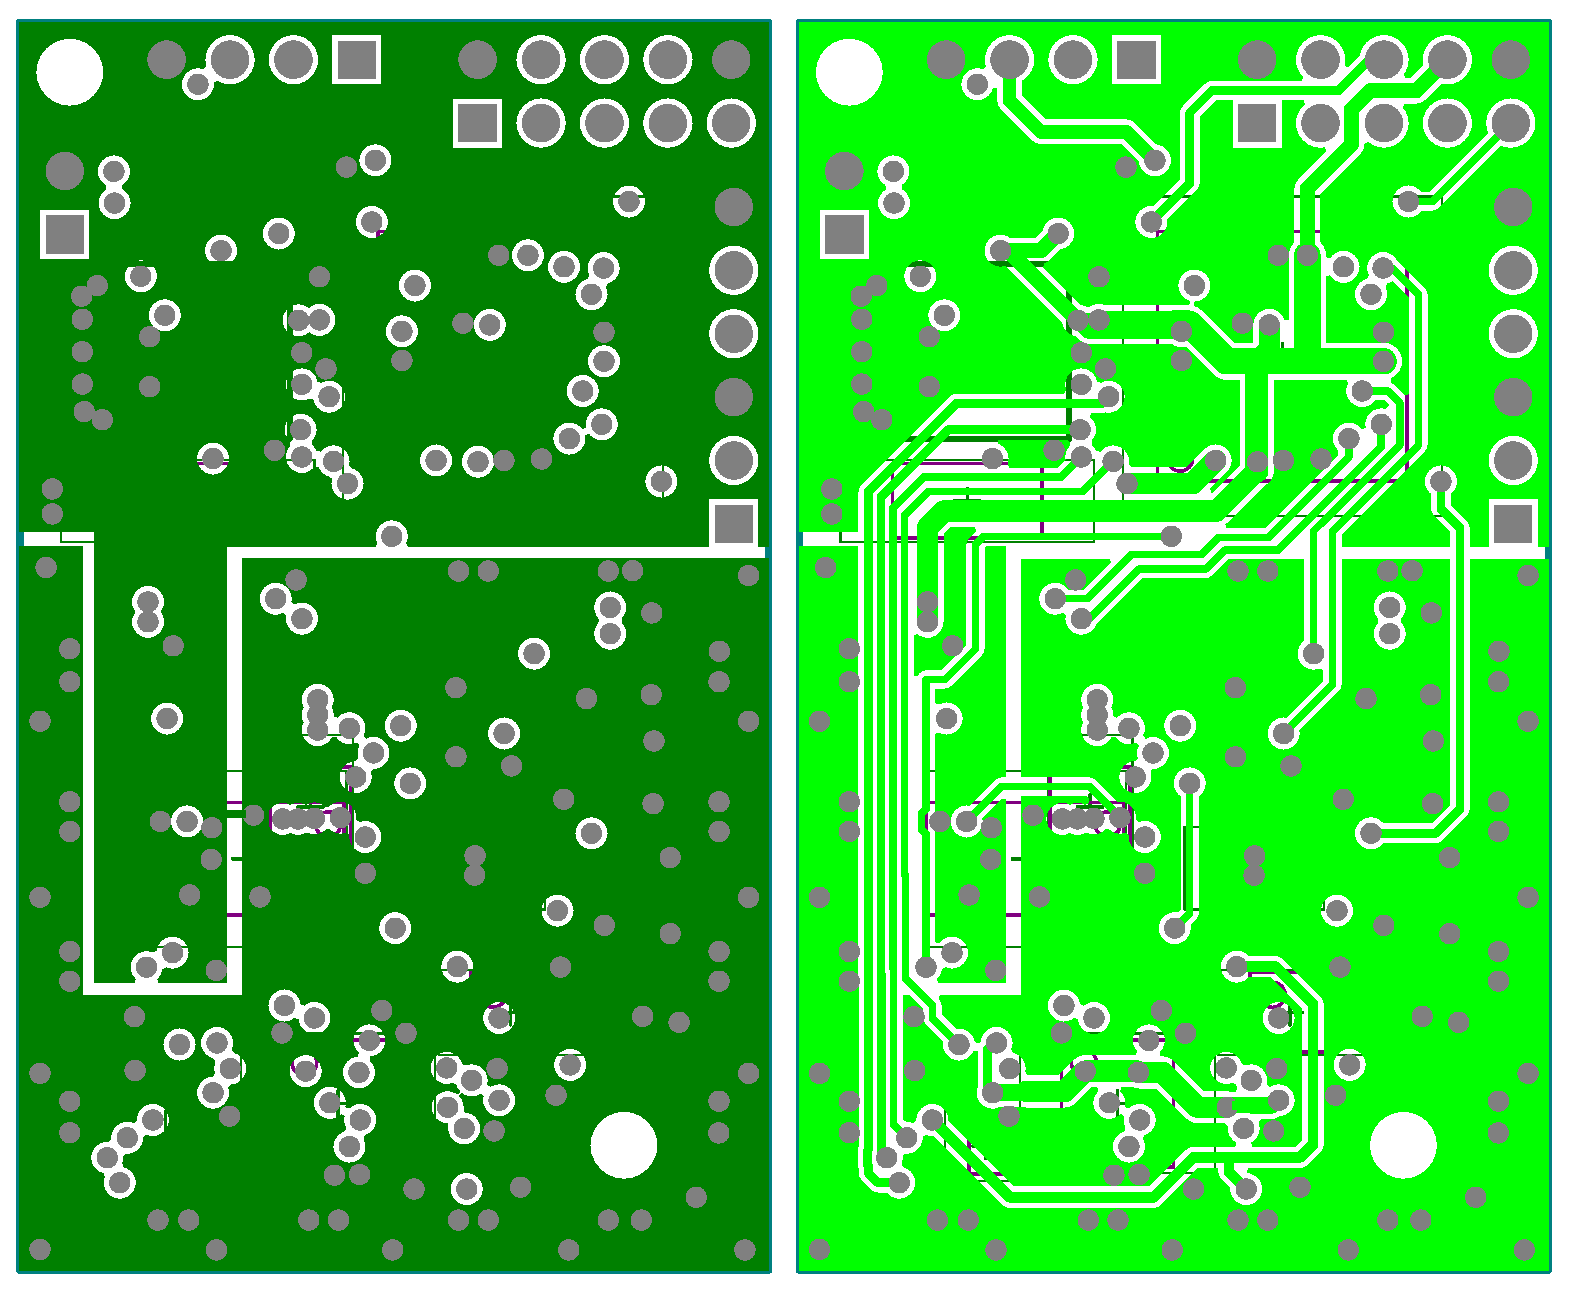
\includegraphics[width=0.5\paperwidth]{img/06/internal_layers_layout.eps}
            \caption{Internal layers layout}
            \label{internal_layers_layout}
        \end{figure}

    \subsection{3D model}
        Using Altium designer and proper self-made libraries, 3D model of board can be easily generated. In the figure \ref{pcb_3d_model} 3D model with and without EMI shielding is shown.

        \begin{figure}[H]
            \centering
            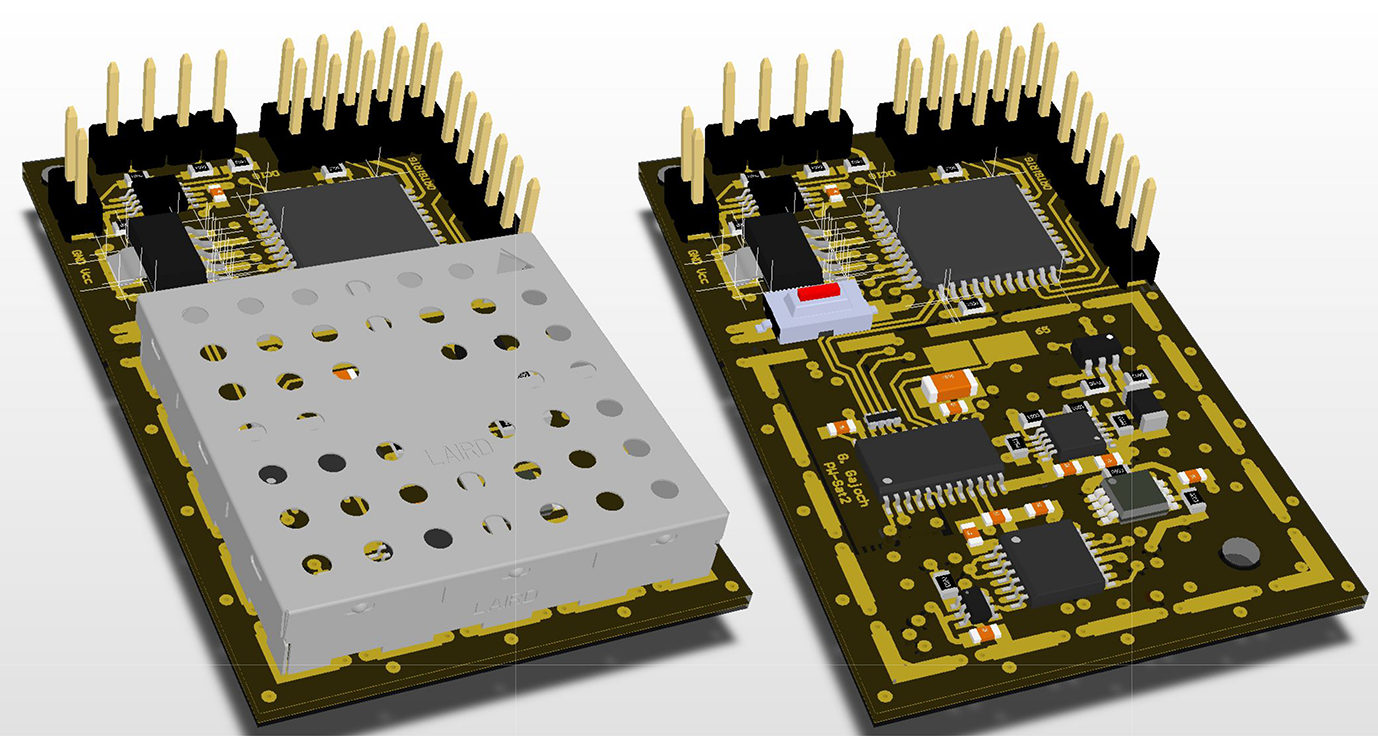
\includegraphics[width=0.8\paperwidth]{img/06/pcb_3d_model.png}
            \caption{3D view of engineering model with and without EMI shield}
            \label{pcb_3d_model}
        \end{figure}

\section{Software design}
    Important aspect of the sensor is embedded software. It has to control data acquisition (LDO, ADC, MUX), check for validity and expose \iic interface to OBC.

    Because main microcontroller is 8-bit AVR-core processor, software have to be highly optimized, especially for speed and data memory consumption. Available resources:
    \begin{itemize}
        \item \SI{16}{\kilo B} of FLASH,
        \item \SI{1}{\kilo B} of SRAM,
        \item \SI{1}{\mega\hertz} clock frequency.
    \end{itemize}

    Software for sensor was written in C++14, using developed by PW-Sat2 team AVR-HAL library. Schematic of software building blocks is shown in the figure \ref{Sensor_software_diagram}.

    \begin{figure}[H]
        \centering
        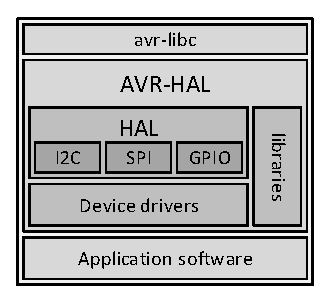
\includegraphics[width=0.5\paperwidth]{img/06/software_diagram.eps}
        \caption{Sensor software diagram}
        \label{Sensor_software_diagram}
    \end{figure}

    \subsection{AVR-HAL}
    AVR-HAL is a library created to ease software development on AVR microcontrollers. It was created by PW-Sat2 team, having in mind low overhead (in most modules zero-data usage), extensibility and modern software development languages and techniques (C++14, unit and integration testing). It was created for specific purpose which is embedded software development on-board PW-Sat modules (EPS, PLD, SunS). Therefore only few devices are officially supported (ATmega164, 165, 328), with extensible tests on existing platforms.

    AVR-HAL consists of basic modules:
    \begin{itemize}
        \item C++14 libraries not existing in avr-libc (type traits, array, array\_view),
        \item Hardware Abstraction Layer - identical low-level API for every ported device,
        \item Device Drivers - drivers for many used integrated circuits used on PW-Sat2,
        \item Debugging libraries - software created to allow unified debugging of many devices (serial port, command line interface, gdb connection etc).
    \end{itemize}

    Using AVR-HAL writing application software is only high-level work, leaving all hardware access to tested and proven library.

    \subsection{$I^2C$-slave interface}
    Cubesat standard define two \iic lines along satellite board stack, which most of the commercially available devices use. It was the easiest option for connecting PLD board to OBC, so this communication bus was selected.

    The sensor acts as a slave on \iic bus. Communication protocol is based on request-reply manner, with interrupt pin acting as a notification.

    When OBC wants to gather data from sensor it will do following tasks in order:
    \begin{itemize}
        \item send measurement start request to sensor (table \ref{Start_measurement_command}),
        \item wait until conversion is completed (pulse on interrupt line is triggered),
        \item read data from sensor internal memory (table \ref{Data_readout_command}).
    \end{itemize}

    \begin{table}[H]
        \begin{center}
            \begin{tabular}{|c|c|c|c|}
                \hline
                START & 0x20+W & 0x80 & STOP \\ \hline
            \end{tabular}
        \end{center}
        \caption{Start measurement command}
        \label{Start_measurement_command}
    \end{table}

    \begin{table}[H]
        \begin{center}
            \begin{tabular}{|c|c|c|c|c|c|c|}
                \hline
                START & 0x20+W & 0x00 & REP-START & 0x20+R & (...data...) & STOP \\ \hline
            \end{tabular}
        \end{center}
        \caption{Data readout command}
        \label{Data_readout_command}
    \end{table}

    \subsection{Measurement algorithm}
    \bigskip \textbf{RadFET sensor}

    Sensor after receiving "start measurement" command (table \ref{Start_measurement_command}) does following steps:
    \begin{itemize}
        \item enable LDO,
        \item wait for power line stabilization,
        \item for each channel in [MOS0, MOS1, MOS2, TEMPERATURE]:
        \begin{itemize}
            \item[$\circ$] select proper MUX switch,
            \item[$\circ$] enable MUX,
            \item[$\circ$] wait for stabilization,
            \item[$\circ$] read ADC value,
            \item[$\circ$] disable MUX
        \end{itemize}
        \item disable LDO,
        \item make a positive pulse on interrupt line, informing OBC about conversion finish.
    \end{itemize}

    \bigskip \textbf{OBC}

    When OBC wants to read data form sensor (issued by telecommand from ground station) it perform following steps:
    \begin{itemize}
        \item enable PLD power by sending proper command to EPS,
        \item send "start measurement" command to RadFET,
        \item wait for trigger on interrupt line (external interrupt pin),
        \item send "data readout" command and store data in memory,
        \item disable power for PLD board
    \end{itemize}

\section{Assembly}
    For final model, proper ECSS standards will be applied during soldering and integration. On engineering model proper tools and techniques should be tested to eliminate unnecessary problems later on.

    Equipment used during soldering and integration are compliant with ECSS standards, same tools would be used on flight hardware:
    \begin{itemize}
        \item Weller WMRP station,
        \item \SI{63}{\percent} Sn/\SI{37}{\percent} Pb \SI{0.2}{\milli\meter} soldering wire,
        \item Alpha RMA - ROL0 flux,
        \item ESD-protected workstation and tools.
    \end{itemize}

\section{Finished sensor}
    Photo of sensor after integration can be seen in the figure \ref{Integrated_sensor}.

    \begin{figure}[H]
        \centering
        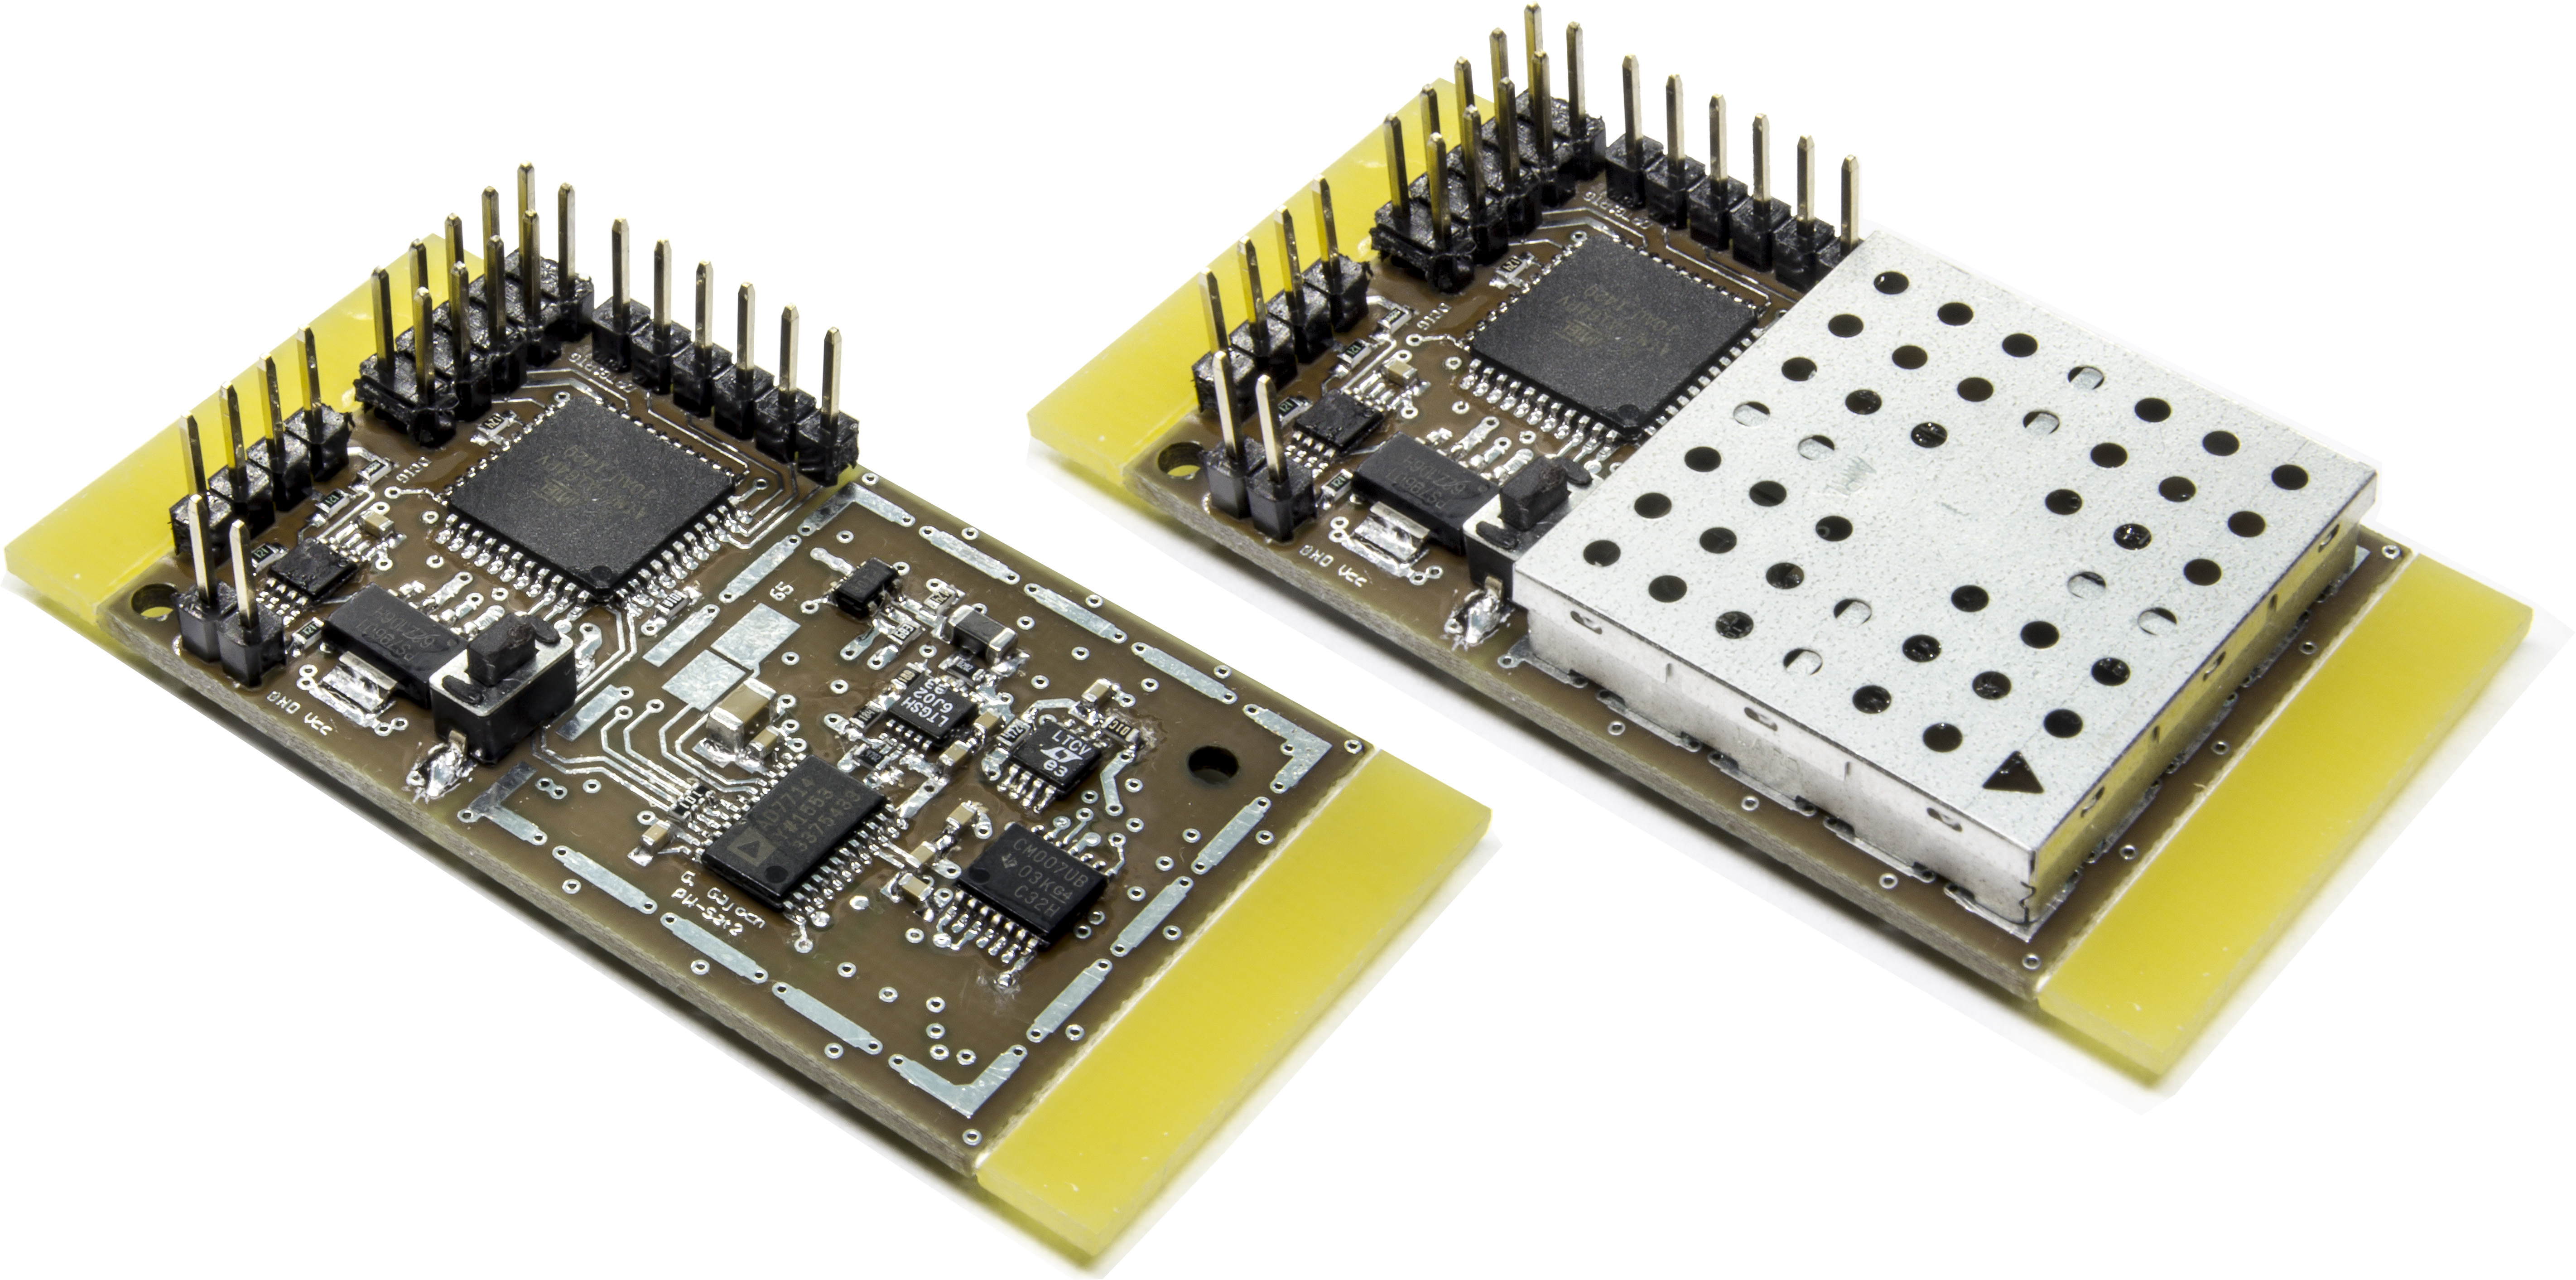
\includegraphics[width=0.8\paperwidth]{img/06/finishiedSensorPhoto.jpg}
        \caption{Integrated sensor without and with EMI shield}
        \label{Integrated_sensor}
    \end{figure}

\chapter{Sensor tests}

%\section{Digital}
%    \subsection{Interface tests}
%    \subsection{Software tests}

\section{Power}
    \subsection{LDO stabilisation}
        Voltage after LDO was measured against time, to calculate the delay between power enablement and measurement start. The time-domain graph is shown in figure \ref{LDO_rise_time}. Delay was estimated to be around \SI{1}{\second}.

        \begin{figure}[H]
            \centering
            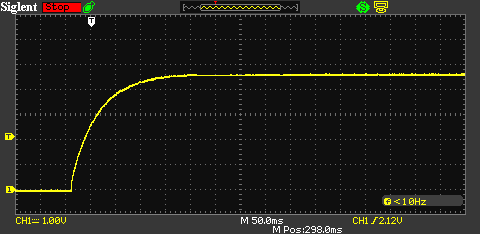
\includegraphics[width=0.8\paperwidth]{img/07/rise_time.png}
            \caption{LDO rise time}
            \label{LDO_rise_time}
        \end{figure}

    \subsection{Power consumption}
        The current drawn during readout is about \SI{25}{\milli\ampere} at \SI{5}{\volt} rail, so the power consumption of the sensor equals \SI{0.125}{\watt}.

\section{Current source}
    Current source was tested on HP 34970A - 6 1/2 digit multimeter, with 200 power line cycle integration enabled.

    \subsection{Noise}
        The noise of the current source was measured for a long period of time, taking a sufficient number of samples. The results (\ref{Current_Stability}) show that the noise floor is below specification for this meter.

        \begin{figure}[H]
            \centering
            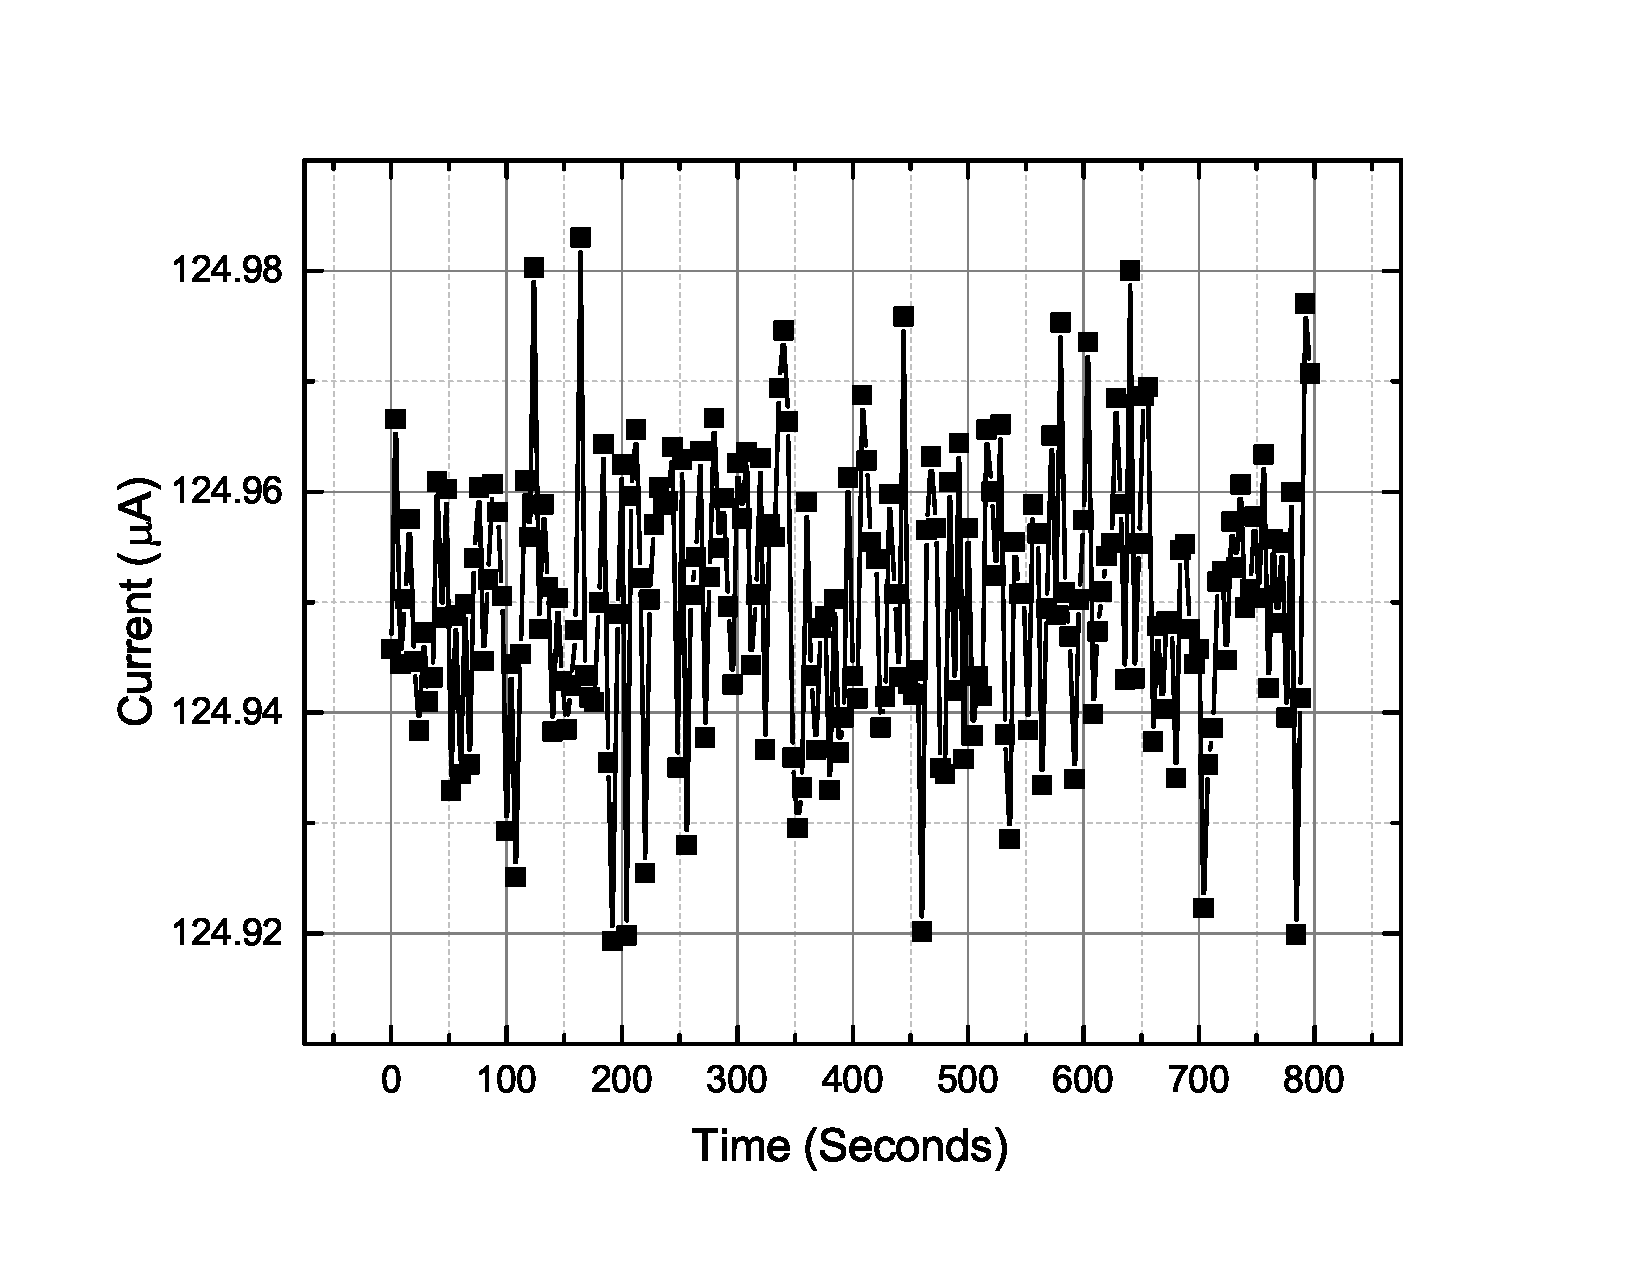
\includegraphics[width=0.6\paperwidth]{img/07/current_time.eps}
            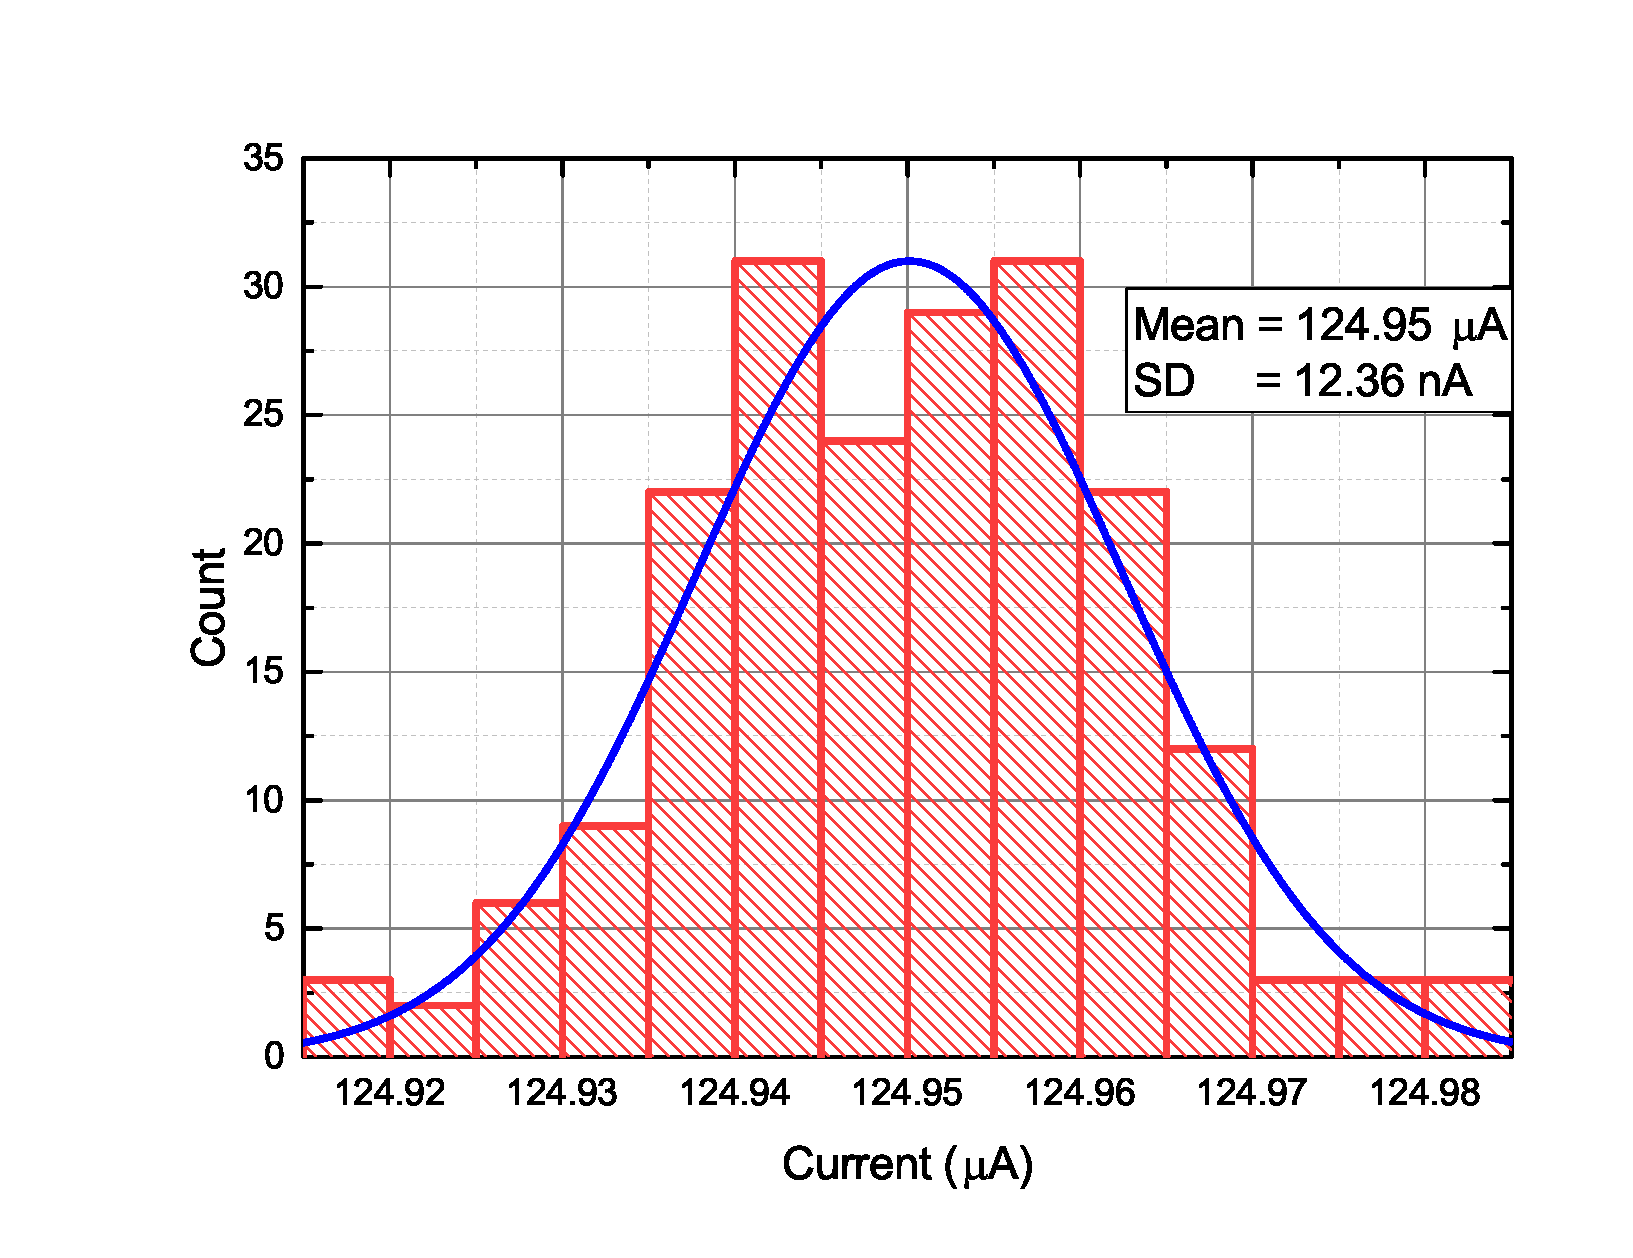
\includegraphics[width=0.6\paperwidth]{img/07/current_hist.eps}
            \caption{LDO rise time}
            \label{Current_Stability}
        \end{figure}

    \subsection{Load range}
        Output load was changed identically as it was in simulation, to test its fidelity. Simulation and build models show the same range and stability - confirming the design. The current source works as intended for loads between \SI{1.4}{\kilo\ohm} and \SI{22.5}{\kilo\ohm} (figure \ref{Current_sensor_output_characteristics}).
        \begin{figure}[H]
            \centering
            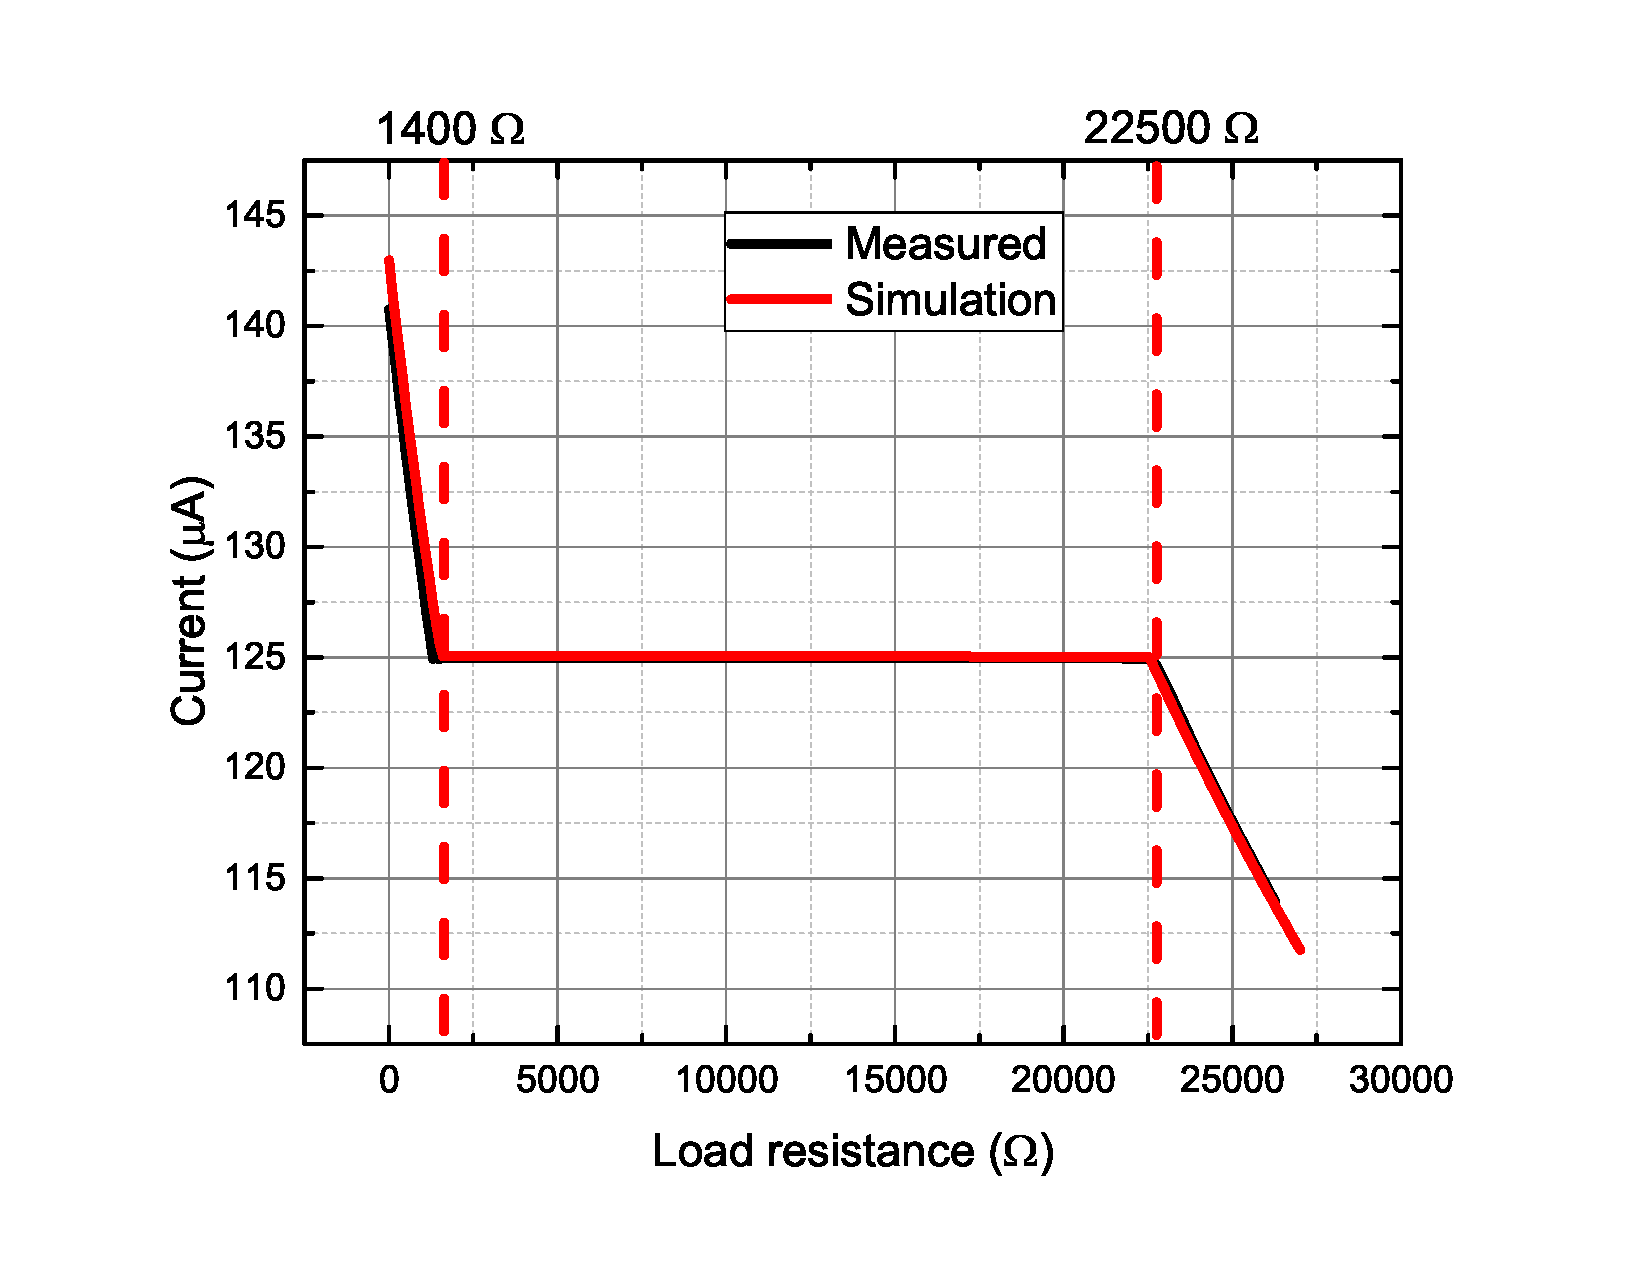
\includegraphics[width=0.9\paperwidth]{img/07/output_resistance.eps}
            \caption{Current sensor output characteristics}
            \label{Current_sensor_output_characteristics}
        \end{figure}

    \subsection{Temperature stability}
        Temperature was swept from $20$ to \SI{70}{\degreeCelsius}, no detectable changes were measured by the available meter, therefore it is assumed that current source fluctuates lower than about \SI{20}{\nano\ampere} in this temperature range.

\section{MOS settling}
    After enabling the measurement channel for the threshold voltage it takes a lot of time to fully stabilize its value. Instead of pre-enabling, same time method was used. ADC takes measurement of threshold voltage at precisely specified time after enabling power. In figure \ref{MOS_settling} 10 runs of measured voltage vs time are plotted, proving this method is stable within \SI{20}{\uV}.

    \begin{figure}[H]
        \centering
        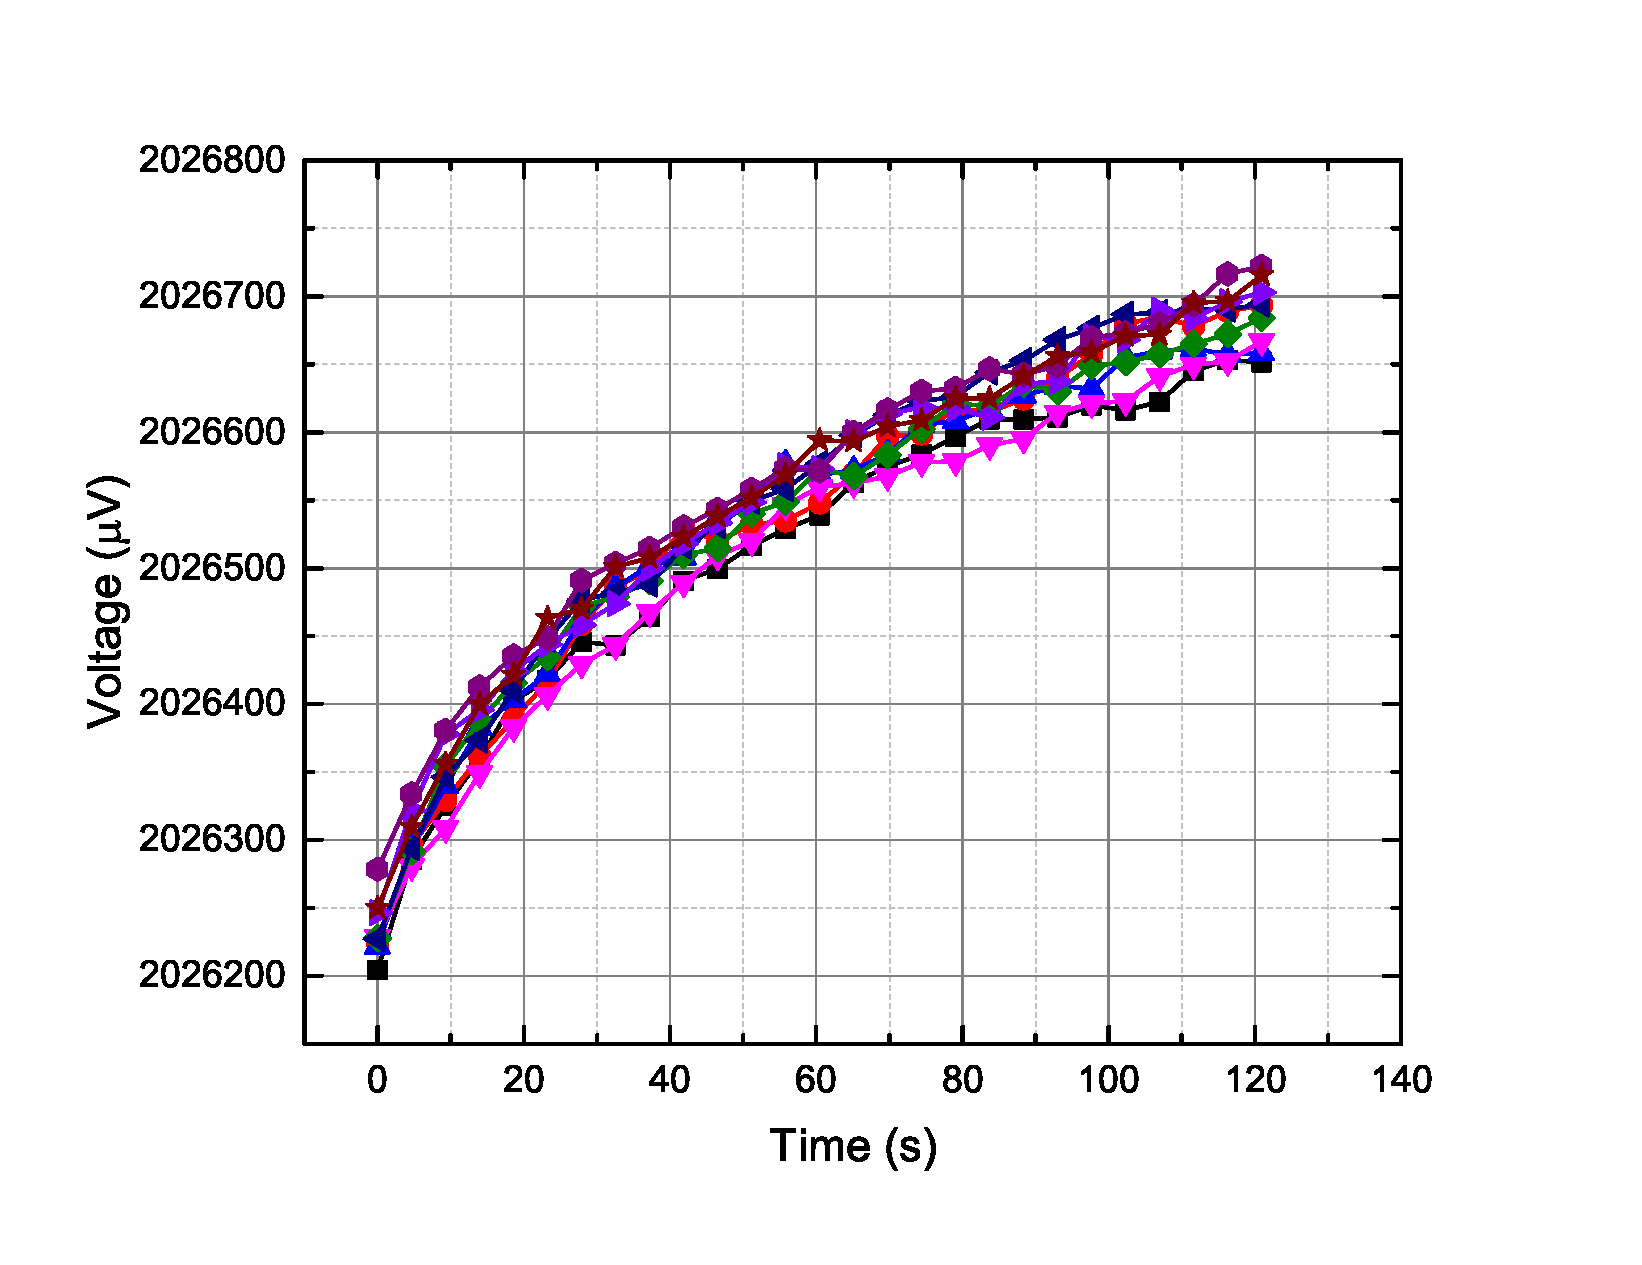
\includegraphics[width=0.8\paperwidth]{img/07/MOS_settling.eps}
        \caption{10 runs of MOS voltage setting}
        \label{MOS_settling}
    \end{figure}

\section{Measurement noise}
    The most important noise figure is system noise - ADC reading noise floor during nominal work.

    Because even the smallest temperature changes cause the ADC reading to shift (due to threshold/diode voltage shift) this efect had to be eliminated to measure noise. For this purpose a DC notch filter was used in post-processing, to eliminate any DC bias during measurement. The sampling frequency of the ADC was its nominal rate of \SI{0.25}{\hertz}. An example of filtration is shown in figure \ref{notch_DC_example}.

    \begin{figure}[H]
        \centering
        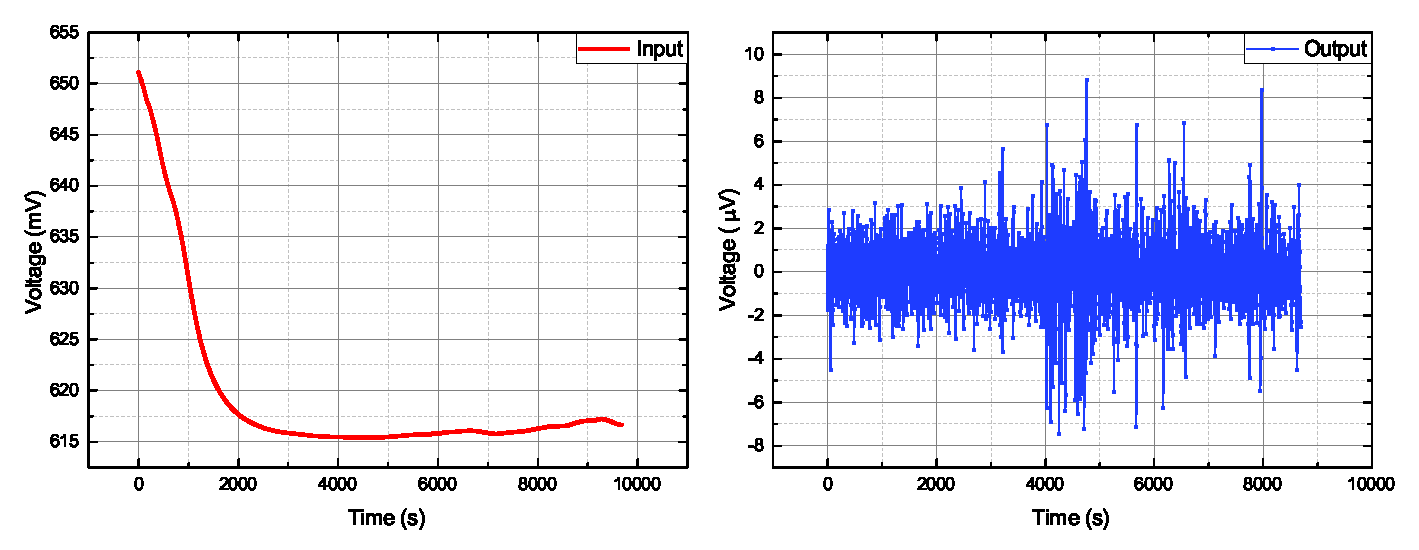
\includegraphics[width=0.8\paperwidth]{img/07/filterBeforeAfter.eps}
        \caption{Input and output of DC notch filter}
        \label{notch_DC_example}
    \end{figure}

    \subsection{Diode}
        \begin{figure}[H]
            \centering
            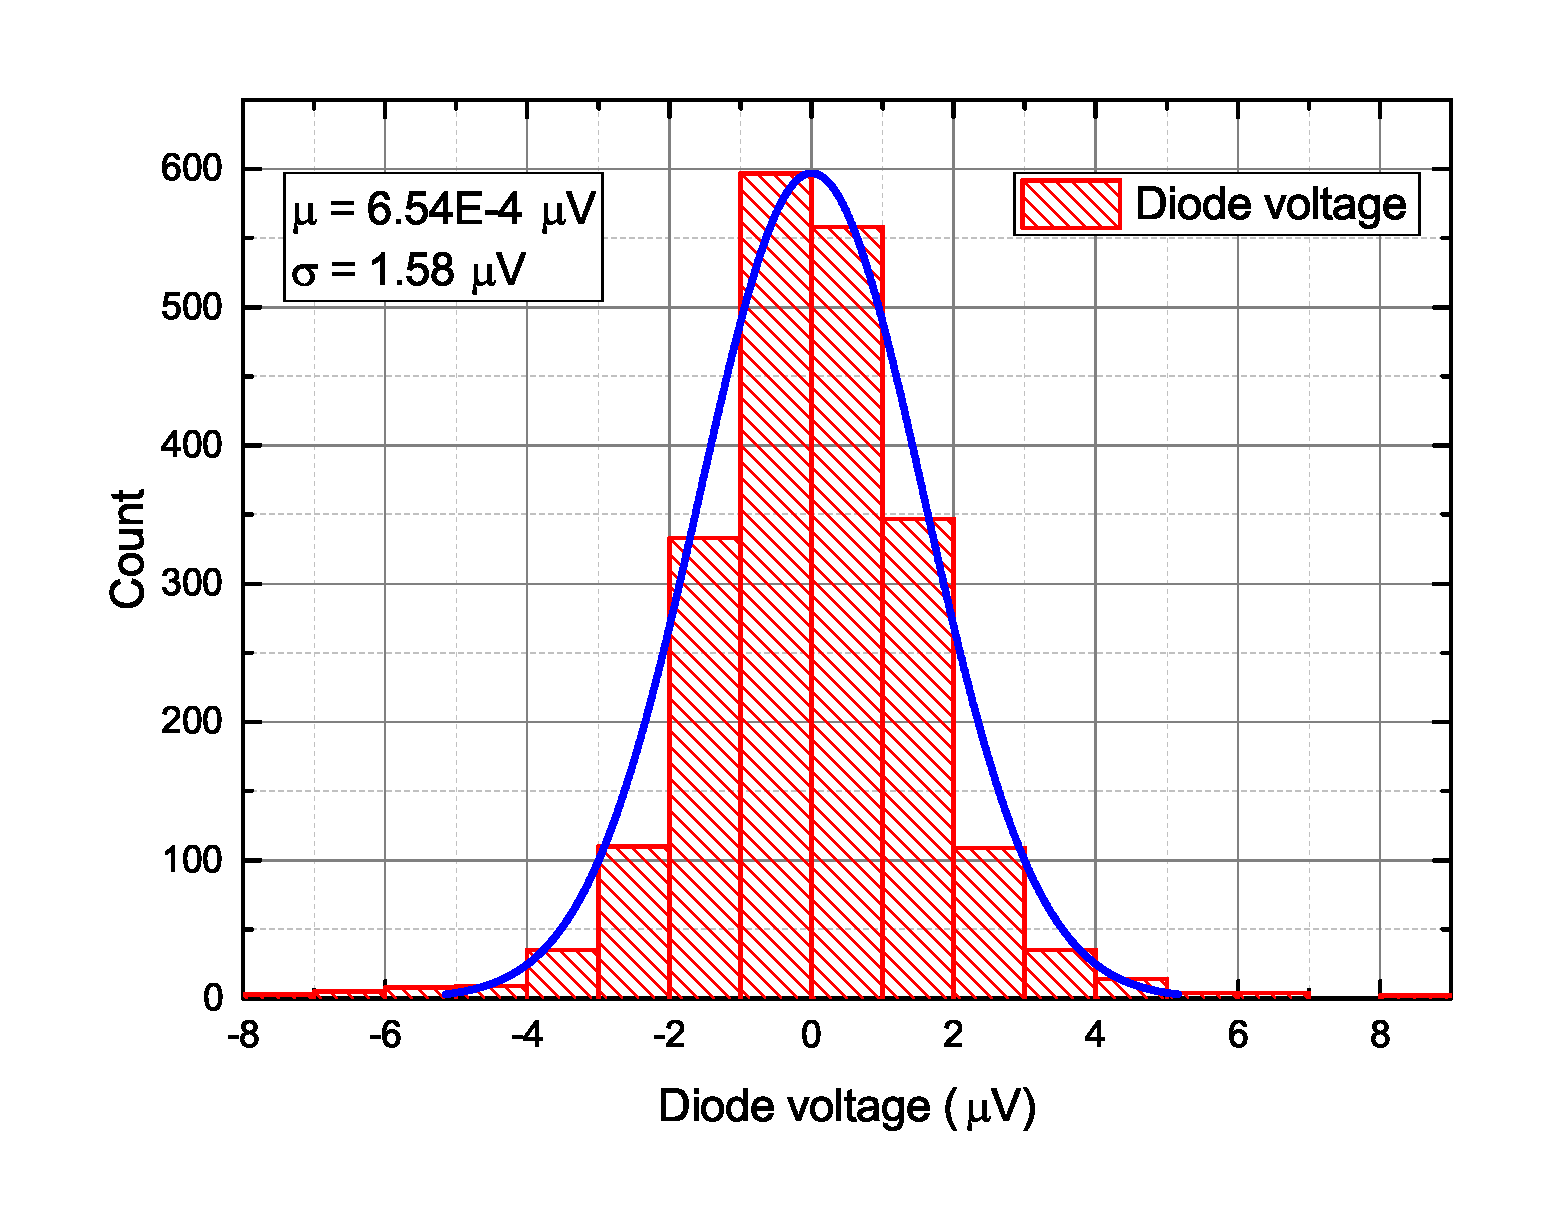
\includegraphics[width=0.6\paperwidth]{img/07/diodeVoltage.eps}
            \caption{Measured noise on body temperature channel}
        \end{figure}

        Noise on the temperature measurement channel has a standard deviation of $\SI{1.58}{\uV}$
    \subsection{Threshold voltage}
        \begin{figure}[H]
            \centering
            \includegraphics[width=0.6\paperwidth]{img/07/thresholdVoltageHistograms.eps}
            \caption{Measured noise on body temperature channel}
        \end{figure}

        Noise on the threshold voltage measurement channel has standard deviations of \SI{8.68}{\uV}, \SI{8.77}{\uV}, \SI{8.71}{\uV}.



    \subsection{Interpretation}
        Because the only difference between the temperature and threshold voltage channels is the semiconductor itself, the noise source can be estimated from the significant difference between them.

        The dependence between threshold voltage and drain current for this type of transistor was measured by M. Gumiela:
        $$I_D~[\mu A] = 410.376 \cdot (V_{TH} - 1.56457)^2 \text{~~~~~~Source: \ref{CD4007_p-MOSFET_transfer}}$$
        $$\frac{\textit{d}}{\textit{d}V_{TH}} I_D= 820.75 \cdot (-1.56 + V_{TH}) = \SI{439.46}{\uA/V} \text{~~~@ operating point}$$
        $$\textit{d}I_d = \SI{3.82}{\nA}$$
        Estimated equivalent current source have RMS value of $I_{N~RMS} = \SI{3.82}{\nA}$.

        This value is the same order of magnitude as calculated: reference voltage LT1634 has low-frequency noise of $U_N = \SI{15}{\uV}$ [TODO], this value is sensed directly across a series resistor, therefore $I_{NOISE} = U_N/R = \SI{1.5}{\nA}$. The left-hand side part of the noise equation can originate from different parts of the circuit, thermal and shot noise etc. % Noise output from LTSpice:



\section{Temperature characteristics}
    By placing the sensor in a thermal chamber and sweeping the temperature from \SI{0}{\degreeCelsius} up to \SI{75}{\degreeCelsius} temperature dependency charts were obtained for the device.

    \subsection{Diode}
        The diode response (figure \ref{Body_diode_temperature_dependency}) is almost ideally linear.
        \begin{figure}[H]
            \centering
            \includegraphics[width=0.6\paperwidth]{img/07/diodeVsTemperature.eps}
            \caption{Body diode temperature dependency}
            \label{Body_diode_temperature_dependency}
        \end{figure}


    \subsection{Threshold voltage}
        The threshold voltage (figure \ref{threshold_voltage_temperature_dependency}) tends to be non-linear, but it can be approximated as a quadratic function. Equation used: $V_{TH} = a \cdot t^2 + b \cdot t + c$, fitted parameters are shown in table \ref{vth_fit_params}.
        \begin{figure}[H]
            \centering
            \includegraphics[width=0.6\paperwidth]{img/07/thresholdVoltageTemperatureDependency.eps}
            \caption{Threshold voltage temperature dependency}
            \label{threshold_voltage_temperature_dependency}
        \end{figure}

        \begin{table}[H]
            \begin{center}
                \begin{tabular}{c|c|c|c}
                    Channel & a & b & c \\ \hline
                    ch 1 & $-0.00174~\pm~1.17011e-6$ & $-0.06692~\pm~8.33551e-5$ & $2027.53424~\pm~0.00125$ \\
                    ch 2 & $-0.00176~\pm~1.07318e-6$ & $-0.07437~\pm~7.64496e-5$ & $2028.72804~\pm~0.00114$ \\
                    ch 3 & $-0.00169~\pm~1.12071e-6$ & $-0.08736~\pm~7.98355e-5$ & $2036.83689~\pm~0.00119$ \\
                \end{tabular}
            \end{center}
            \caption{Temperature compensation results}
            \label{vth_fit_params}
        \end{table}

\section{Temperature compensation stability}
    The sensor should be compensated for temperature, with the assumption that temperature characteristic curves will not change during irradiation.

    During temperature sweep, data was gathered and post-processed, applying thermal compensation (given by charts \ref{Body_diode_temperature_dependency} and \ref{threshold_voltage_temperature_dependency}). In full sensing range, the sensor output shifts off the maximum $\SI{104}{\uV}$, which reflects TID measurement accuracy of about \SI{\pm 1}{\rad}. Note that TID dependency was not tested, but assumed according to \cite{COTSMosfetsGarcia}. Detailed accuracies are listed in table \ref{Temperature_compensation_results}.


    \begin{figure}[H]
        \centering
        \includegraphics[width=0.8\paperwidth]{img/07/compensatedThresholdVoltage.eps}
        \caption{Threshold voltage temperature compensation}
        \label{threshold_voltage_temperature_compensation}
    \end{figure}

    \begin{table}[H]
        \begin{center}
            \begin{tabular}{c|c|c|c}
                Channel & Standard deviation & Maximum difference & Accuracy ($3~\sigma$) \\ \hline
                ch 1 & \SI{15.13}{\uV} & \SI{89.40}{\uV} & \SI{\pm~0.0108}{\gray} = \SI{\pm~1.08}{\rad} \\
                ch 2 & \SI{16.27}{\uV} & \SI{103.24}{\uV} & \SI{\pm~0.0109}{\gray} = \SI{\pm~1.09}{\rad} \\
                ch 3 & \SI{15.36}{\uV} & \SI{101.26}{\uV} & \SI{\pm~0.0103}{\gray} = \SI{\pm~1.03}{\rad} \\
            \end{tabular}
        \end{center}
        \caption{Temperature compensation results}
        \label{Temperature_compensation_results}
    \end{table}

\chapter{Future work}

This chapter briefly describes the required steps for the sensor to be able to fly on-board PW-Sat2.

\section{Qualification model}
    Firstly, the sensor will be implemented on a PC-104 factor board, together with all final components and procedures. The model shown is taken from the design process (figure \ref{PLD_BOARD}).

    \begin{figure}[H]
        \centering
        \includegraphics[width=0.7\paperwidth]{img/08/PC104pldBoard.eps}
        \caption{PLD board with connector and space designed for RadFET}
        \label{PLD_BOARD}
    \end{figure}


    On this model all software tests (on flat-sat) will be carried out, as well as the final confirmation of design (thermal, radiation and time-stability tests). This board will qualify sensor design and software for flight use.

\section{Flight model}
    In the end, a final flight version of the PCB will be manufactured. In principle, it should be identical to the Qualification Model, but the handling procedures will be much more strict. Additionally, on the flight model, only thermal calibration will be made, without further stress-testing. During integration, the final version of the sensor on PC104-board will be placed on the electronics stack inside PW-Sat2.

\chapter{Summary}
    Engineering model of the sensor was designed and preliminary tested. This is solid foundation to further work, which will result in flight-ready version of the sensor. This model allowed to test concept and possible solutions of sensor components, proving the design.

    Tests have proven fidelity of measurements - assumed resolution and range are beyond required. Designed sensor parameters are shown in table \ref{sensor_results_parameters}.

    \begin{table}[H]
        \begin{center}
            \begin{tabular}{r|l}
                \textbf{Parameter} & \textbf{Result} \\ \hline
                Sensor resolution & \SI{0.003}{\rad}, \\
                Sensor accuracy & \SI{1}{\rad}, \\
                Sensor range & \SI{10}{\kilo\rad}, \\
                Operating temperature range & \SI{0}{\degreeCelsius} to \SI{70}{\degreeCelsius}, \\
                Communication protocol & $I^2C$, \\
                Sensor supply voltage & \SI{5}{\volt}, \\
                Sensor power consumption & \SI{0.125}{\watt}, \\
                Radiation tolerance & $>~\SI{15}{\kilo\rad}$ \\

            \end{tabular}
        \end{center}
        \caption{Finished sensor parameters}
        \label{sensor_results_parameters}
    \end{table}

    Thesis resulted in fully integrated, ready to use sensor which can be used as a preliminary calibration check model. It was designed having in mind space environment, limitations and requirements of CubeSat satellite. During testing, sensor proved its design by conducted tests. Moreover, its size and requirements on the bus are limited, broaden possibilities of manufacturing this sensor as a separate module, for other CubeSat missions.

    As a next steps, this model have to be tested more throughly - especially radiation tests and calibration. Later, qualification and flight models would be manufactured, hopefully leading to sensor launch on PW-Sat2 satellite at the end of year 2017, where it can be tested in target space conditions.




\appendix
\printbibliography

\end{document}
